	
\RequirePackage[l2tabu, orthodox]{nag}
\documentclass[
	twoside, 
	openany, 
	11pt,
	bibliography=totoc,
]{scrreprt}

\usepackage{rerunfilecheck}

%%	(c) 2014-2018 Benjamin Steinwender KAI GmbH
%% 
%%	This file provides the style and recommended packages for 
%%	a KAI software documentation LaTeX project.
%%

%	prepare a symbols-list (package glossaries)
\newif\ifusesymbols

%	don't print single occurences:	http://tex.stackexchange.com/questions/98494
\newif\ifnosingle


%\usepackage[
%	chapter,
%	cache=false,
%]{minted}
%\setminted{
%	autogobble=true,
%	linenos,
%	tabsize=4,
%	fontsize=\small,
%}

\usepackage[utf8]{inputenc}
\usepackage[T1]{fontenc}
\usepackage[LGRgreek]{mathastext}
\usepackage[
	usenames,
	dvipsnames,
	svgnames,
	table,
]{xcolor}
\usepackage[
	prefix=sol-,
]{xcolor-solarized}


\usepackage{array}
\usepackage{tabularx}
\usepackage{tikz}
\usetikzlibrary{positioning,shapes,shadows,arrows}
\usepackage{graphicx}
\usepackage{fancyhdr}
\usepackage{subcaption}
\usepackage{caption}
\usepackage{float}
\usepackage{longtable}
\usepackage{listings}
\lstset{language=C,
	basicstyle=\small,
	keywordstyle=\color{black}\bfseries\underbar,
	identifierstyle=,
	commentstyle=\color{white},
	stringstyle=\ttfamily,
	showstringspaces=false}

\graphicspath{ {./images/} }


%\usepackage[
%	chapter,
%	cache=false,
%]{minted}
%\setminted{
%	autogobble=true,
%	linenos,
%	tabsize=4,
%	fontsize=\small,
%}

\floatstyle{plaintop}\restylefloat{listing}	%	set the listing-caption above

\usepackage{scrhack}	%	fixes add float to lists - must be loaded after minted

\usepackage[ngerman,english]{babel}
\usepackage{csquotes}
\usepackage[	%	http://tex.stackexchange.com/questions/5091
	backend=bibtex,
	backref=true,
	sorting=none,	%	sorting of citations: none = in order
	style=ieee,
	dashed=false,
]{biblatex}

% https://tex.stackexchange.com/questions/451192
\usepackage{silence}
\WarningFilter{biblatex}{File 'english-ieee.lbx'}
\WarningFilter{biblatex}{File 'german-ieee.lbx'}
\WarningFilter{biblatex}{File 'ngerman-ieee.lbx'}

\usepackage{xfrac}
% C code
\definecolor{mGreen}{rgb}{0,0.6,0}
\definecolor{mGray}{rgb}{0.5,0.5,0.5}
\definecolor{mPurple}{rgb}{0.58,0,0.82}
\definecolor{backgroundColour}{rgb}{0.95,0.95,0.92}

\usepackage[
	version-1-compatibility,
	alsoload=binary,
	binary-units,
	per=slash,
]{siunitx}

\sisetup{
	inter-unit-product = $\cdot$,
	list-final-separator = { \translate{and} },
	list-pair-separator = { \translate{and} },
	range-phrase = { \translate{to (numerical range)} },
	scientific-notation = engineering,	%	exponent is always a power of 3
	exponent-to-prefix,
	exponent-product = \cdot,
	round-precision = 2,
	round-mode = places,
	detect-weight=true,
	detect-family=true,
}

%	textcomp provides the textmu version that microtype can handle with siunitx
%		see http://tex.stackexchange.com/questions/74670
\usepackage{textcomp}
\usepackage{microtype}


%Plots
\usepackage{pgfplots}
\pgfplotsset{compat=1.5}

%Redefine the underscore command
\let\underscore\_
\newcommand{\myunderscore}{\renewcommand{\_}{\underscore\hspace{0pt}}}

%font alignment
\renewcommand{\baselinestretch}{1.00} 

\usepackage[
	unicode=true,			%	non-Latin characters in Acrobat�s bookmarks
	hypertexnames=true,		%	fixes ``destination with the same identifier'' warning
	bookmarks=true,			%	show bookmarks bar?
	bookmarksnumbered=true,
	bookmarksopen=false,
%	breaklinks=true,		%	set true to word wrap long lines in listof* properly
	pdfborder={0 0 0},
%	pagebackref=true,		%	true|false	%	included in biblatex
	colorlinks=true,		%	true: colored links; false: boxes around the link
%	ocgcolorlinks=true,		%	Optional Content Groups - colored links, when viewed, but printed without colors: http://tex.stackexchange.com/questions/230752
	linkcolor=sol-blue,		%	color of internal links (change box color with linkbordercolor)
	citecolor=sol-green,	%	color of links to bibliography
	filecolor=sol-magenta,	%	color of file links
	urlcolor=sol-cyan,		%	color of external links
%	pdfauthor={Yashas Udupa},	%	author
]{hyperref}
\hypersetup{
%	pdftoolbar=true,		% show Acrobat�s toolbar?
%	pdfmenubar=true,		% show Acrobat�s menu?
	pdffitwindow=true,		% window fit to page when opened
	pdfstartview={FitH},	% fits the width of the page to the window
%	pdfsubject={Subject},	% subject of the document
%	pdfcreator={Creator},	% creator of the document
%	pdfproducer={Producer},	% producer of the document
%	pdfkeywords={keyword1, key2, key3}, % list of keywords
	pdfnewwindow=true,		% links in new PDF window
}

%List of acronyms
%\usepackage[nopostdot,nogroupskip,style=super,nonumberlist,toc,automake,toc]{glossaries} %Load glossaries package
%	glossaries must be loaded after hyperref
\usepackage{mfirstuc}
\usepackage{mfirstuc-english}
\usepackage{makeidx}
\usepackage[
	toc,			%	include in table of contents
	nonumberlist,	%	suppress the location list
	%nogroupskip,	%	suppress alphabetic grouping of entries
	nomain,
%	nopostdot,		%	suppress terminating dot
	acronym,		%	add acronyms
	notree,			%	no tree formats
	shortcuts,		%	shortcut commands (ac, acs, acl, acp, ...)
	savewrites,		%	reduce number of \write streams
]{glossaries}
%\usepackage[xindy,
 %           toc,
  %          section,
   %         acronym]{glossaries}
\ifusesymbols
\newglossary[slg]{symbolslist}{syi}{syg}{Symbols}
\fi

%	non-breakable space between long and short form
\renewcommand*{\glsacspace}[1]{~}

%	use the description on first use,
\newacronymstyle{descfirst-long-sp-short}{%
	\GlsUseAcrEntryDispStyle{long-short}%
}{%
	\GlsUseAcrStyleDefs{long-short}%
	\renewcommand*{\genacrfullformat}[2]{%
		\glsentrydesc{##1}##2\glsacspace{##1}%
		(\protect\firstacronymfont{\glsentryshort{##1}})%
	}%
	\renewcommand*{\Genacrfullformat}[2]{%
		\Glsentrydesc{##1}##2\glsacspace{##1}%
		(\protect\firstacronymfont{\glsentryshort{##1}})%
	}%
	\renewcommand*{\genplacrfullformat}[2]{%
		\glsentrydescplural{##1}##2\glsacspace{##1}%
		(\protect\firstacronymfont{\glsentryshortpl{##1}})%
	}%
	\renewcommand*{\Genplacrfullformat}[2]{%
		\Glsentrydescplural{##1}##2\glsacspace{##1}%
		(\protect\firstacronymfont{\glsentryshortpl{##1}})%
	}%
}

\setacronymstyle{%
	descfirst-long-sp-short%custom format: see directly above
%	long-short%	on first use display the long form with the short form in parentheses
%	short-long%	on first use display the short form with the long form in parentheses
%	long-short-desc%	like long-short but you need to specify the description
%	short-long-desc%	like short-long but  you  need  to  specify  the  description
%	footnote%	on first use display the short form with a footnote on the page
%	dua%	always expand
}

%	cleveref must be loaded after hyperref
\usepackage[
	capitalize,
	nameinlink,
	noabbrev,
]{cleveref}

%	header style
%\usepackage[
%	automark,
%	headsepline,
%]{scrlayer-scrpage}
%\clearpairofpagestyles
%\cfoot[\pagemark]{\pagemark}
%\lehead{\headmark}
%\rohead{\headmark}
%\pagestyle{scrheadings}

%	paragraph settings
\setlength{\parskip}{3ex plus 2ex minus 2ex}
\linespread{1.1}

\renewcommand{\floatpagefraction}{0.9}
\renewcommand{\textfraction}{0.05}
\renewcommand{\topfraction}{1.0}
\renewcommand{\bottomfraction}{1.0}

\usepackage[all]{nowidow}

%\usepackage[acronym,nomain,nonumberlist]{glossaries}

%	don't print single occurences:	http://tex.stackexchange.com/questions/98494
\ifnosingle
\glsenableentrycount	%	enable \cgls, \cglspl, \cGls, \cGlspl
\let\gls\cgls
\let\glspl\cglspl
\let\Gls\cGls
\let\Glspl\cGlspl
\fi

%	load as very last package!
\usepackage[shortcuts]{extdash}

% prepare the acronyms and symbols list
%	you can provide your own version of \glsmark
%	if not, it will be declared here
\ifdef{\glsmark}{}{%
%	\newcommand*{\glsmark}[1]{#1}% no modification
%	\newcommand*{\glsmark}[1]{\underline{#1}}%
	\newcommand*{\glsmark}[1]{\uppercase{#1}}%
}

%	abbreviations here:
%		the description will be used on the first expansion and on the acronym list
%		the long text will be used when only one instance is used (i.e. plain english text)
\newacronym{2DEG}		{2DEG}		{two-dimensional electron gas}

\newacronym[
	description={\glsmark{a}lternating \glsmark{c}urrent},
]{AC}			{AC}		{alternating current}
\newacronym[
	description={\glsmark{A}ctive \glsmark{C}ycle \glsmark{U}niversal \glsmark{T}est \glsmark{E}quipment},
]{ACUTE}		{ACUTE}		{Active Cycle Universal Test Equipment}
\newacronym{AD}			{A/D}		{Analog-to-Digital}
%\newacronym{ADC}		{ADC}		{Analog-to-Digital Conversion}	%	conflict, please copy or create your own
%\newacronym{ADC}		{ADC}		{Analog-to-Digital Converter}	%	conflict, please copy or create your own
%\newacronym[
%	description={\glsmark{A}utomotive \glsmark{E}lectronics \glsmark{C}ouncil},
%]{AEC}		{AEC}		{Automotive Electronics Council} % replaced by glossary entry
\newacronym{AlGaN}		{AlGaN}		{Aluminium Gallium Nitride}
\newacronym[
	description={\glsmark{a}rithmetic \glsmark{l}ogic \glsmark{u}nit}
]{ALU}		{ALU}		{arithmetic logic unit}
\newacronym[
	description={\glsmark{a}nisotropic \glsmark{m}agneto \glsmark{r}esistance}
]{AMR}		{AMR}		{anisotropic magneto resistance}
\newacronym[
	description={\glsmark{A}pplication \glsmark{P}rogramming \glsmark{I}nterface},
]{API}		{API}		{application programming interface}
\newacronym[
	description={\glsmark{A}dvanced \glsmark{R}epetitive \glsmark{C}lamping \glsmark{T}est \glsmark{I}ntegrated \glsmark{S}ystem},
]{ARCTIS}		{ARCTIS}	{Advanced Repetitive Clamping Test Integrated System}
%\newacronym{ARM}		{ARM}		{Advanced {\glsentryshort{RISC}} Machines}	%	conflict, please copy or create your own
\newacronym{ASIC}		{ASIC}		{Application-specific Integrated Circuit}
\newacronym{ATE}		{ATE}		{Automated Test Equipment}
\newacronym{ATML}		{ATML}		{Automatic Test Markup Language}
\newacronym{AToM}		{AToM}		{Automatic Testing of MoPS}
\newacronym{AUX}		{AUX}		{Auxiliary}

\newacronym{BGA}		{BGA}		{Ball Grid Array}
\newacronym{BIST}		{BIST}		{Built-In Self-Test}
\newacronym[
	description={\glsmark{b}ipolar \glsmark{j}unction \glsmark{t}ransistor}
]{BJT}		{BJT}		{bipolar junction transistor}
\newacronym{BMP}		{BMP}		{bitmap}

\newacronym{CAN}		{CAN}		{Controller Area Network}
\newacronym{CCAN}		{CCAN}		{Comprehensive C Archive Network}
\newacronym[
	description={\glsmark{c}umulative \glsmark{d}ensity \glsmark{f}unction}
]{CDF}		{CDF}		{cumulative density function}
\newacronym{CDIR}		{CDIR}		{Classless Inter-Domain Routing}
\newacronym{CiA}		{CiA}		{{\acrshort{CAN}}-in-Automation}
\newacronym{CoE}		{CoE}		{CANopen over EtherCAT}
\newacronym{CGPM}		{CGPM}		{Conférence Générale des Poids et Mesures (General Conference on Weights and Measures)}
\newacronym{CM}			{CM}		{Common Mode}
\newacronym[
	description={\glsmark{c}omplementary \glsmark{m}etal–\glsmark{o}xide–\glsmark{s}emiconductor},
]{CMOS}		{CMOS}		{complementary metal–oxide–semiconductor}
\newacronym{CMRR}		{CMRR}		{Common Mode Rejection Ratio}
\newacronym{CMTI}		{CMTI}		{Common Mode Transient Immunity}
\newacronym{CORBA}		{CORBA}		{Common Object Request Broker Architecture}
\newacronym{COTS}		{COTS}		{Commercial off-the-shelf}
\newacronym{CPHA}		{CPHA}		{Clock Phase}
\newacronym{CPOL}		{CPOL}		{Clock Polarity}
\newacronym{CPU}		{CPU}		{Central Processing Unit}
\newacronym{CQR}		{CQR}		{Communication Quality Rating}
\newacronym{CRC}		{CRC}		{Cyclic Redundancy Check}
\newacronym{CS}			{CS}		{Carrier Sense}
\newacronym{CSS}		{CSS}		{Cascading Style Sheet}
\newacronym{CSMA}		{CSMA}		{Carrier Sense Multiple Access}
\newacronym{CSMA/CA}	{CSMA/CA}	{Carrier Sense Multiple Access / Collision Avoidance}
\newacronym{CSMA/CD}	{CSMA/CD}	{Carrier Sense Multiple Access / Collision Detection}
\newacronym{CSMA/CR}	{CSMA/CR}	{Carrier Sense Multiple Access / Collision Resolution}
\newacronym[
	description={\glsmark{c}urrent \glsmark{t}ransformer}
]{CT}			{CT}		{current transformer}
\newacronym{CTE}		{CTE}		{Coefficient of Thermal Expansion}
\newacronym{CUAS}		{CUAS}		{Carinthia University of Applied Sciences}

\newacronym[
	longplural={Devices Under Test},
	shortplural={DUTs},
	description={\glsmark{d}evice \glsmark{u}nder \glsmark{t}est},
]			{DUT}		{DUT}		{device under test}
\newacronym{DA}			{D/A}		{Digital-to-Analog}
%\newacronym{DAC}		{DAC}		{Digital-to-Analog Conversion}	%	conflict, please copy or create your own
%\newacronym{DAC}		{DAC}		{Digital-to-Analog Converter}	%	conflict, please copy or create your own
\newacronym{DAP}		{DAP}		{Device Access Port}
\newacronym{DAQ}		{DAQ}		{Data AcQuisition}
\newacronym{DAVE}		{DAVE}		{Digital Application Virtual Engineer}
\newacronym{DC}			{DC}		{Direct Current}
\newacronym{DHCP}		{DHCP}		{Dynamic Host Configuration Protocol}
\newacronym{DGD}		{DGD}		{Diagnostic Gate Driver}
\newacronym{DIO}		{DIO}		{Digital Input Output}
\newacronym{DIP}		{DIP}		{Dual In-line Package}
\newacronym{DL}			{DL}		{Data Logger}
\newacronym{DLL}		{DLL}		{Dynamic Link Library}
\newacronym{DLMS}		{DLMS}		{Device Level Maverick Screening}
\newacronym{DMA}		{DMA}		{Direct Memory Access}
\newacronym{DMOS}		{DMOS}		{Double diffused {\acrshort{MOS}} transistor}
\newacronym{DOE}		{DOE}		{Design of Experiments}
\newacronym{DoE}		{DoE}		{Design of Experiment}
\newacronym{DoS}		{DoS}		{Denial-of-Service}
\newacronym{DRAM}		{DRAM}		{Dynamic {\glsentryshort{RAM}}}
\newacronym{DSD}		{DSD}		{Delta-Sigma Demodulator}
\newacronym{DSP}		{DSP}		{Digital Signal Processor}
\newacronym{DTD}		{DTD}		{Document Type Declaration}
\newacronym{DTLS}		{DTLS}		{Datagram Transport Layer Security}

\newacronym{EAGLE}		{EAGLE}		{Easily Applicable Graphical Layout Editor}
\newacronym{EAM}		{EAM}		{Institut für Elektrische Antriebstechnik und Maschinen an der TU Graz}
\newacronym{ECU}		{ECU}		{Embedded Control Unit}
\newacronym{EBU}		{EBU}		{External Bus Unit}
\newacronym{EDF}		{EDF}		{Earliest Deadline First}
\newacronym[
	description={\glsmark{e}lectronic \glsmark{d}ata \glsmark{s}heet},
]{EDS}		{EDS}		{electronic data sheet}

\newacronym[
	description={\glsmark{}lectromagnetic \glsmark{c}compatibility},
]{EMC}		{EMC}		{electromagnetic compatibility}
\newacronym{EMI}		{EMI}		{Electromagnetic Interference}
\newacronym{EoE}		{EoE}		{Ethernet over EtherCAT}
\newacronym{EOL}		{EOL}		{End of Life}
\newacronym{EEPROM}		{EEPROM}	{Electrically Erasable Programmable Read-Only Memory }
\newacronym{ERU}		{ERU}		{Event Request Unit}
\newacronym[
	description={\glsmark{e}lastic \glsmark{s}lot \glsmark{b}oundary}
]{ESB}		{ESB}		{elastic slot boundary}
\newacronym{ESD}		{ESD}		{Electro-Static Discharge}
\newacronym[
	description={\glsmark{e}quivalent \glsmark{s}eries \glsmark{i}nductance}
]{ESL}		{ESL}		{equivalent series inductance}
\newacronym{ET}			{ET}		{Event Triggered}
\newacronym{EtherCAT}	{EtherCAT}	{Ethernet for Control Automation Technology}

\newacronym{FCE}		{FCE}		{Flexible CRC Engine}
\newacronym{FCFS}		{FCFS}		{First Come First Serve}
\newacronym{FDD}		{FDD}		{Fault Detection and Diagnosis}
\newacronym{FDI}		{FDI}		{Fault Detection and Isolation}
\newacronym{FET}		{FET}		{Field Effect Transistor}
\newacronym{FEM}		{FEM}		{Finite Element Method}
\newacronym{FIFO}		{FIFO}		{First In First Out}
\newacronym[
	description={\glsmark{f}ield \glsmark{p}rogrammable \glsmark{g}ate \glsmark{a}rray},
]{FPGA}		{FPGA}		{field programmable gate array}
\newacronym{FMMU}		{FMMU}		{Fieldbus Memory Management Unit}
\newacronym{FMS}		{FMS}		{Fieldbus Message Specification}
\newacronym{FoE}		{FoE}		{File access over EtherCAT}
\newacronym{FTT}		{FTT}		{Flexible Time Triggered}
\newacronym[
	description={\glsmark{f}inite-\glsmark{s}tate \glsmark{m}achine},
]{FSM}		{FSM}		{finite-state machine}
\newacronym{FTP}		{FTP}		{File Transfer Protocol}
\newacronym{GaN}		{GaN}		{Gallium Nitride}
\newacronym[
	description={\glsmark{g}iant \glsmark{m}agneto \glsmark{r}esistance}
]{GMR}		{GMR}		{giant magneto resistance}
\newacronym{GPIB}		{GPIB}		{General Purpose Interface Bus}
\newacronym{GPIO}		{GPIO}		{General Purpose Input Output}
\newacronym[
	description={\glsmark{g}raphical \glsmark{u}ser \glsmark{i}nterface},
]{GUI}		{GUI}		{graphical user interface}
\newacronym{HEMT}		{HEMT}	{High Electron Mobility Transistor}
\newacronym{HDL}		{HDL}		{Hardware Description Language}
\newacronym{HID}		{HID}		{Human Interface Device}
\newacronym[
	description={\glsmark{h}ardware-\glsmark{i}n-the-\glsmark{l}oop},
]{HIL}		{HIL}		{hardware-in-the-loop}
\newacronym{HRO}		{HRO}		{High Resolution Oscilloscope}
\newacronym{HTFB}		{HTFB}		{High Temperature Forward Bias}
\newacronym{HTGB}		{HTGB}		{High Temperature Gate Bias}
\newacronym{HTML}		{HTML}		{Hyper Text Markup Language}
\newacronym{HTRB}		{HTRB}		{High Temperature Reverse Bias}
\newacronym[
	description={\glsmark{h}igh \glsmark{t}emperature \glsmark{o}perating \glsmark{l}ife},
]{HTOL}		{HTOL}		{High Temperature Operating Life}
\newacronym{HTSL}		{HTSL}		{High Temperature Storage Live Test}
\newacronym{HV}			{HV}		{High Voltage}
\newacronym{HW}			{HW}		{hardware}

\newacronym{IC}			{IC}		{Integrated Circuit}
\newacronym{ID}			{ID}		{Identification}
\newacronym[
	description={\glsmark{i}ntegrated \glsmark{d}evelopment \glsmark{e}nvironment}
]{IDE}		{IDE}		{integrated development environment}
\newacronym{Idrv}		{Idrv}		{Driver current}
\newacronym{IEC}		{IEC}		{International Electrotechnical Commission}
\newacronym{IFAT}		{IFAT}		{Infineon Technologies Austria AG}
\newacronym{IFS}		{IFS}		{Interface File System}
\newacronym{IGBT}		{IGBT}		{Insulated Gate Bipolar Transistor}
\newacronym{IIC}		{IIC}		{Inter-Integrated Circuit}
\newacronym{Iin}		{Iin}		{Converter input current}
\newacronym{I2C}		{I\textsuperscript{2}C}	{Inter-Integrated Circuit}
\newacronym{Imon}			{Imon}		{IC current monitor}
\newacronym{IO}			{IO}		{Input \& Output}
\newacronym{IoT}		{IoT}		{Internet of Things}
\newacronym{Iout}		{Iout}		{Converter output current}
%	conflict, please copy or create your own
%\newacronym{IP}			{IP}		{Intellectual Property}
%\newacronym{IP}			{IP}		{Internet Protocol}
\newacronym[
	description={\glsmark{I}nternet \glsmark{p}rotocol},
]{IPv4}		{IP}		{Internet protocol}
\newacronym{ISO}		{ISO}		{International Organization for Standardization}
\newacronym{ISR}		{ISR}		{Interrupt Service Routine}
\newacronym{ITS-90}		{ITS-90}	{International Temperature Scale of 1990}

%\newacronym{JEDEC}		{JEDEC}		{Joint Electron Device Engineering Council}	% moved to glossary
\newacronym[
	description={\glsmark{J}ava\glsmark{S}cript \glsmark{o}bject \glsmark{n}otation},
]{JSON}					{JSON}		{JavaScript object notation}
\newacronym{JTAG}		{JTAG}		{Joint Test Action Group}

\newacronym[
	description={\glsmark{K}ompetenzzentrum \glsmark{A}utomobil- und \glsmark{I}ndustrie-Elektronik},
]{KAI}		{KAI}		{Kompetenzzentrum Automobil- und Industrie-Elektronik}
\newacronym{KATE}		{KA$^2$TE}	{{\acrshort{KAI}} {\acrshort{ACUTE}} \& {\acrshort{ARCTIS}} Test Environment}

\newacronym{LabVIEW}	{LabVIEW}	{Laboratory Virtual Instrument Engineering Workbench}
\newacronym[
	description={\glsmark{l}ocal \glsmark{a}rea \glsmark{n}etwork},
]{LAN}		{LAN}		{local area network}
\newacronym[
	description={\glsmark{l}ow \glsmark{d}ropout \glsmark{l}linear \glsmark{r}egulator},
]{LDO}		{LDO}		{low dropout linear regulator}
\newacronym{LED}		{LED}		{Light Emitting Diode}
\newacronym[
	description={\glsmark{l}inear \glsmark{f}eet \glsmark{p}er \glsmark{m}inute},
]{LFM}		{LFM}		{linear feet per minute}
\newacronym{LQR}		{LQR}		{Linear Quadratic Regulator}
\newacronym{LSB}		{LSB}		{Least Significant Bit}
\newacronym{LTOL}		{LTOL}		{Low Temperature Operating Life}
\newacronym{LUFA}		{LUFA}		{Lightweight USB Framework for AVRs}
\newacronym{LUT}		{LUT}			{LookUp-Table}
\newacronym{LV}			{LV}		{Low Voltage}
\newacronym{LXI}		{LXI}		{{\glsentryshort{LAN}} eXtensions for Instrumentation}

\newacronym{MA}			{MA}		{Multiply-Accumulate}
\newacronym{MAC}		{MAC}		{Medium Access Control}
\newacronym{MAX}		{MAX}		{Measurement \& Automation eXplorer}
\newacronym{MCU}		{MCU}		{Micro Controller Unit}
\newacronym{MEDL}		{MEDL}		{\glsmark{Me}ssage \glsmark{D}escriptor \glsmark{L}ist}
\newacronym{MISO}		{MISO}		{Master Input - Slave Output}
\newacronym[
	description={\glsmark{m}ulti\glsmark{l}ayer \glsmark{c}eramic \glsmark{c}apacitors},
]{MLCC}		{MLCC}		{multilayer ceramic capacitors}
\newacronym{MO}			{MO}		{Message Object}
\newacronym[
	description={\glsmark{m}odular \glsmark{p}ower \glsmark{s}tress},
]{MoPS}		{MoPS}		{modular power stress}
\newacronym{MOS}		{MOS}		{Metal Oxide Semiconductor}
\newacronym{MOSFET}		{MOSFET}	{Metal-Oxide Semiconductor Field Effect Transistor}
\newacronym{MMU}		{MMU}		{Memory Management Unit}
\newacronym{MOSI}		{MOSI}		{Master Output - Slave Input}
\newacronym[
	description={\glsmark{m}agneto \glsmark{r}esistance}
]{MR}			{MR}		{magneto resistance}
\newacronym[
	description={\glsmark{m}odular \glsmark{t}est \glsmark{s}ystem},
]{MTS}			{MTS}		{modular test system}
\newacronym{MSB}		{MSB}		{Most Significant Bit}
\newacronym{MTTF}		{MTTF}		{Mean Time To Failure}
\newacronym{MUX}		{MUX}		{Multiplexer}
\newacronym{MVC}		{MVC}		{Model–View–Controller}
\newacronym{MV}			{MV}		{Mid Voltage}
%\newacronym{NDA}		{NDA}		{Non Destructive Arbitration}	%	conflict, please copy or create your own
\newacronym{NI}			{NI}		{National Instruments}
\newacronym{NIC}		{NIC}		{Network Interface Card}
\newacronym{NRZI}		{NRZI}		{Non-Return-to-Zero-Inverted}
\newacronym{NTC}		{NTC}		{Negative Temperature Coefficient}

\newacronym{OC}			{OC}		{Over-Current}
\newacronym{OL}			{OL}		{Open-Load}
\newacronym[
	description={\glsmark{o}perational \glsmark{a}mplifier},
]{OpAmp}		{OpAmp}		{operational amplifier}
\newacronym{OS}			{OS}		{\glsmark{o}perating \glsmark{s}ystem}
\newacronym{OSI}		{OSI}		{Open Systems Interconnect}
\newacronym{OT}			{OT}		{Over-Temperature}

\newacronym{PAT}		{PAT}		{Part Average Testing}
\newacronym{PC}			{PC}		{Personal Computer}
\newacronym[
	description={\glsmark{p}rinted \glsmark{c}ircuit \glsmark{b}oard},
]{PCB}		{PCB}		{printed circuit board}
\newacronym{PCI}		{PCI}		{Peripheral Component Interconnect}
%\newacronym{PDF}		{PDF}		{\glsmark{P}ortable \glsmark{D}ocument \glsmark{F}ormat}	%	conflict, please copy or create your own
%\newacronym{PDF}		{PDF}		{\glsmark{P}robability \glsmark{D}ensity \glsmark{F}unction}	%	conflict, please copy or create your own
\newacronym{PDO}		{PDO}		{Process Data Object}
\newacronym{PDU}		{PDU}		{Protocol Data Unit}
\newacronym{PEM}		{PEM}		{Photo Emission Microscopy}
\newacronym{PFC}		{PFC}		{Power Factor Correction}
\newacronym{PHY}		{PHY}		{Physical Layer}
\newacronym{PI}		{PI}		{Proportional-Integral}
%	conflict, please copy or create your own
%\newacronym{PID}		{PID}		{Proportional-Integral-Derivative}
%\newacronym{PID}		{PID}		{Product ID}
\newacronym{PLC}		{PLC}		{Programmable Logic Controller}
\newacronym{PNG}		{PNG}		{Portable Network Graphics}
\newacronym{PoL}		{PoL}		{Point-of-Load}
\newacronym{PROFIBUS}	{PROFIBUS}	{PROcess FIeld BUS}
\newacronym{PDP}		{PROFIBUS DP}	{{\glsentrytext{PROFIBUS}} Decentralised Peripherals}
\newacronym{PPA}		{PROFIBUS PA}	{{\glsentrytext{PROFIBUS}} Process Automation}
\newacronym{PRTD}		{PRTD}		{Platinum Resistance Temperature Detector}
\newacronym{PSU}		{PSU}		{Power Supply Unit}
\newacronym{PTC}		{PTC}		{Positive Temperature Coefficient}
\newacronym{PTP}		{PTP}		{Precision Time Protocol}
\newacronym{PXE}		{PXE}		{Preboot eXecution Environment}
\newacronym[
	description={\glsmark{P}CI e\glsmark{X}tensions for \glsmark{I}nstrumentation},
]{PXI}		{PXI}		{{\glsentryshort{PCI}} eXtensions for Instrumentation}
\newacronym{PWM}		{PWM}		{Pulse Width Modulation}

\newacronym{QFN}		{QFN}		{Quad Flat No Leads}
\newacronym{QFP}		{QFP}		{Quad Flat Package}
\newacronym{QoS}		{QoS}		{Quality of Service}

\newacronym{RAM}		{RAM}		{Random-Access Memory}
\newacronym{RATIS}		{RATIS}		{Repetitive Avalanche Test Integrated System}
\newacronym{RESB}		{rESB}		{restricted {\glsentryshort{ESB}}}
\newacronym{RIO}		{RIO}		{Reconfigurable {\acrshort{IO}}}
\newacronym{RISC}		{RISC}		{Reduced Instruction Set Computing}
\newacronym{RF}			{RF}		{Radio Frequency}
\newacronym{RM}			{RM}		{Rate Monotonic}
\newacronym{RNG}		{RNG}		{Random Number Generator}
\newacronym{ROM}		{ROM}		{Read-Only Memory}
\newacronym{RPC}		{RPC}		{Remote Procedure Call}
\newacronym{RPN}		{RPN}		{Reverse Polish Notation}
\newacronym{RT}			{RT}		{Real Time}
\newacronym{RTD}		{RTD}		{Resistance Temperature Detector}
\newacronym{RTOS}		{RTOS}		{Real-Time Operating System}

\newacronym[
	description={\glsmark{S}oftware \glsmark{A}rchitecture for \glsmark{M}oPS\glsadd{MoPS}},
]{SAM}		{SAM}		{software architecture for {\glsentryshort{MoPS}}}
\newacronym{SAR}		{SAR} 		{Successive Approximation Register}
\newacronym{SC}			{SC}		{Short Circuit}
\newacronym{SCL}		{SCL}		{Serial Clock Line}
\newacronym{SCLK}		{SCLK}		{Serial Clock}
\newacronym{SCPI}		{SCPI}		{Standard Commands for Programmable Instruments}
\newacronym{SDA}		{SDA}		{Serial Data Line}
\newacronym{SDIO}		{SDIO}		{Serial Data Input/Output}
\newacronym{SDK}		{SDK}		{Software Development Kit}
\newacronym{SDO}		{SDO}		{Service Data Object}
\newacronym{SDRAM}		{SDRAM}		{Synchronous Dynamic Random Access Memory}
\newacronym{SEM}		{SEM}		{Scanning Electron Microscopy}
\newacronym{Si}			{Si}		{Silicon}
\newacronym{SiC}		{SiC}		{Silicon Carbide}
\newacronym{SiP}		{SiP}		{System in Package}
\newacronym[
	longplural={Switched Mode Power Supplies},
]			{SMPS}		{SMPS}		{Switched Mode Power Supply}
\newacronym{SMD}		{SMD}		{Surface-Mount Device}
\newacronym{SMT}		{SMT}		{Surface-Mount Technology}
\newacronym{SMU}		{SMU}		{Source Meter Unit}
\newacronym{SN}			{SN}		{Serial Number}
\newacronym{SNR}		{SNR}		{Signal-to-Noise Ratio}
\newacronym{SOA}		{SOA}		{Safe Operating Area}
\newacronym{SoC}		{SoC}		{System on Chip}
\newacronym{SoE}		{SoE}		{Servo drive over EtherCAT}
\newacronym{SoF}		{SoF}		{Start of Frame}
\newacronym{SPD}		{SPD}		{Single Pin {\acrshort{DAP}}}
\newacronym{SPI}		{SPI}		{Serial Peripheral Interface}
\newacronym{SPICE}		{SPICE}		{Simulation Program with Integrated Circuit Emphasis}
\newacronym[
	longplural={Smart Power Switches},
	shortplural={SPSs},
	description={\glsmark{s}mart \glsmark{p}ower \glsmark{s}witch}
]
{SPS}		{SPS}		{smart power switch}
\newacronym{SS}			{SS}		{Slave Select}
\newacronym{ST}			{ST}		{Smart Transducer}
\newacronym{STI}		{STI}		{Smart Transducer Interface}
%\newacronym{SVN}		{SVN}		{Subversion}	%	obsolete
\newacronym{SWD}		{SWD}		{Serial Wire Debug}

\newacronym{Tbrd}			{Tbrd}		{DUT board temperature}
\newacronym{TC}			{TC}		{Temperature Cycling}
\newacronym{Tcase}		{Tcase}		{DUT case temperature}
\newacronym[
	description={\glsmark{t}ransmission \glsmark{c}ontrol \glsmark{p}rotocol},
]{TCP}		{TCP}		{transmission control protocol}
\newacronym{TDMA}		{TDMA}		{Time Division Multiple Access}
\newacronym{TEM}		{TEM}		{Transmission Electron Microscopy}
\newacronym{TFTP}		{TFTP}		{Trivial File Transfer Protocol}
\newacronym{TLS}		{TLS}		{Transport Layer Security}
\newacronym{TMC}		{TMC}		{Test and Measurement Class}
\newacronym{Tmon}		{Tmon}		{IC temperature monitor}
\newacronym{TSEP}		{TSEP}		{Thermo-Sensitive Electrical Parameter}
\newacronym{TSN}		{TSN}		{Time-Sensitive Networking}
\newacronym{TP}			{TP}		{Test Plan}
\newacronym[
	description={\glsmark{t}est \glsmark{p}lan \glsmark{b}uilder},
]{TPB}		{TP-Builder}{test plan builder}
\newacronym[
	description={\glsmark{t}ime-\glsmark{t}riggered},
]{TT}			{TT}		{time-triggered}
\newacronym{TTA}		{TTA}		{Time-Triggered Architecture}
\newacronym{TTi}		{TTi}		{Thurlby Tandar Instruments}
\newacronym{TTL}		{TTL}		{Transistor-Transistor Logic}
\newacronym[
	description={{\acrlong{TT}} \glsmark{p}rotocol},
]{TTP}		{TTP}		{{\acrlong{TT}} protocol}
\newacronym[
	description={\glsmark{t}imed \glsmark{t}oken \glsmark{r}otation \glsmark{p}rotocol},
]{TTRP}		{TTRP}		{timed token rotation protocol}

\newacronym{UART}		{UART}		{Universal Asynchronous Receiver Transmitter}
\newacronym{uMoPS}		{\textmu{}MoPS} {MicroMoPS}
\newacronym{USART}		{USART}		{Universal Synchronous Asynchronous Receiver Transmitter}
\newacronym{USB-IF}		{USB-IF}	{USB Implementers Forum}
\newacronym{USBD}		{USBD}		{USB Device}
\newacronym[
	description={\glsmark{m}icro \glsmark{c}ontroller},
]{uC}			{\textmu{}C}	{micro controller}
%\newacronym{uMoPS}		{\textmu{}MoPS}	{Micro Modular Power Stress}	%	see glossary-entries
\newacronym{UDP}		{UDP}		{User Datagram Protocol}
\newacronym{UID}		{UID}		{Unique Identification}
\newacronym[
	description={\glsmark{u}nified \glsmark{m}odeling \glsmark{l}anguage},
]{UML}		{UML}		{unified modeling language}
\newacronym[
	description={\textmu{}\glsmark{p}rocessor}
]{uP}			{\textmu{}P}	{microprocessor}
\newacronym[
	description={\glsmark{u}niform \glsmark{r}esource \glsmark{l}ocator},
]{URL}		{URL}		{uniform resource locator}
\newacronym{USB}		{USB}		{Universal Serial Bus}
\newacronym[
	longplural={\glsmark{u}nits \glsmark{u}nder \glsmark{t}est},
	shortplural={UUTs},
]			{UUT}		{UUT}		{Unit Under Test}

\newacronym{VADC}		{VADC}		{Versatile Analog to Digital Converter}
\newacronym{VCO}		{VCO}		{Voltage Controlled Oscillator}
\newacronym{VI}			{VI}		{Virtual Instrument}
\newacronym{Vin}		{Vin}		{Converter input voltage}
\newacronym{Vout}		{Vout}		{Converter output voltage}
\newacronym{Vdrv}		{Vdrv}		{Driver voltage}
\newacronym{VID}		{VID}		{Vendor ID}
\newacronym{VISA}		{VISA}		{Virtual Instrument Software Architecture}
\newacronym{VLAN}		{VLAN}		{Virtual-{\glsentryshort{LAN}}}
\newacronym{VM}			{VM}		{Virtual Machine}
\newacronym{VTC}		{VTC}		{Voltage Transfer Characteristic}

\newacronym{WBG}		{WBG}		{Wide-Band-Gap}
\newacronym{WCET}		{WCET}		{\glsmark{W}orst \glsmark{C}ase \glsmark{E}xecution \glsmark{T}ime}
\newacronym{WLAN}		{WLAN}		{Wireless {\glsentrytext{LAN}}}

\newacronym{XMC}		{XMC}		{cross-Market microController}
\newacronym{XML}		{XML}		{eXtensible Markup Language}
\newacronym{XVP}		{XVP}		{eXecutable Verification Plan}


% glossary
\newglossaryentry{AEC}{
	name={AEC},
	description={The Automotive Electronics Council (AEC) was originally established by Chrysler, Ford, and GM for the purpose of establishing common part-qualification and quality-system standards. From its inception, the AEC has consisted of two Committees: the Quality Systems Committee and the Component Technical Committee. The AEC Component Technical Committee is the standardization body for establishing standards for reliable, high quality electronic components. Components meeting these specifications are suitable for use in the harsh automotive environment without additional component-level qualification testing. See \url{http://www.aecouncil.com}}
}
\newglossaryentry{C-Driver}{
	name={C-Driver},
	description={2nd generation 2-channel low-ohmic \acrshort{SC} switch (2 revisions exist: V3.0 and V4.0)}
}
%	conflict, see above acronym
%\newglossaryentry{DAVE}{
%	name={DAVE},
%	description={Digital Application Virtual Engineer -- An Eclipse-based integrated development environment for configuring, compiling and flashing software for \acrshort{XMC} micro-controllers. See \url{http://dave.infineon.com}}
%}
\newglossaryentry{Git}{
	name={Git},
	description={A version control system created by Linus Torvalds to maintain the Linux kernel development. See \url{http://git-scm.org}}
}
\newglossaryentry{SVN}{
	name={SubVersion},
	description={A centralized version control system. See \url{https://en.wikipedia.org/wiki/Apache_Subversion}},
}
\newglossaryentry{JEDEC}{
	name={JEDEC},
	description={(Joint Electron Device Engineering Council) is the global leader in developing open standards for the microelectronics industry. JEDEC brings manufacturers and suppliers together with the mission to create standards to meet the diverse technical and developmental needs of the industry. JEDEC’s collaborative efforts ensure product interoperability, benefiting the industry and ultimately consumers by decreasing time-to-market and reducing product development costs. JEDEC publications and standards are accepted throughout the world, and are free and open to all. See \url{https://www.jedec.org/}}
}
%	conflict, see above acronym
%\newglossaryentry{LabVIEW}{
%	name={LabVIEW},
%	description={LabVIEW (Laboratory Virtual Instrument Engineering Workbench) is a development environment used for instrument control and data acquisition using a graphical programming language. See \url{http://ni.com/labview}}
%}
\newglossaryentry{lwIP}{
%	name={\textsc{lwIP}},
	name={lwIP},
	description={A lightweight \glsentrytext{IPv4} stack for embedded systems\cite{Dunkels2001}. See \url{http://lwip.wikia.com/wiki/LwIP_Wiki}}
}
%	conflict, see above acronym
%\newglossaryentry{NI}{
%	name={National Instruments},
%	short={NI},
%	description={A United States company producing test and measurement equipment and developing the \glsentrytext{LabVIEW} software platform. See \url{http://ni.com}}
%}
\newglossaryentry{SC1}{
	name={SC1},
	description={\acrshort{SC} type 1: the \acrshort{DUT} is switched on after the \acrlong{SC} is applied}
}
\newglossaryentry{SC2}{
	name={SC2},
	description={\acrshort{SC} type 2: the \acrshort{SC} is applied after the \acrshort{DUT} is turned on}
}
%	conflict, see above acronym
%\newglossaryentry{uMoPS}{
%	name={\textmu{}MoPS},
%	description={The uMoPS is a {\acrlong{uC}} based {\acrshort{MoPS}}-target running the {\acrshort{MoPS}}-CORE firmware}
%}

% symbols here
\ifusesymbols
\newglossaryentry{eV}{
	name={eV},
	description={electron Volt},
	type=symbolslist,
}
\newglossaryentry{K}{
	name={K},
	description={Kelvin},
	type=symbolslist,
}
\newglossaryentry{Ron}{
	name={$R_{on}$},
	description={on-state resistance},
	type=symbolslist,
}
\newglossaryentry{Id}{
	name={$I_D$},
	description={Drain Current of a \acrshort{MOS} device},
	type=symbolslist,
}
\newglossaryentry{Is}{
	name={$I_S$},
	description={Source Current of a \acrshort{MOS} device},
	type=symbolslist,
}
\newglossaryentry{Vbs}{
	name={$V_{BS}$},
	description={Bulk-Source Voltage of a \acrshort{MOS} device},
	type=symbolslist,
}
\newglossaryentry{Vgs}{
	name={$V_{GS}$},
	description={Gate-Source Voltage of a \acrshort{MOS} device},
	type=symbolslist,
}
\newglossaryentry{Vds}{
	name={$V_{DS}$},
	description={Drain-Source Voltage of a \acrshort{MOS} device},
	type=symbolslist,
}
\newglossaryentry{Vsb}{
	name={$V_{SB}$},
	description={Source-Bulk Voltage of a \acrshort{MOS} device},
	type=symbolslist,
}
\fi


\newacronym{Vswh}{Vswh}{Switch Node Voltage}
\newacronym{BCET}{BCET}{Best-Case Execution Time}
%\newacronym{WCET}{WCET}{Worst-Case Execution Time}
%\newacronym{RPN}{RPN}{Reverse Polish Notation}
%Here we define a set of example acronyms

\makenoidxglossaries 
%\makeindex

%Random
\usepackage{dblfloatfix}
\usepackage{afterpage}
%\newcommand\blankpage{
    %\null
    %\thispagestyle{plain}
    %\addtocounter{page}{-1}
    %\newpage}
\newcommand\blankpage{
    \null
    \thispagestyle{empty}
    \addtocounter{page}{-1}
    \newpage}
   %}
%Definition of caption
\DeclareCaptionFormat{citation}{
   \ifx\captioncitation\relax\relax\else
    \captioncitation\par
   \fi
   #1#2#3\par}
\newcommand*\setcaptioncitation[1]{\def\captioncitation{\textit{Source:}~#1}}
\let\captioncitation\relax
\captionsetup{format=citation,justification=centering}

%for enumeration
\usepackage{enumitem}
\usepackage{verbatim}
%\usepackage{mathptmx}
\usepackage[sc]{mathpazo}
%\usepackage{helvet}
%\usepackage{comment}
\usepackage{placeins}
%Includes "References" in the table of contents
\usepackage[nottoc]{tocbibind}
% includes "appendices" in the table of contentts
\usepackage[toc,page]{appendix}

% load package with ``framed'' and ``numbered'' option.
%\usepackage[framed,numbered,autolinebreaks,useliterate]{mcode}
\usepackage{listings}
\usepackage{siunitx} 

\usepackage{pdfpages}
\usepackage{textcomp}

%\usepackage{titlesec}	
\usepackage{amsmath}

\linespread{1.2}

%To remove chapter headings
%\titleformat{\chapter}[display]
 % {\Huge\bfseries}
  %{}
  %{0pt}
  %{\thechapter.\ }

%\titleformat{name=\chapter,numberless}[display]
%  {\Huge\bfseries}
%  {}
%  {0pt}
%  {}

%\setglossarystyle{long}

%	bib-resources must be specified in main file for TeXlipse to recognize them
\addbibresource{bib/library.bib}
\addbibresource{bib/website-literature/2006.bib}
\addbibresource{bib/website-literature/2007.bib}
\addbibresource{bib/website-literature/2008.bib}
\addbibresource{bib/website-literature/2009.bib}
\addbibresource{bib/website-literature/2010.bib}
\addbibresource{bib/website-literature/2011.bib}
\addbibresource{bib/website-literature/2012.bib}
\addbibresource{bib/website-literature/2013.bib}
\addbibresource{bib/website-literature/2014.bib}
\addbibresource{bib/website-literature/2015.bib}
\addbibresource{bib/website-literature/2016.bib}
\addbibresource{bib/website-literature/2017.bib}
\addbibresource{bib/website-literature/2018.bib}
\addbibresource{bib/website-literature/2019.bib}

\begin{document}

\cleardoublepage

\pagenumbering{gobble}
\vspace*{-2cm}

\begin{center}

\includegraphics[height=2cm]{images/TUGRAZLOGO.PNG}

\vspace{2cm}

{\LARGE\sffamily\bfseries
%\setstretch{1.1}
 Real-time efficient scaling mechanism for high speed processing of analog measurements 
\par% to end setstrech
}

\vspace{1.5cm}

{\Large\sffamily Yashas Nagaraj Udupa B.Eng}

\vspace{1.25cm}

{\Large\sffamily\bfseries Master's Thesis}

\vspace{4mm}

{\small\sffamily to achieve the university degree of}

\vspace{4mm}

{\normalsize\sffamily Diplom-Ingenieur}

\vspace{4mm}

{\normalsize\sffamily
Master's Degree Programme: Information and Computer Engineering
}

\vspace{0.5cm}

{\small\sffamily submitted to}

\vspace{2mm}

{\large\sffamily Graz University of Technology}

\vspace{0.5cm}

{\small\sffamily Supervisors}

\vspace{2mm}

{\normalsize\sffamily
Univ.-Prof.\ Dr.\ Marcel Carsten Baunach \\
Institute of Technical Informatics 	(ITI)
}

\vspace{0.5cm}

{\normalsize\sffamily
Dr.\ Benjamin Steinwender \\
KAI GmbH
}

\vspace{1.5cm}


\end{center}


\pagenumbering{Roman}

\cleardoubleplainpage
\chapter*{Affidavit}
%\addcontentsline{toc}{chapter}{Ehrenw"ortliche Erkl"arung}


%Hiermit erkl"are ich
%\textit{\autor, geboren am \autorGeburtsdatum{} in \autorGeburtsort{}}, dass ich\\

%\begin{tabular}{lp{12cm}}






I declare that I have authored this thesis independently, that I have not used 
\\ other than the  declared  sources/resources,  and  that  I  have  
explicitly  indicate-\\d all  material which  has  been  quoted  either
literally  or  by  content  from  the\\ sources  used.
The text document uploaded to TUGRAZonline is identical to \\the present master's thesis.

\vspace{3.5cm}
%\rule{5cm}{1pt} \hspace{40mm} \rule{5cm}{1pt} \\ %\tab Date \hspace{50mm} \tab \tab Signature

%\begin{comment}
    % optional non fixed date, if someone submits his/her thesis before deadline
    \begin{tabular}{ c@{\hskip 1.6in}c }
    	\rule{5cm}{0.5pt} \hspace{-18mm} & \rule{5cm}{1pt} \\
    	(Ort, Datum) \hspace{-18mm} & (Unterschrift)
    \end{tabular}
%\end{comment}


\cleardoubleplainpage

\chapter*{Abstract}


Real-time processing of data is of utmost importance in embedded systems since the micro-computing device present in the embedded system handles a tremendous amount of data coming from environmental events and internal events. 
The current trending micro-computing device in embedded systems is a lightweight high-performance system on a chip. 
This system on a chip, along with the microcomputer environments contains smart power devices for providing diagnostic and protection features. 

At Kompetenzzentrum fur Automobil- und Industrieelektronik GmbH there exists a reliability test system concept for testing of semiconductor power devices called Modular Power Stress test architecture~\cite{Steinwender2016}.
The performance of the reliability test during the design of semiconductor power devices and its system plays a vital role as in real-world, semiconductor devices are subjected to numerous stresses.
These stresses are electrical stress, mechanical stress or thermal stress. 
In response to the mentioned stresses, several electrical signals need to be measured in the semiconductor device.
Measurement and interpretation of these electrical signals are performed using a microcontroller in the Modular Power Stress test architecture. 
The Microcontroller acts as a controlling and measuring agent of the stress that is undergone by the semiconductor power devices.
To measure the analog signals, the microcontroller makes use of a data processing mechanism.  
In this work, high-speed analog measurement processing concepts for a microcontroller are delivered and processing of analog measurements is automated irrespective of the type of stress tests that are performed. 

\vspace{1cm}

\cleardoubleplainpage
\chapter*{Acknowledgements}


I heartfully thank Dr. Prof. Marcel Carsten Baunach for being my university supervisor and for providing the directions and technical knowledge to perform the thesis.
I also thank Dr. Benjamin Steinwender for providing the opportunity to carry out this research work.
I carry immense pleasure for the exposure, learning, challenges and knowledge transfer that I have received during this work.
I obtained the right freedom, encouragement, criticism, and guidance to do this project.

I further thank my colleagues of KAI GmbH and Embedded Automotive Software Graz, ITI, Graz University of Technology, who supported in multiple ways that kept me progressing in my thesis.
I thank Mr. Keerthi Datta Konanur Ramanna for assisting me in my academics and also providing helpful insights many times.
I most prominently thank my family for their moral support, encouragement, and lessons that have led me to be persistent in my endeavors.
Finally, I would like to thank everyone who has supported me to pursue my studies.    

  
%\cleardoubleplainpage

\includegraphics[width=5.8cm]{kai}


\includegraphics[width=5.8cm]{eas}


%	Power2020; year 2: 2019-03-01_2020-02-29
This work was funded by the Austrian Research Promotion Agency (FFG, Project No. 874907).

The work in this thesis has been sponsored by KAI GmbH and has been carried out under the joint supervision by KAI GmbH and Embedded Automotive Software Group, ITI, Graz University of Technology.
Their support is hereby greatly acknowledged.


\afterpage{\null\newpage}
\afterpage{\null\newpage}
\tableofcontents
\listoffigures
\listoftables

\cleardoubleplainpage
\cleardoubleplainpage
\afterpage{\null\newpage}
\afterpage{\null\newpage}
\pagenumbering{arabic}
%\setcounter{page}{1}
%\afterpage{\null\newpage}
\chapter{Introduction}

\begin{figure}
	\centering
	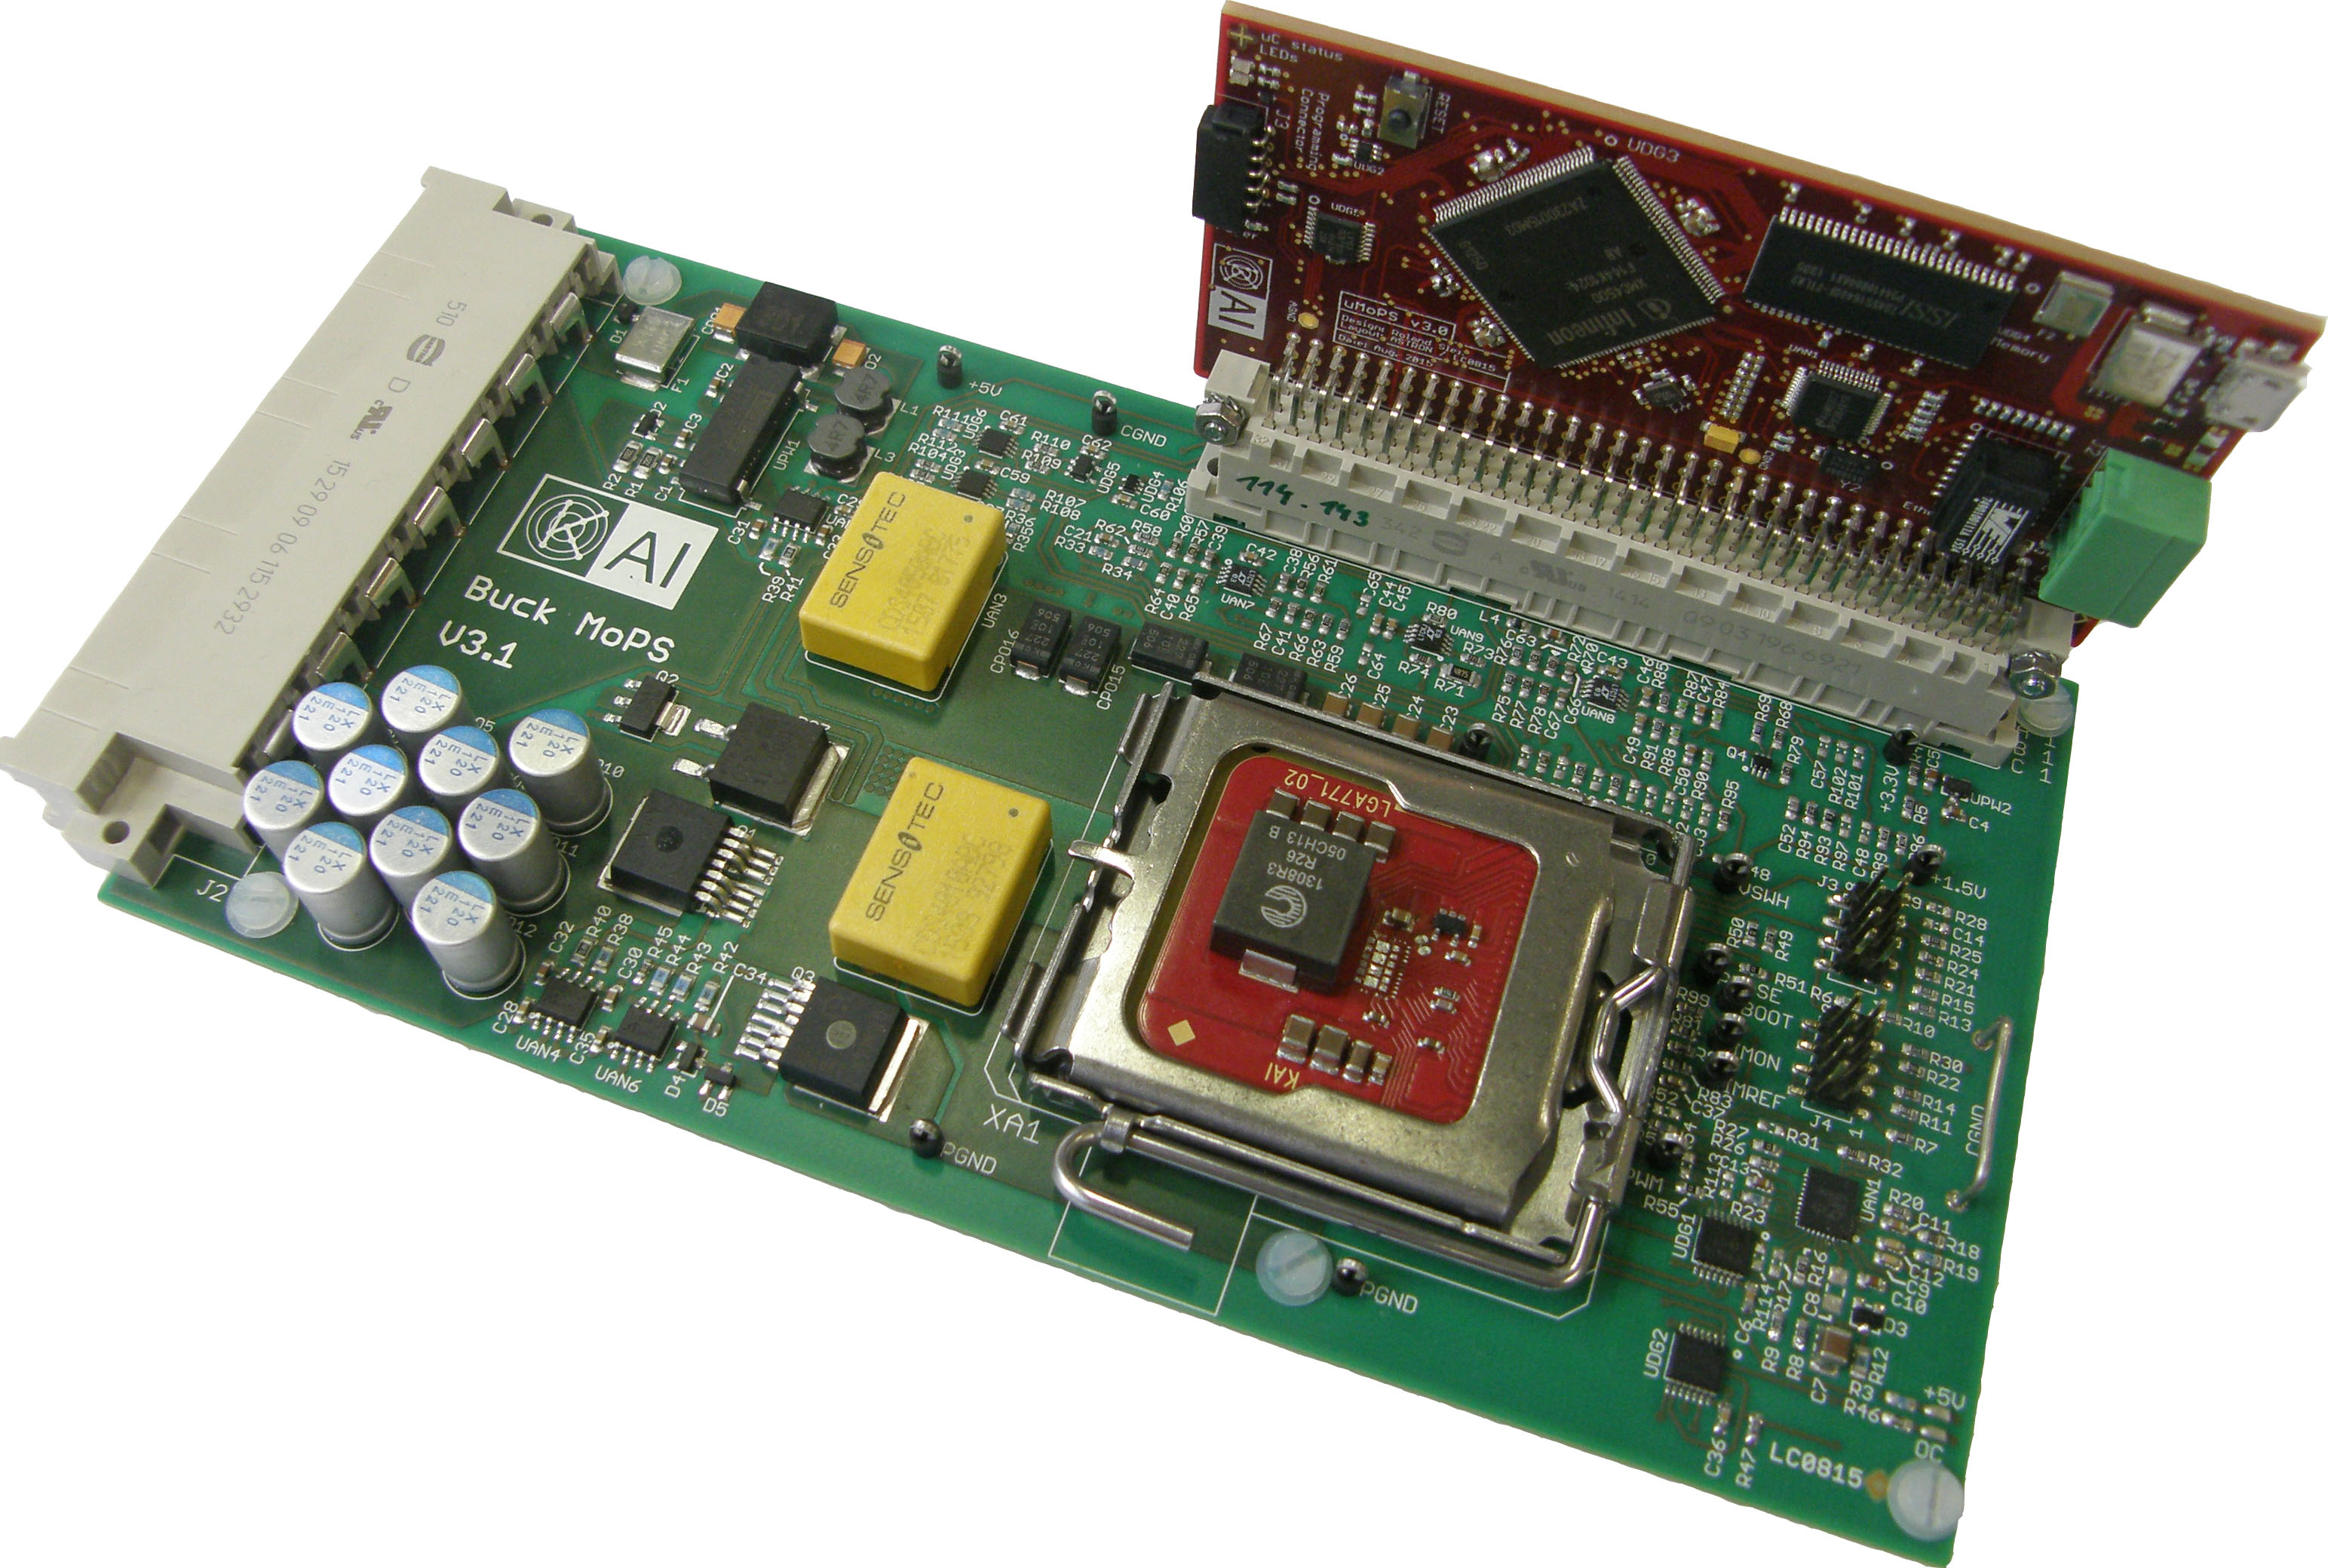
\includegraphics[trim=0 0 0 0, clip, width=100mm, scale=0.75]{images/Buck_and_uMoPS_2.jpg}
	\caption{MicroMoPS, BuckMoPS and LGA771 arrangement.}
	\label{fig:combination}
\end{figure}

\glspl{SoC} play a prominent role in the leap forward of today's technological evolution.
The ability to perform complex functionalities within a small object created the demand for the extensive need of \glspl{SoC} in almost every semiconductor industry.
\glspl{SoC} are leading to provide smart solutions for the dominant, real-life complex problems because of their intelligent features.
To utilize the benefits of the capabilities of \gls{SoC} and to ensure the operation of such micro computing environments and power devices, it is essential to predict the life span of the \gls{SoC} or \gls{DUT} that helps in determining the reliability to use the \gls{DUT} in the real world embedded applications. 
The determination of reliability of \gls{DUT} involves a classical procedure of introducing the semiconductor into various stress scenarios.
From the obtained behavior to predict the \glspl{SoC}' lasting capabilities and reliability.
This is a very essential procedure for semiconductor manufacturers during the development and release of any new semiconductor products. 
Various types of stress tests~\cite{Sleik2016} are performed to extract the characteristics of the \gls{DUT}. 
These stress tests obey a flexible test approach called the Modular test system.
This test system is split into two instances, namely the host system and the hardware module. 
The hardware module is termed as MicroMoPS in this test environment.
The host system is named as \gls{SAM} and controls the overall test flow and communicates with the MicroMoPS\footnote{MoPS stands for Modular Power Stress}.
Many MicroMoPS units may be connected to the host computer via an Ethernet network.
The host computer forwards the stress pattern to the MicroMoPS and receives preprocessed (digitized and filtered) measurement data application and status information.
The inclusion of the application module between MicroMoPS and the stress subjected semiconductor device is for integrating the test circuit, to monitor vital parameters of \gls{DUT} during test runs as well as to provide protection circuits to avoid catastrophic destruction of the test setup in case of a \gls{DUT} failure.
Each application module is connected to one MicroMoPS, which controls the application test, performs measurement data acquisition and logs device status information. 
The application modules are tailored to an individual type of test.
In this work, scaling functions such as Reverse Polish Notation (RPN) and linear scaling are incorporated into the data processing module of MicroMoPS for time and memory-efficient processing of analog measurements. Measurement circuits are analyzed to deduce the linear scaling equation that fits for the data processing system of the Modular test system. Also, the processing of data is automated via \gls{SAM} regardless of the type of stress test application that is performed. The attainment of high speed processing of analog measurements and the automation of processing of data are investigated on a particular stress test type called a Low Voltage stress test system. 
The application module and \gls{DUT} that are associated (\cref{fig:combination}) to the Low Voltage stress test system are termed as BuckMoPS and LGA771 respectively.  
    
\section{Problem Statement and Motivation}

\begin{figure}[htb]
	\centering
	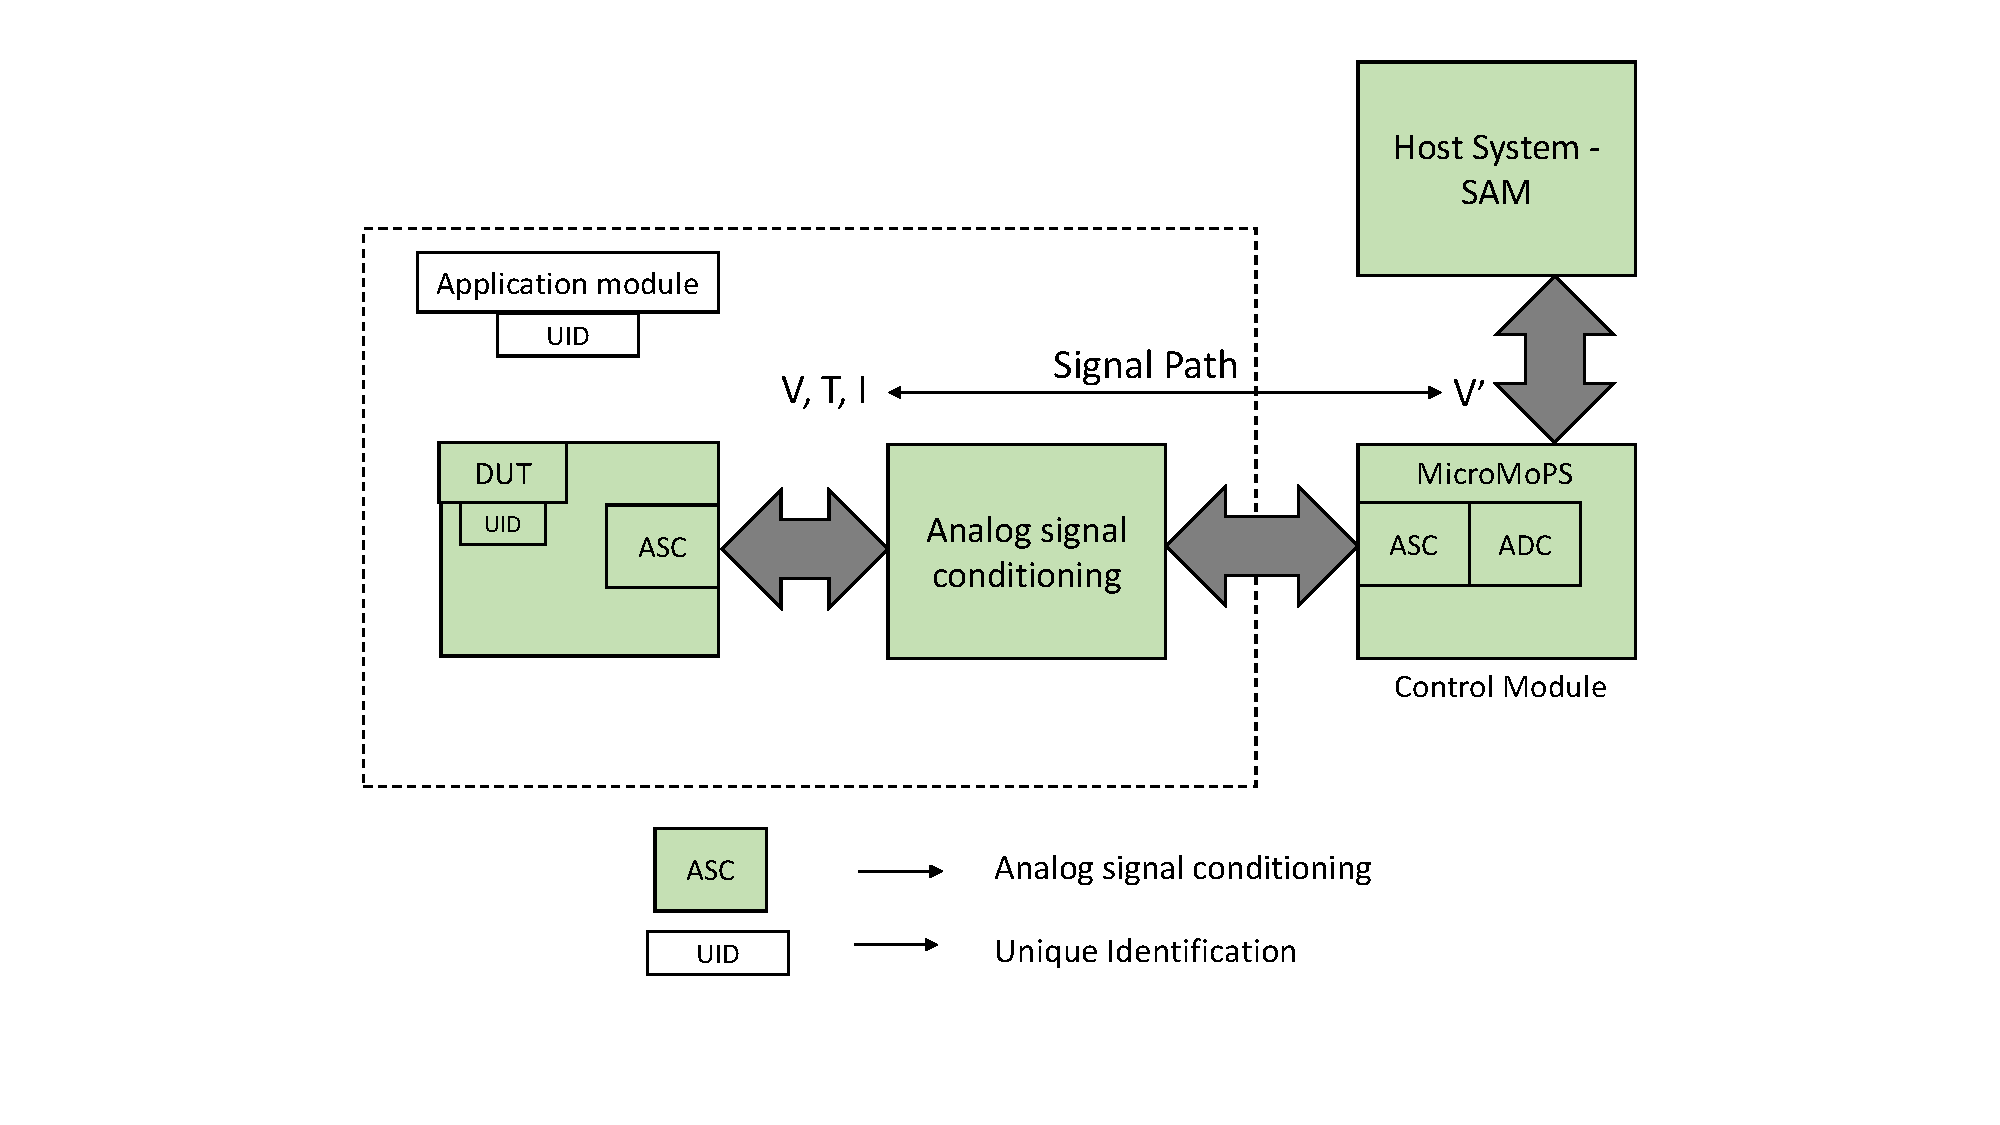
\includegraphics[trim=145 50 0 25, clip, width=\textwidth]{images/High-level signal conditioning.pdf}
	\caption{Measurement environment.}
	\label{fig:Signalmodelmotivation}
\end{figure} 

In this sophisticated test environment, the stress exertion on to the \gls{DUT} is achieved by running so-called \emph{test plans} in MicroMoPS. 
This test plan\cite{Plankensteiner2015} is created by test engineers.
When creating a test plan, it is necessary to initialize all the hardware parameters and test parameters. 
Also, the calculation of measurement related scaling parameters is described in the test plan. 
This method of manual scaling is error-prone and the scaling values may vary based on the type of stress test that is performed. 
Semiconductor devices are subjected to various application specific stress tests~\cite{Sleik2016} such as \emph{power cycling, automotive repetitive short circuit testing, and inductive clamping}. 
In order to avoid manual scaling, the procedure of scaling needs to be automated. 
This way, writing the test plan is simplified and human error possibilities are much reduced.
Using the \gls{SAM}~\cite{Steinwender2016} and the \gls{UID} of application module and \gls{DUT} module, the possibility of automation of data processing is identified.
Another concern is that, the data processing system of MicroMoPS uses a standard scaling mechanism to process the analog measurements~\cite{Sleik2016} into MicroMoPS operating voltage values.
But, from the analog signal conditioning circuit (see \cref{fig:Conditioning}) that lies between the source of the analog to digital converter of control module and source of the analog signal at the application module, there is a scope of deriving a linear scaling equation that processes the digital data in the control module. Introducing linear scaling over standard scaling function improves the speed of processing of analog measurements that are generated on \gls{SoC}.
Also, in a few other scenarios, the scaling function need not have to be linear because of the complex analog signal conditioning circuit that could exist in the measurement environment. To address this scenario, a memory-efficient mathematical notation called \acrshort{RPN} is introduced to the data processing system of the control module.
Hence, the linear scaling mechanism and \acrshort{RPN} mechanism are investigated for scaling in this work.
%Linear scaling equation is a very simple operation compared to RPN, which opens possibility for much more real-time efficient performance in measurement data acquisition.}
 

\section{Research Questions}\label{sec:RQs}
\begin{itemize}
	\item Is it possible to incorporate a robust scaling function to boost the performance of measurement data processing?
	\item Is it possible to derive a linear scaling equation in the test environment that involves complex measurement circuits?
	\item Is it possible to automate the method of scaling in the test environment?
\end{itemize}

\newpage
\section{Thesis Structure}

The rest of the thesis is structured as follows:

\begin{enumerate}
    \item \textbf{Chapter 2} provides a brief overview of the software tools, programming languages, and hardware peripherals that are used in this work.   
    \item \textbf{Chapter 3} presents the underlying concepts of the Modular stress test environment, hardware and software modules in the test environment, measurement data acquisition and processing concepts of MicroMoPS. 
    \item \textbf{Chapter 4} explores the milestones of this project, analysis of the measurement circuit and the approach at which the milestones are achieved.
    \item \textbf{Chapter 5} explains the performed software implementations concerning to the mentioned milestones. 
    \item \textbf{Chapter 6} describes the results that are obtained from performing this work and some analysis with the existing systems.  
    \item \textbf{Chapter 7} concludes the research work of this thesis and provides some recommendations for future works.
\end{enumerate}

\afterpage{\null\newpage}
\afterpage{\null\newpage}
\afterpage{\null\newpage}
\chapter{Fundamentals}
To perform this thesis, the pre-existing firmware image of MicroMoPS and the host application software of the MicroMoPS are extended.
The extension of the MicroMoPS firmware is achieved by utilizing the associated Integrated and Development Environment(IDE), \Gls{DAVE}, and the extension of host application software is achieved by developing applications in the \Gls{LabVIEW} Actor framework of the host application.
The overview of the relevant software tools, programming languages, hardware peripherals, and scripts that are associated with this work is provided in the following sections:    

\section{Programming languages}

\subsection{Embedded C}\label{sec:EmbeddedC}

This is a programming language which is used most widely to develop microcontroller based applications (low level and high level).
The reason for the usage of Embedded C~\cite{Kernighan1988a} is that programs for embedded systems become more complex. 
The complexity arises from the processor operation where the processors are bound to perform complex functionalities such as analog signals analysis, processing of analog signals by applying filtering algorithms, low level I/O operations, fixed-point operators, usage of different memory spaces.
Syntactically and semantically, Embedded C inherits concepts from standard C along with some real-time programming concerns such as dynamic memory allocation and de-allocation, mutexes and semaphores.

\subsection{Lua}\label{sec:Lua}

Lua is a lightweight, high-level programming language, written in C and utilizes a minimum of RAM while still performing as well as expected.
It is designed to be used as an extension language, which means Lua has no idea of a "main" function.
Instead, it can be incorporated into any C based program to enhance its functionality.
Lua is therefore majorly used for providing customizable applications where for the complex applications, macros and scripts may be integrated using Lua.
Lua is not very verbose but a very expressive language.
The example of a Lua program is as shown in \cref{lst:lua}	

%\begin{listing}[htp]
%	\inputminted[frame=single]{C}{src/lua.c}
%	\caption{Lua example}
%	\label{lst:lua}
%\end{listing}

%\begin{lstlisting}[label=lst:lua, caption=Lua example]
  %foo
%\end{lstlisting}

\lstinputlisting[frame=single, label=lst:lua, caption=Lua example, firstnumber=1]{src/lua.c}
	
As it can be seen from lua example code \cref{lst:lua}, functions can return multiple values.
Lua is a dynamically typed language: variables do not have types; only values do.
Lua also supports object-oriented programming.  
	
	\subsection{LabVIEW}
\glsentryfull{LabVIEW} is a graphical programming environment used for testing, measuring and controlling of any computer based data acquisition.
This software offers a \gls{VI} component, which enables users to create their own application in the form of \gls{VI}s and this application could be interfaced with the microcontroller to acquire, process and store the data. 
Applications in LabVIEW are usually built using well-known design patterns~\cite{Gamma1994a} which allows the developed \gls{VI}s to appear much more organized and flexible to provide software extension.
LabVIEW uses the concepts of object-oriented programming such as classes, inheritance, and encapsulation. These concepts provide advantage to LabVIEW to build any software application since the \gls{VI}s which are created using these concepts help to modify the code in respective VIs and the modification does not affect the other sections of code.
A powerful feature of LabVIEW is the Actor framework.
The Actor Framework~\cite{ActorFramework2012,Mercer2011} is used to design and build scalable multi-actor systems~\cite{Hewitt2015a} to solve problems requiring a high level of concurrency. 

\section{Hardware peripherals}

\subsection{I2C}\label{sec:IIC}

\acrshort{I2C} communication protocol~\cite{NXP-I2C-UM10204-2014} is used in communication between multiple slave devices and one or more master devices.
It is a serial communication interface used for short distance intra board communication.
The data exchange using \acrshort{I2C} must adhere a certain protocol for valid I2C communications.
Data transfers are achieved using a data line \Gls{SDA} and a clock signal \Gls{SCL}.
The bus states that are communicated using the I2C protocol are:  

\begin{figure}[ht]
	\centering
	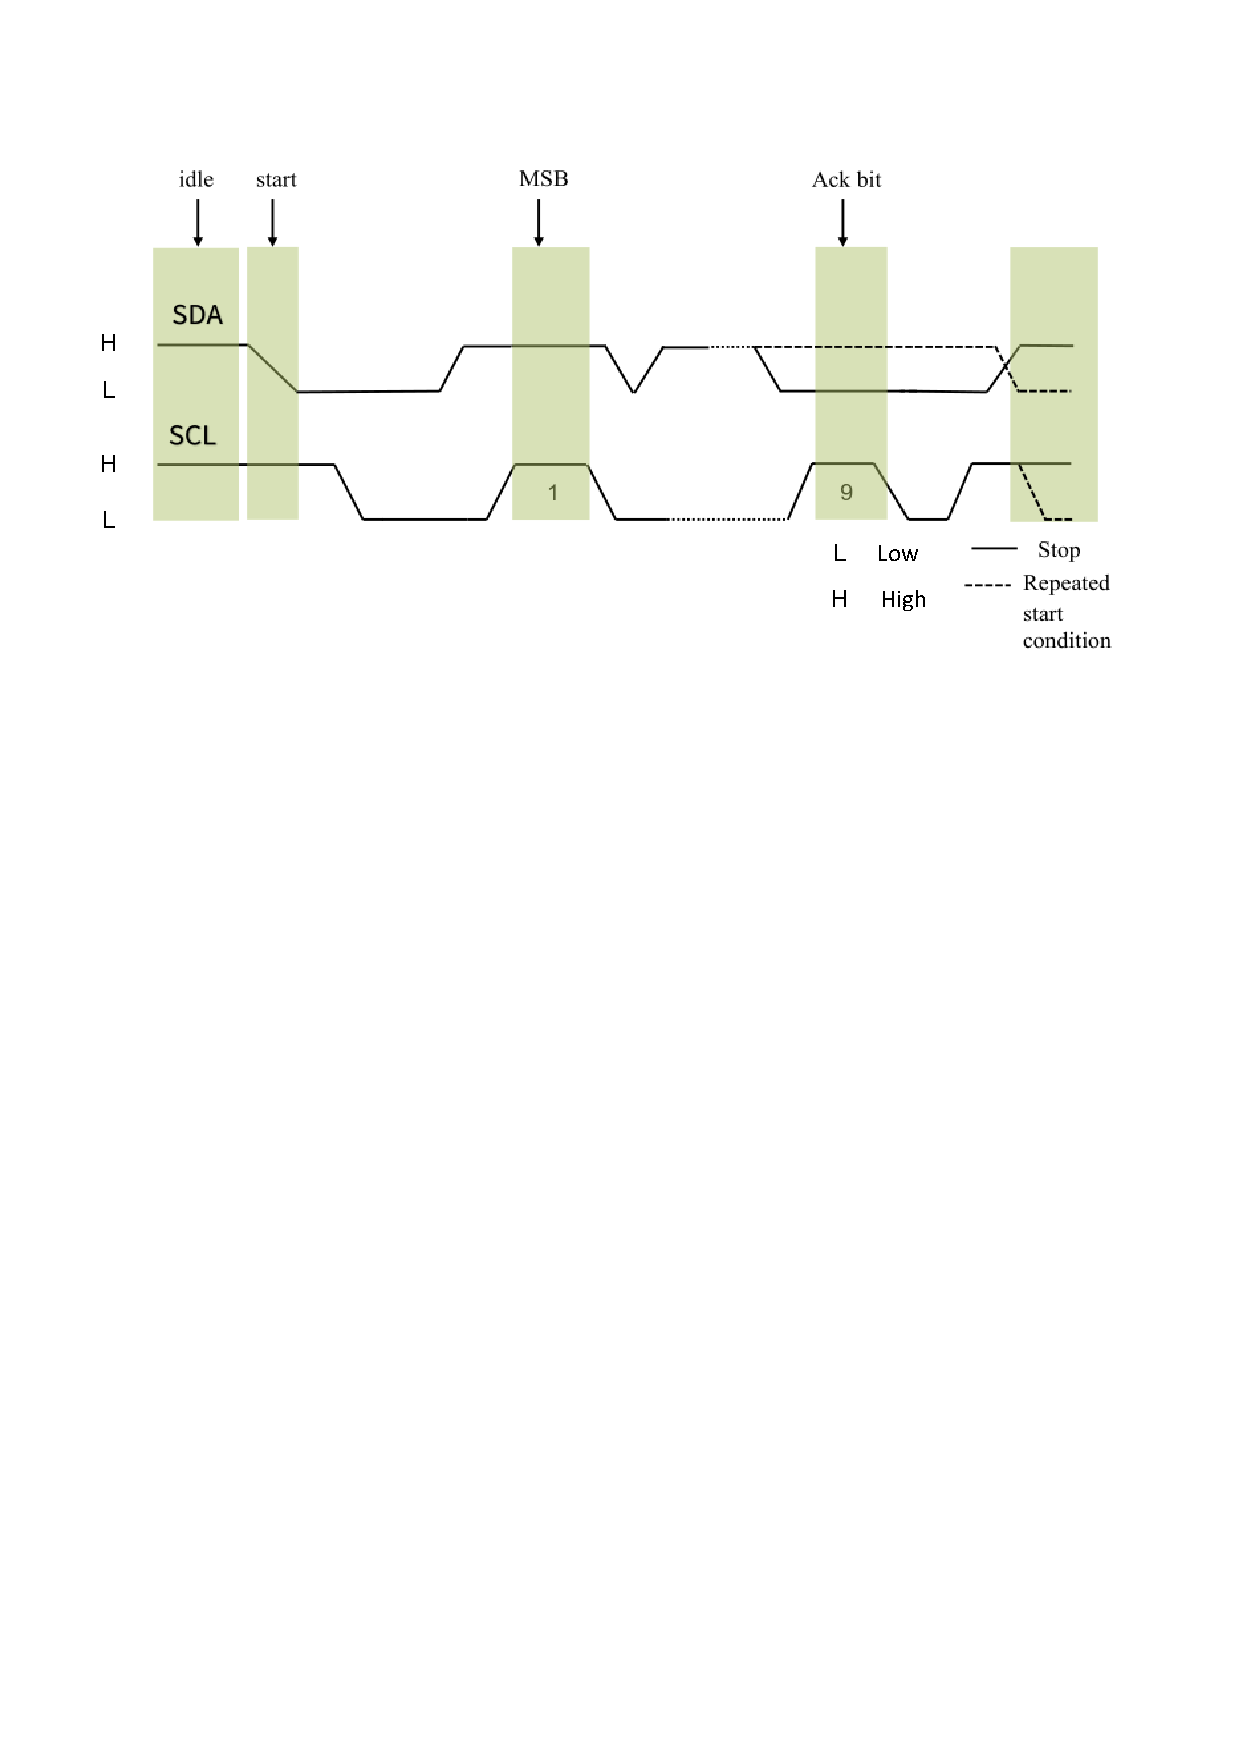
\includegraphics[trim=50 520 60 60, clip, width=140mm]{images/I2C(2).pdf}
	\caption{I2C protocol overview.}
	\label{fig:i2c_image}
\end{figure}

\begin{description}
	\item[Idle] Bus is idle when both, \Gls{SDA} and \Gls{SCL}, are inactive, i.e they are logic HIGH.
	\item[START] START condition is initiated when there is a change in the state of SDA from HIGH to LOW while SCL is still HIGH.  
	\item[Repeated START] Repeated START condition is initiated when there is a transition of SDA from HIGH to LOW while SCL is still HIGH. 
	The master uses this condition to repeat the transfer of data immediately at the end of the data transfer.
	\item[MS bit] The data that the master is intended to transfer is sent in accordance with the generation of SCL pulses. 
	The data on SDA remains unchanged during the entire high pulse of SCL; Transitions of SDA occur only during the LOW state of SCL. 
	Subsequently, data is sent to a receiving device bit wise during the rising edge of SCL.
	As shown in the \cref{fig:i2c_image}, the \Gls{MSB} of data remains unchanged during the first clock pulse of SCL, it follows that the MSB is shifted into the receiving device during the rising edge of the SCL pulse.  
	Likewise, the data is sent bit wise until the \Gls{LSB} of the data is received at the receiver. 
	\item[Acknowledge bit] For every byte data transmission, an acknowledgement bit must be received at the master.
	The master must generate a separate clock pulse associated to the reception of an acknowledgement bit. 
	\item[STOP] A STOP condition is initiated when there is a change in state of \Gls{SDA} from LOW to HIGH while \Gls{SCL} is still HIGH.
\end{description}

Using \acrshort{I2C} communication, data can be read by a master device from slave device.
DS28CM00~\cite{Maxim-DS28CM00-2006a} acts as a slave in this work.
DS28CM00 is a \acrshort{UID} chip that contains \acrshort{UID} of a slave device.
%Steps to read the UID from slave device are as follows: 
%\begin{enumerate}
%	\item Start bit is sent first.
%	\item DS28CM00 is selected as write access from master module i.e. the 8-bit slave address is sent as data using SDA line from master module.
%	 Slave address is unique for different devices. As, per the device information provided in DS28CM00 data sheet~\cite{Maxim-DS28CM00-2006a}, the slave address of the device DS28CM00 is "0xA0". 
%	In this slave address, the least significant bit is set as "0" in order to write the data onto a slave device.
%	\item Acknowledgement bit is received by master from slave, that informs about the status of the data reception.
%	\item The data containing valid memory address (between 00h and 08h) as payload is sent from master, with the direction bit set to 1.
%	The address pointer determines the location from which the master will start reading.
%	When reading from the device, the address pointer increments with every data byte read.
%	\item The repeated start condition bit is sent from master to slave to keep the bus occupied.
%	\item DS28CM00 is selected as a read access from the master module i.e the slave address along the direction bit is set to "1" in order to read the data from the slave device.
%	\item Further, to which the data is received byte-wise from master module over multiple communications. The byte-wise received data are concatenated to restore the 64-bit ROM registration number of the slave module.
%	\item The acknowledgement bits are received for every byte wise packet of ROM registration number. 
%	\item Finally, the stop condition bit is sent from master to slave, concluding the read access communication. 
%\end{enumerate}

\subsection{UDP}\label{sec:UDP}
\glsentryfull{UDP}~\cite{Tanenbaum2010} is a Transport Layer protocol~\cite{Day1983} used for low-latency connectionless communication in IP-based networks. Communication is achieved by transmitting information in the form of datagrams from source to destination without verifying the state of the receiver. 
UDP provides two services such as the port number and checksum capability. 
Port numbers are used to distinguish different user requests and checksum is an optional feature that is used to detect errors in the data that has arrived. 

\begin{figure}[hbt]
\centering
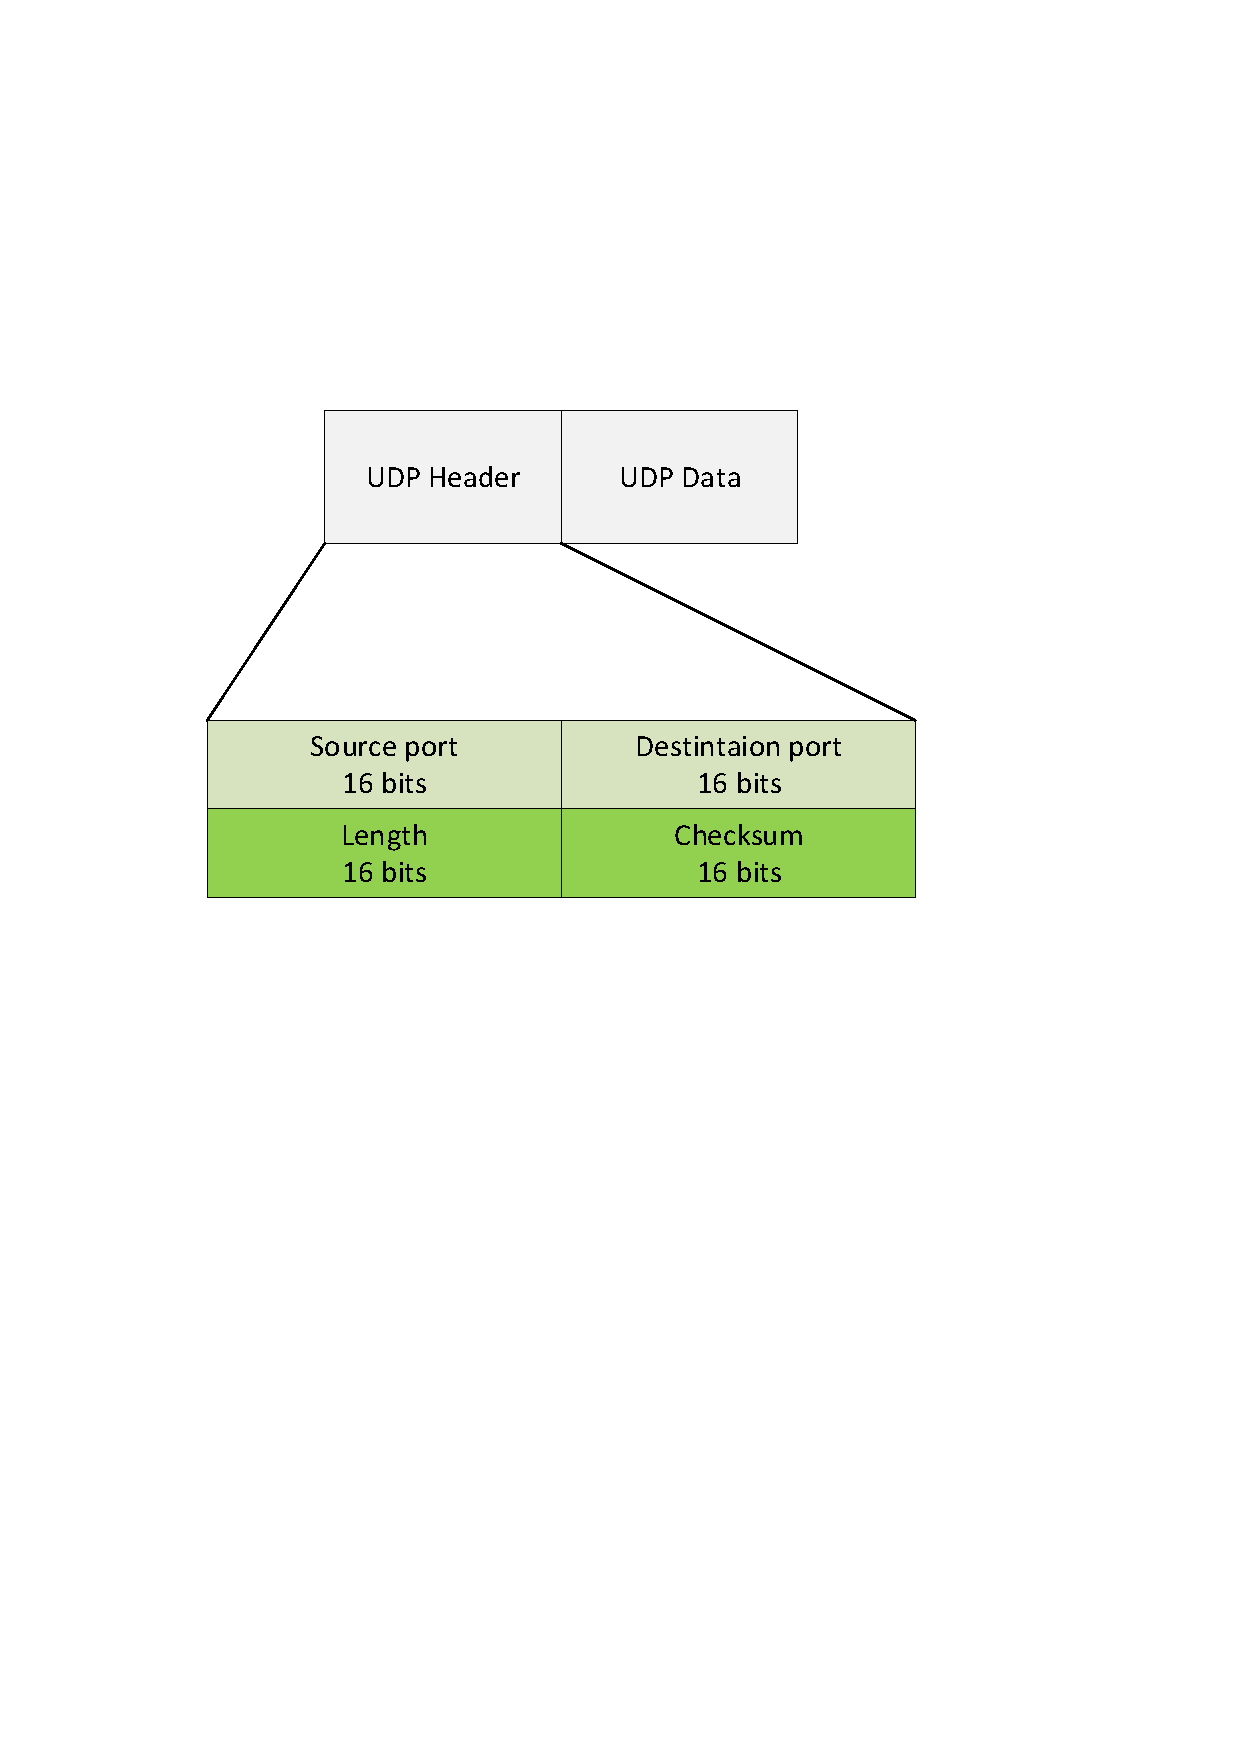
\includegraphics[trim=80 400 150 150, clip, width=80mm]{images/UDP.pdf}
\caption{User Datagram Protocol.}
\label{fig:UDP}
\end{figure}

A \acrshort{UDP} header has four fields, each of these fields is of length 2 bytes. The fields of UDP are:
\begin{itemize}[]
\item{\textbf{Source port}}: The Source port represents the port of the sender.
\item{\textbf{Destination port}}: The Destination port represents the port the datagram is addressed to.   
\item{\textbf{UDP length}}: The UDP length represents the length in bytes of the UDP header. 
\item{\textbf{Checksum}}: The Checksum is used for checking error. 
\end{itemize}

UDP, unlike other transmission protocols, does not use handshaking dialogues to provide a guarantee that data delivers to its destination. 
However, it has very low overhead. UDP works by encapsulating data inside the header field and these data are sent as packets to their destinations. 
UDP protocol is most commonly used as a basic protocol in client-server application protocols such as TFTP, DNS, etc.

\subsection{Analog-to-digital converter}\label{sec:ADC}
Analog-to-digital converter (ADC) is an electronic component~\cite{Rauth2005a} that converts an analog electrical signal (mostly voltage signal) into a digital value.  
Analog signals are the continuous-time and continuous-amplitude signals that could mean physical quantities such as sound, light, temperature, and motion.

Microcontroller consists of an ADC for the conversion of these physical quantities into digital values because microcontrollers can only work with discrete values. ADC follows certain signal processing concepts as shown in the \cref{fig:ADC} in performing the conversion of analog signals into digital values.

\begin{figure}[hbt]
\centering
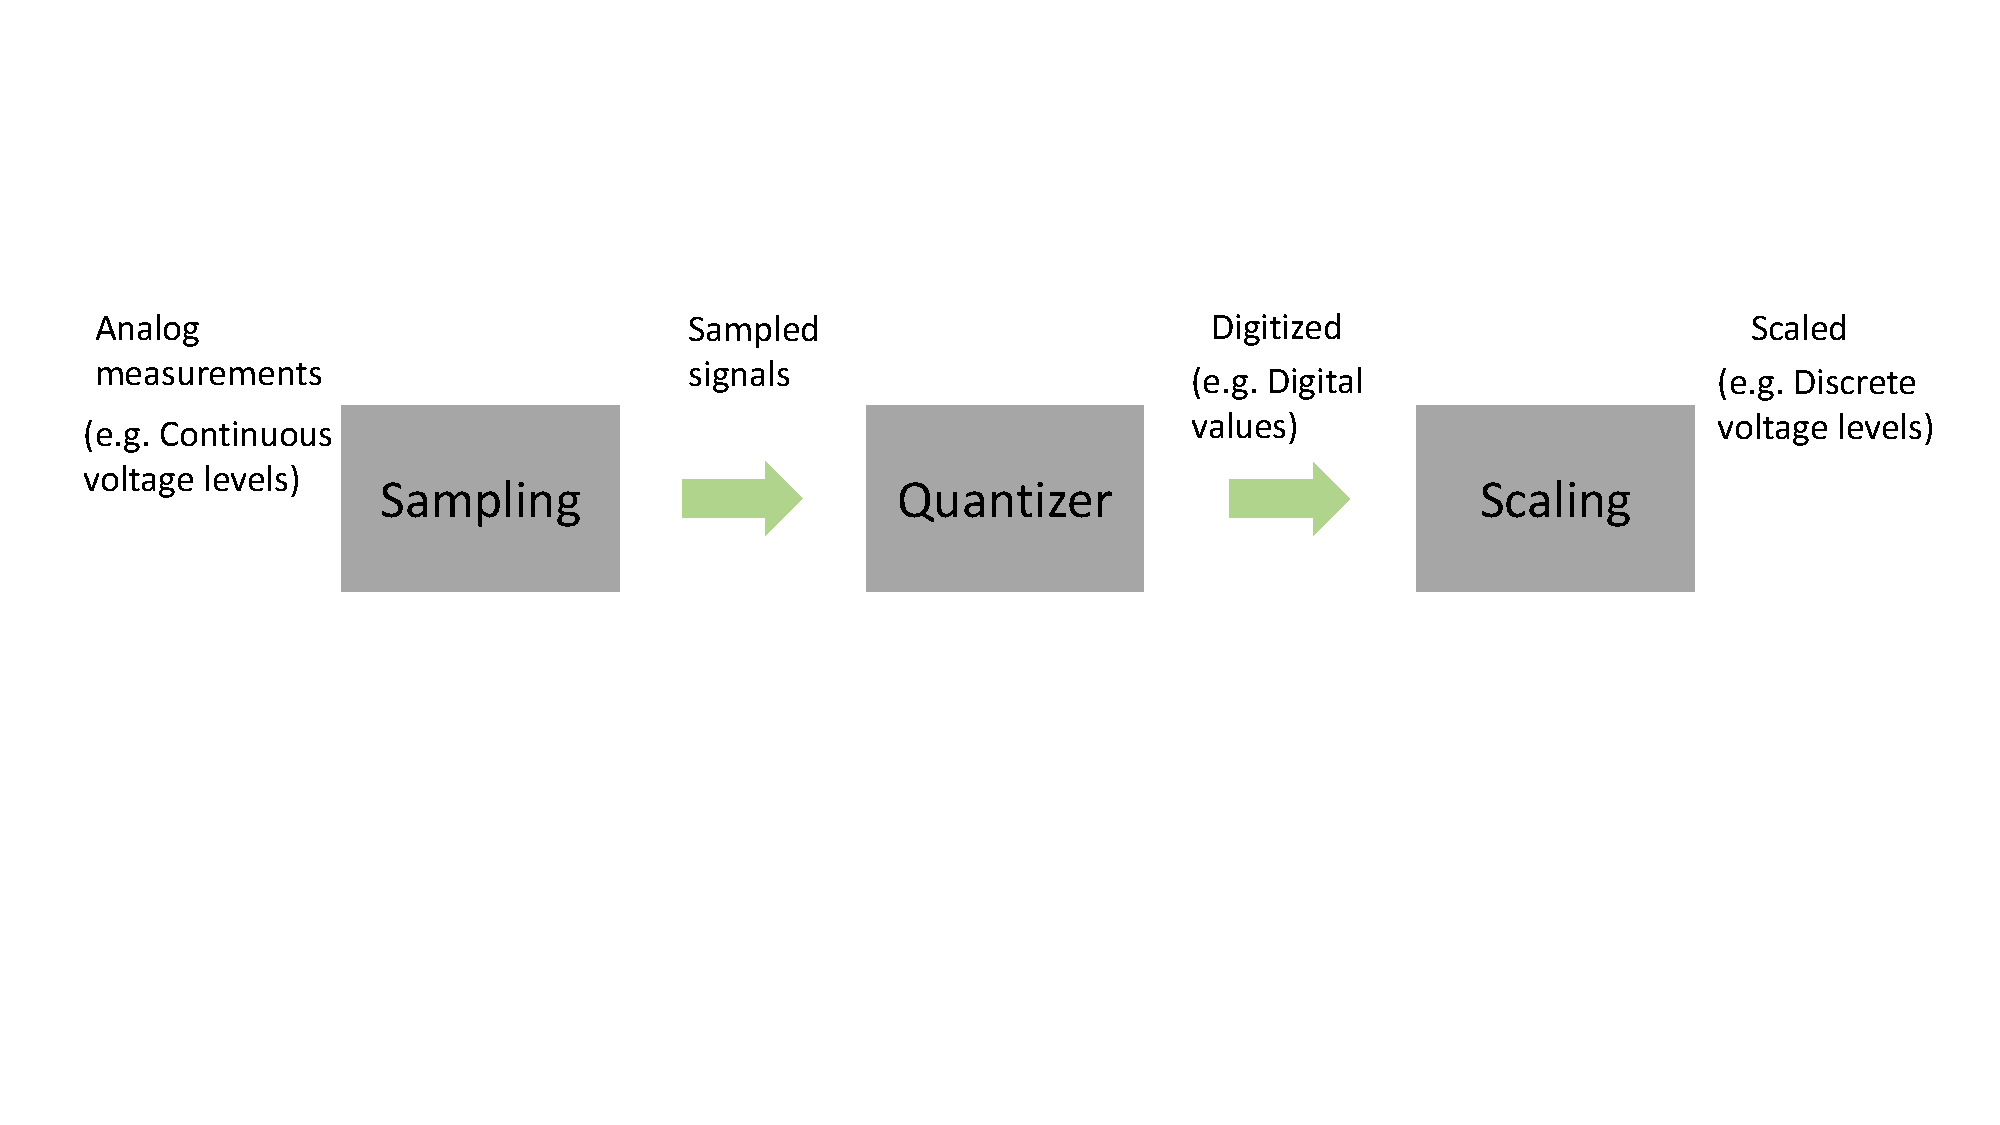
\includegraphics[trim=0 250 25 138, clip, width=150mm]{images/ADC.pdf}
\caption{Sampled Signal.}
\label{fig:ADC}
\end{figure}

\begin{description}
	\item[Signal sampling] Sampling of a signal is performed in order to reduce the continuous-time signal to a discrete-time signal where, any physical quantity such as sound wave or light wave is converted into a sequence of samples. 
	Sampling within an ADC obeys a fixed sampling rate that depends on the input signal, known as sampling frequency (${f_s}$).
	The sampled signal (see \cref{fig:Signal sampling}) is used in the digitization of its every slice. The digitization follows a fundamental principle known as the \emph{Nyquist theorem}~\cite{Miller2010a} to successfully construct a digital signal from the input signal caused by sampling. 
  According to the Nyquist theorem, the sampling frequency needs to be at least twice the highest analog frequency component (${f_{max}}$) of the input signal in order to construct a digital representation. 

The equation that represents the Nyquist criterion is given by:

${f_s} >= 2f_{max}$

  \item[Resolution] The ADC's resolution is the smallest change in voltage that can be detected and thus causes a change in the digital input. This change is also known as the step size of the ADC. The resolution (N) of the ADC can be determined by a bit length that is specific to the ADC. An ADC which has 'n' bit digital output provides $2^{n}$ digital values (resolution), i.e.,
\begin{equation}
N = 2^{n}  
\label{eq:Resolution}
\end{equation}
For example, if the digital output is of a bit length of 12-bit for an ADC, the resolution of this ADC is $2^{12}$, i.e., 4096. This also means that for ADC with the resolution 4096, the digital values for each sample of an ADC range from 0 to 4095.  
\item[Scaling] The processing of the digital data into microcontroller specific discrete voltage values is known as Scaling.
Scaling is performed by using the bit length, digital data, and reference voltage information.
  The standard scaling function of an ADC is given by:
\begin{equation}
f(x) = {\left(\dfrac{V_{max} - V_{min}}{N}\right)\cdot d} - V_{min}, \hspace{9mm}  
\label{eq:Scaling}
\end{equation}
\\
\hspace{19mm} f(x) = Scaling function,\\
\hspace{19mm} ${V_{max}}$ = Maximum analog voltage to be converted to digital output,\\
\hspace{19mm} ${V_{min}}$ = Minimum analog voltage to be converted to digital output,\\
\hspace{19mm} N = Resolution (see equation \ref{eq:Resolution}) of the ADC,\\
\hspace{19mm} d = digital value.
\end{description}
%Scaling function = \frac{V_{ref}}{d} N,


\begin{figure}[hbt]
\centering
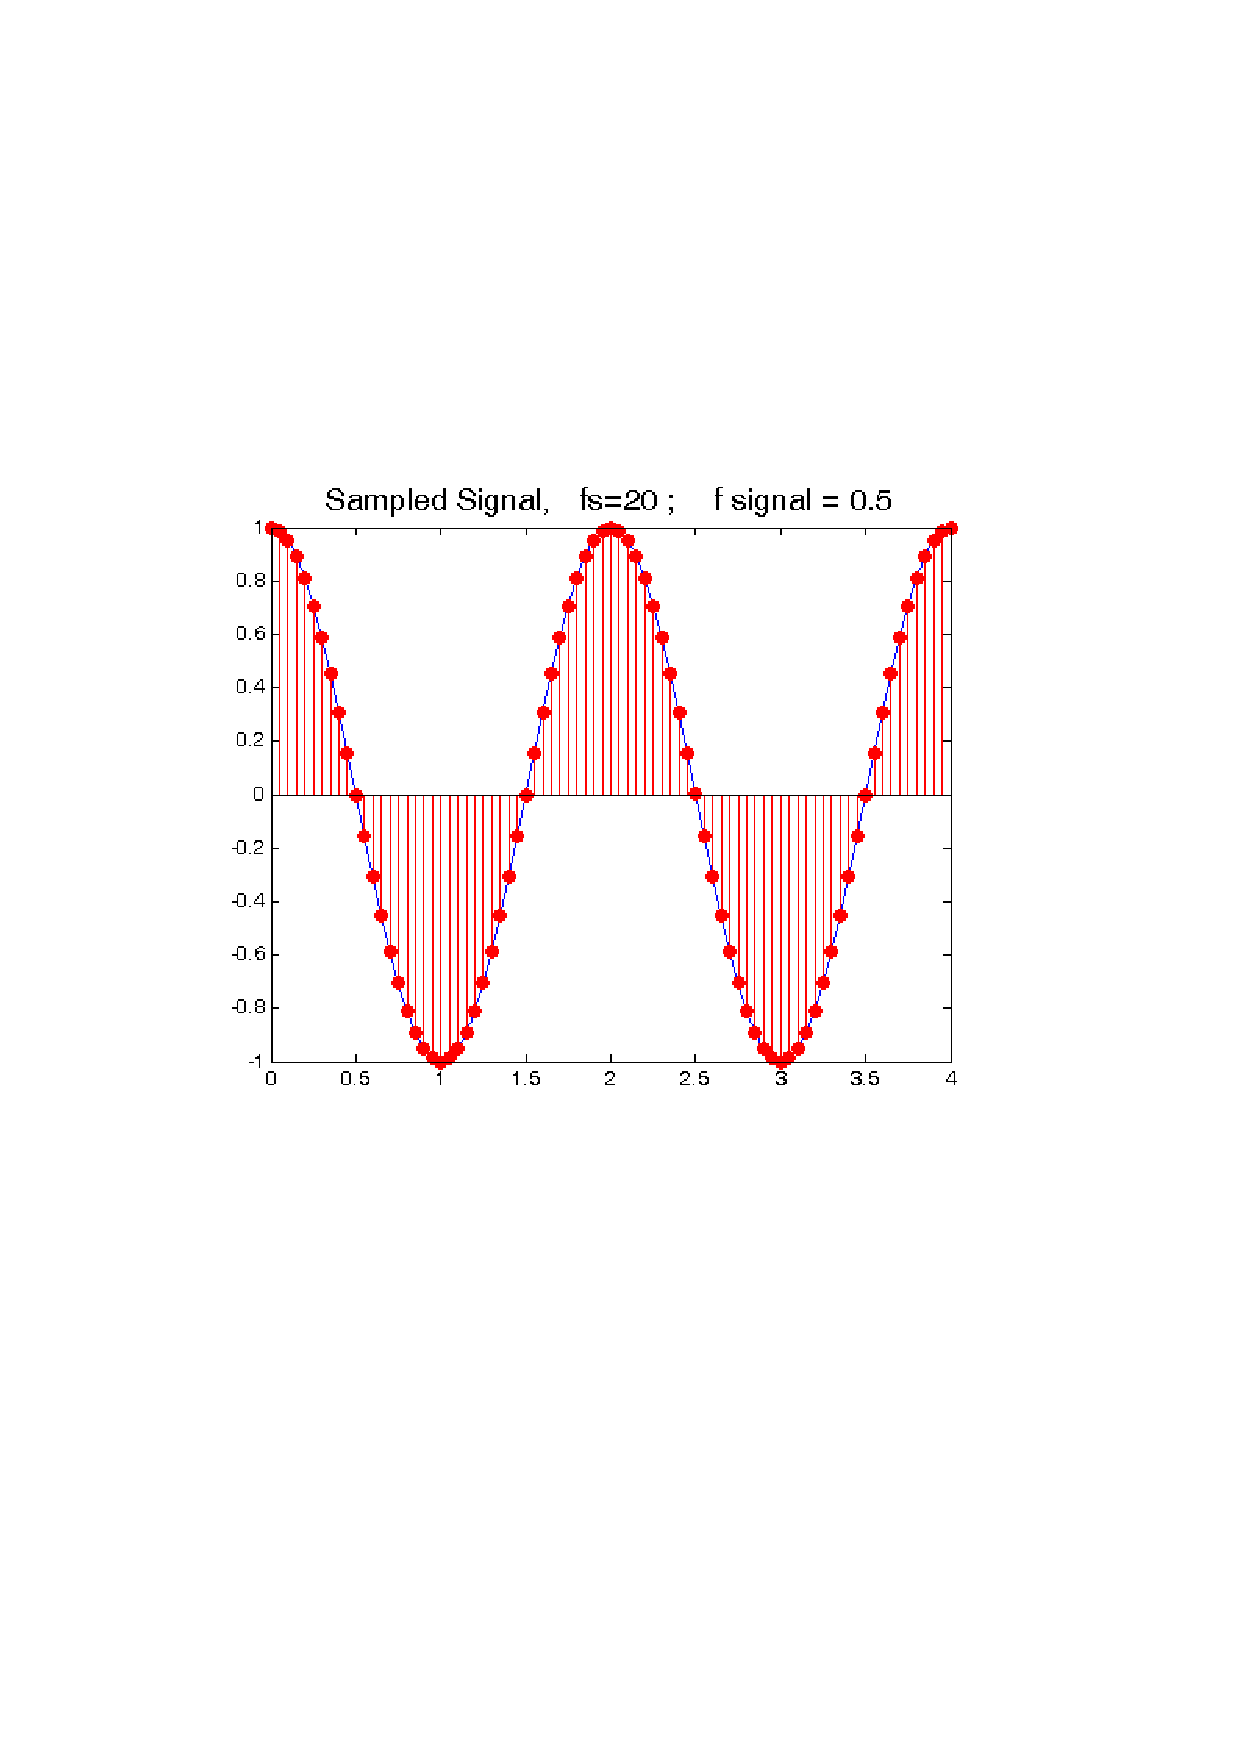
\includegraphics[trim=110 320 100 248, clip, width=80mm]{images/Sampled_signal.pdf}
\caption{Sampled Signal.}
\label{fig:Signal sampling}
\end{figure}



\section{Tools}
	\subsection{DAVE}\label{DAVE}	
			\Gls{DAVE}~\footnote{\url{https://www.infineon.com/dave}} is an Eclipse based IDE using the GNU C-compiler, designed for firmware development of ARM-based 32-bit XMC Infineon processors.
Using the C/C++ language, firmware is developed. 
			\Gls{DAVE} includes the building blocks of software development such as code editor, compiler, and debugger.
The configuration wizard of \Gls{DAVE} provides an overview over the hardware peripherals, control units, and modules. 
			\Gls{DAVE} provides a graphical user interface and wizard, which gets easy for the beginner to get acquainted with the development tool. 
			\Gls{DAVE}'s interactive user interface provides a configuration window which allows the designer to select and configure a specific product and then automatically generate system initialization code for that product, including its core, memory, peripherals, driver functions, and interrupts.    
			In \Gls{DAVE}, user-specific functionality can be added to the automatically generated code without having overwritten the parts when applying further changes to the microcontroller configurations.
%Figure to include}
	
	\subsection{Git}
		 Git~\cite{Loeliger2012a} is a distributed version control tool that supports distributed non-linear workflows. 
		 It is designed for facilitating the co-ordination between the connected programmers in developing software and, track or reverse the changes that are done in the development stages.
%Figure to include}
  		
\section{Markup languages for data interchange}
\subsection{JSON}
JSON~\cite{ECMA-404-2013} is short for JavaScript Object Notation, is a standard file format used primarily for serialization and de-serialization.
Serialization converts an Object-oriented programming's (OOP) object into a JSON string and de-serializing is to do the inverse operation.
It is represented in key-value pairs and is used widely in web applications to generate and parse data.

\afterpage{\null\newpage}
\afterpage{\null\newpage}
\chapter{Related Work} 

This chapter describes the underlying concepts that are involved in this sophisticated stress test environment and their correspondence in meeting the objectives of this work. 
This chapter explains the stress test procedure that is developed and incorporated at KAI, hardware and software systems that are used for the stress test architectures, the measurement \Gls{DAQ} system of MicroMoPS, the scaling mechanism that exists for processing the acquired measurement data, communication channels' specific analog signal conditioning circuits and their role in the acquisition of measurement data.

%{\section{Basic stress inducing principle}}
 
\section{MTS architecture}\label{sec:MTS}
		\begin{figure}[htb]
		\centering
		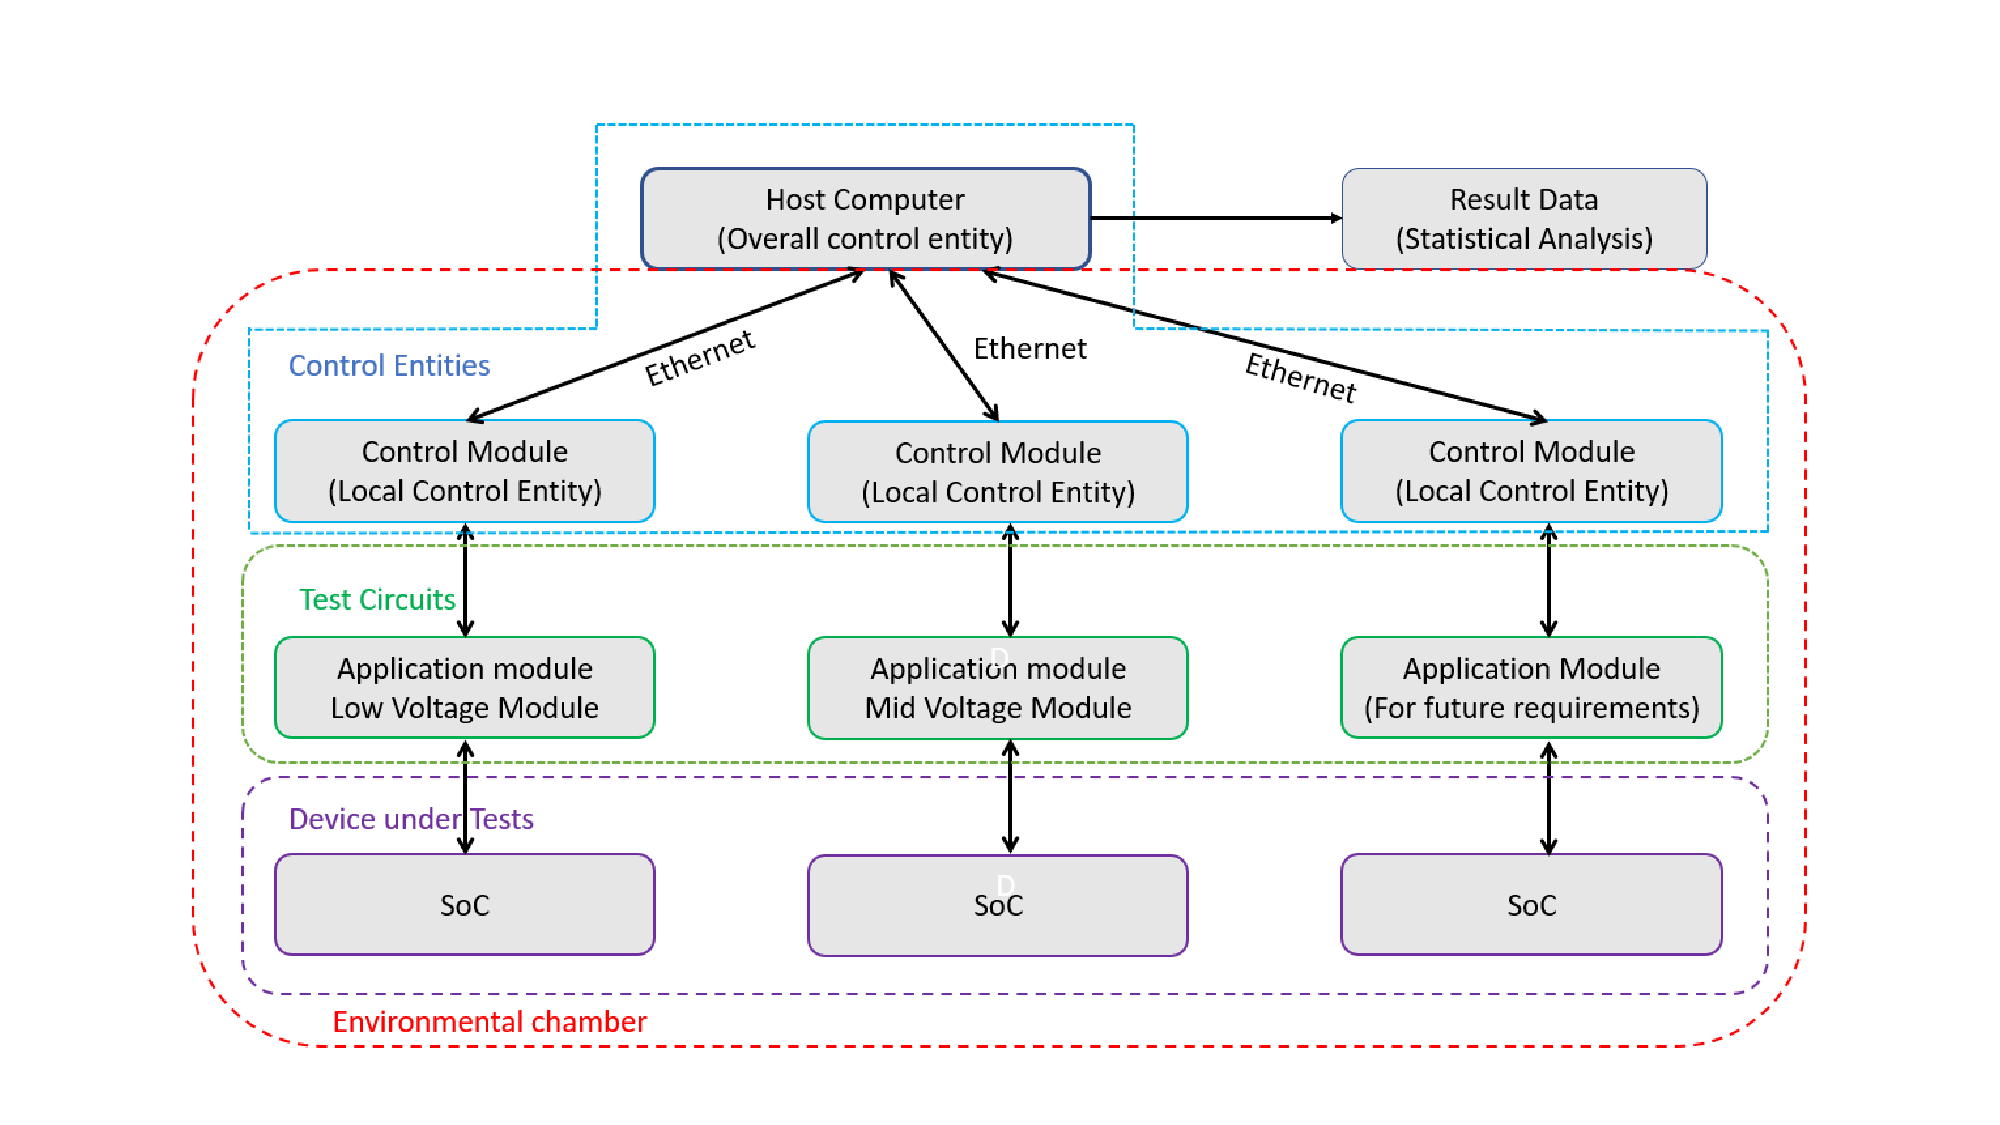
\includegraphics[trim=80 0 0 0, clip, width=170mm]{images/MTS_architecture.pdf}
		\caption{MTS architecture.}
		\label{fig:MTS_image}
		\end{figure}

\begin{figure}
		\centering
		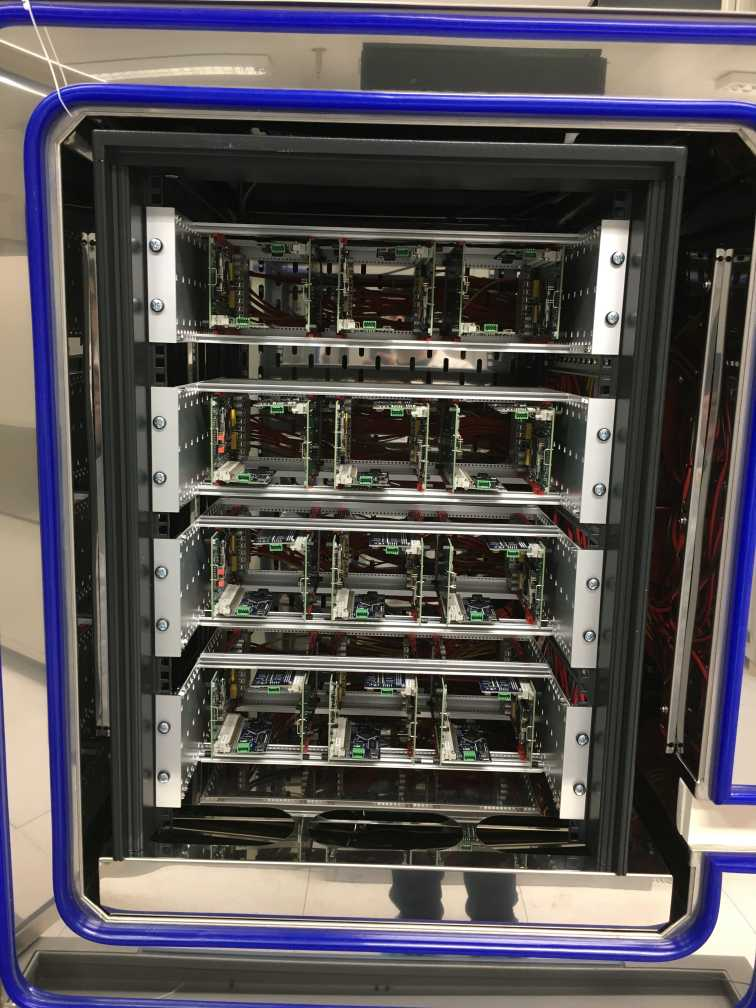
\includegraphics[trim=100 50 0 0, clip, width=65mm]{images/DCDC_System2.jpg}
		\caption{Climate chamber that exerts stress on semiconductor power devices.}
		\label{fig:Climate}
\end{figure}

At KAI, there is a pre-developed modular, flexible and adaptable test system architecture incorporated for reliability stress testing of power semiconductors, which is called \gls{MoPS} architecture~\cite{Steinwender2016}.
This stress test system as shown in \cref{fig:MTS_image} follows a certain flow in delivering a smart approach of executing a reliability stress test on \acrshort{DUT} to estimate their lifetime.
In this stress test system, multiple \acrshort{DUT}s are subjected to stress test patterns under automotive environment conditions.
The MTS architecture is split into two parts, namely the host computer and control module (MicroMoPS). 
The host computer is the central unit system which controls the overall test flow and communicates with the control modules. 
The host computer forwards the test patterns termed as test plans generated by Test Plan Builder~\cite{Plankensteiner2015}. 
Based on the test patterns that are received by control module from a host computer, signals are generated by the control module to provide stimuli to the semiconductor device under test. 
Thereby, the DUT undergoes stress as mentioned in the test pattern. 
The control module further senses the output responses and closes the control loop from a PI controller integrated with the application module, which leads the control module to start recording the measurement parameters of the test. 
The key advantage of \acrshort{MTS} architecture is that there is a total separation of control and measurement part of the test system from the test circuits. 
The test circuits are built within the application module and further, the application module is connected to a semiconductor device under test by a special connector. 
Thus, by the integration of application modules to control modules, it is possible to subject \acrshort{DUT}s into various types of stress tests. 
In order to meet reliability stress testing of power semiconductors under automotive environment conditions, multiple \acrshort{DUT}s and local control modules are attached to the application module and placed inside an environmental chamber as shown in \cref{fig:Climate}. 
These application modules are designed for subjecting \acrshort{DUT}s into specific types of stress test.

Currently, the types of stress tests are:  

\begin{enumerate}
\item Low Voltage Test System: A board called the Buck MoPS is chosen as a \gls{PoL}, which is a DC-DC power converter application. 
The \glspl{DUT} such as power switches are subjected to an application-specific stress test called \emph{power cycling}. 
\glspl{DUT} are heated to reach a temperature between \SIlist{85;125}{\celsius} for consumer devices, \SI{150}{\celsius} for automotive devices and are supplied with a supply voltage that is set to the maximum level which still complies the datasheet specification of DUT. 
Intermittent electronic loads are submitted to \glspl{DUT} which toggle between a high load of {100}{\percent} that nearly reaching \glspl{DUT} to their maximum operating temperature and a low load of \SI{10}{\percent}~\cite{Sleik2016}.  
\item Mid Voltage Test System~\cite{Sleik2018a}: Board such as the \acrshort{PoL} converter is chosen as an application module. 
The \acrshort{DUT}s are power transistors which are subjected to medium voltage stress up to 600V.
\item High Voltage Test System: Devices such as Insulated Gate Bipolar Transistor and \gls{MOSFET} transistors are tested by subjecting to a high voltage of up to 1.5 kV.
\end{enumerate}

The analog measurement data from a DUT is acquired by the data acquisition system of MicroMoPS via the dedicated application module communication channels. 
The analog measurements~\cite{Sleik2018a} such as voltage, current and temperature signals are acquired and go through several stages of attenuation at the application module because of the presence of signal conditioning circuits. 
These signal conditioning circuits are meant for conditioning the measurement data signals into control module specific operating voltage ranges (\SIrange{0}{3}{\volt}).             

\section{MoPS Distributed System}
The Modular Power Stress (MoPS) is a system architecture concept~\cite{Steinwender2013,Steinwender2016} developed to provide a modular infrastructure for customizable stress test applications.
The most essential components of \acrshort{MoPS} system architecture as shown in \cref{fig:MoPS} are: 
\begin{figure}
		\centering
		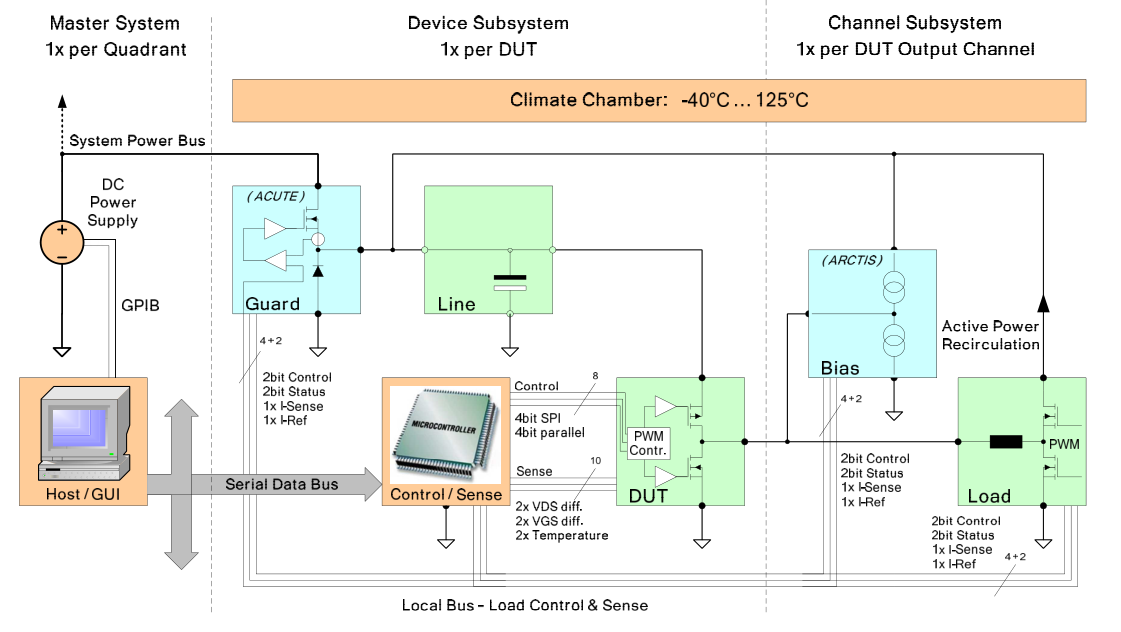
\includegraphics[trim=0 0 0 0, clip, width=\textwidth]{images/MoPS.PNG}
		\caption{Modular Power Stress Distributed system Architecture~\cite{Steinwender2013}.}
		\label{fig:MoPS}
\end{figure}

\begin{description}
  \item[Device subsystem] The components other than control module that are present in the device subsystem act as supporting elements to perform a stress test on a semiconductor device under test. 
  For example, a guard module protects the \acrshort{DUT} from damage by shutting down the power from the control module when there is a device failure. 
  The control module acts as an intermediate agent to trigger application specific stress tests on the \acrshort{DUT}. 
  The control module is situated close to \acrshort{DUT} to establish nearly a lossless one-to-one communication. 
  From the stress tests, the electrical signals that are generated in the \acrshort{DUT} module are measured in the control module via communication channels of the control module.  %And effectively, the local bus(\acrshort{IIC}) is utilised by a control module to detect the UID of associated(better word) application and DUT module. In this thesis, the
  \item[Master system] This is a centralized host, single control entity (see \cref{sec:SAM}) which forwards the stress pattern created by test engineers to a control module (MicroMoPS), to execute stress on the \acrshort{DUT} module. %As, an improvement in exerting the stress pattern to the DUT board, the method of scaling is optimized by including a bit more intelligence to the host computer software i.e SAM, which is discussed in section(refer). 
  \item[Serial Data Bus] This component helps to establish back and forth stress test associated communication between host computer software and the control module. 
  It is also called global bus. 
  Some of the mandatory data exchanges that occur between the host computer software and the control module include: 
	\begin{enumerate}
	\item Reception of test plan by control module from SAM.
	\item Reporting of status and measurement results from control module to SAM via Ethernet. 
	\end{enumerate}
	%Further more set of communications are introduced from this thesis, they are: 
	%\begin{enumerate}
	%\item From this thesis, the UIDs that are detected at the control module, are reported to SAM.
	%\item Based on the UIDs information that SAM has received and oven plan entry given by test engineers(refer test plan builder), respective control module's channels specific scaling value are communicated from SAM to control module, to fit into linear scaling function(refer linear scaling methodologies).
	%\end{enumerate}}
\item[Channel subsystem] The stress test correspondent electronic circuitry namely \acrshort{ARCTIS} is present in this subsystem. An electronic load is driven towards the \acrshort{DUT} via channel subsystem. Also, the real-time controller is part of this system which provides closed loop control logic for the acquisition of the analog measurements.  
\end{description}

\subsection{Hardware architecture}
This section describes the hardware modules of MoPS distribution system.
\subsubsection{MicroMoPS}\label{sec:uMoPS}
The Control module that is used for testing the semiconductor device under test is called MicroMoPS. 
It is a XMC4700~\cite{xmc4700rm2016-RefXMCDatasheet} microcontroller based on the 32bit ARM Cortex-M4 processor core. 
The following are the hardware features that are available in MicroMoPS:

\begin{figure}[htb]
		\centering
		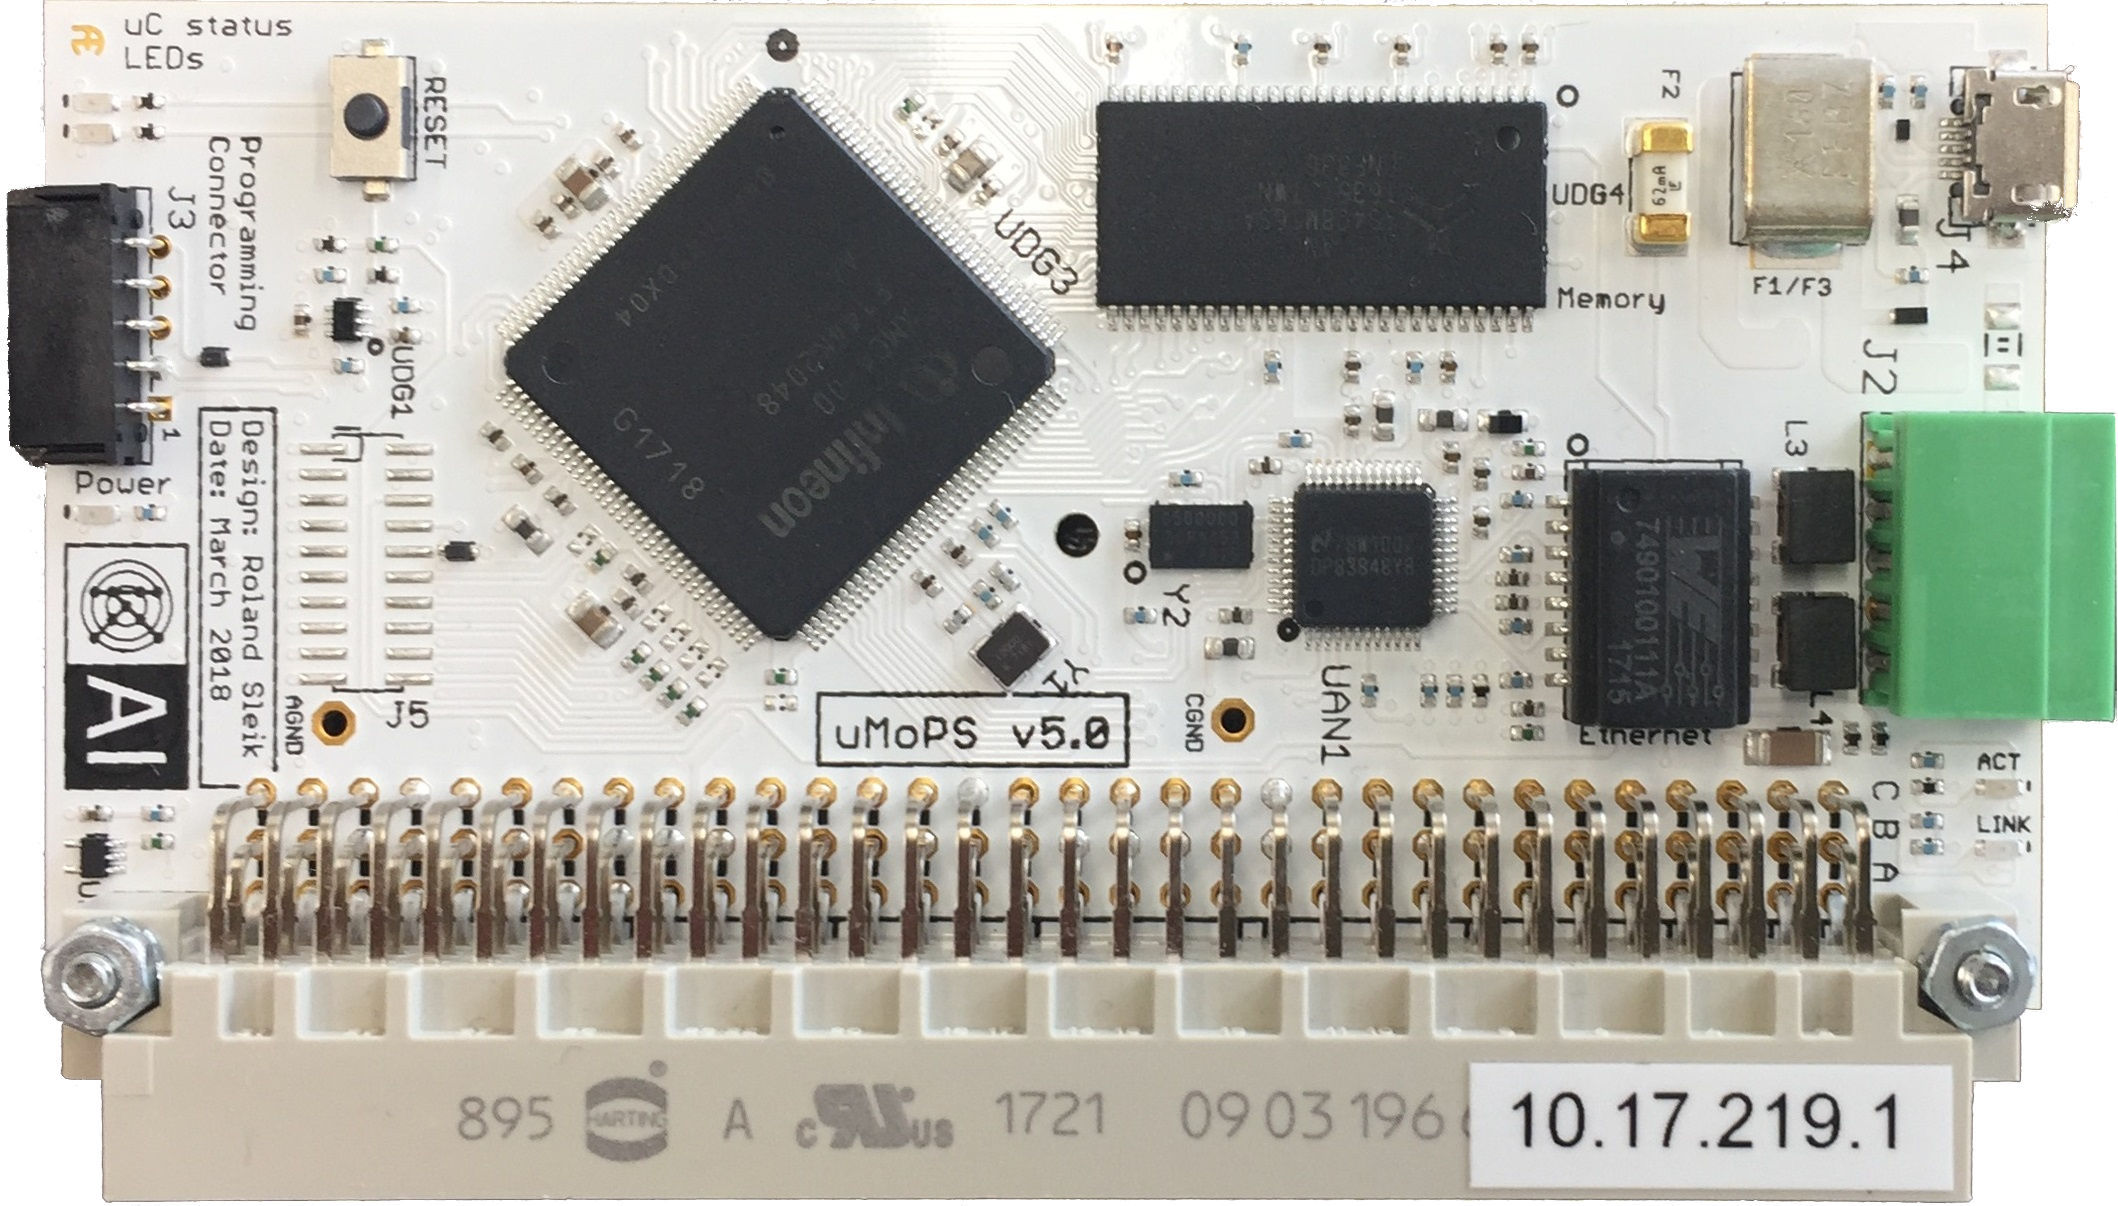
\includegraphics[trim=0 0 0 0, clip, width=120mm]{images/Umopsv5.JPG}
		\caption{MicroMoPS}
		\label{fig:uMoPS}
\end{figure}

\begin{itemize}
	\item Ethernet communication supported with automatic calculation of Medium Access Control (MAC) address deduced from the unique identification number (UID) of the XMC \gls{uC}.
	\item 4 analog input modules capable of acquiring up to 24 input signals with a resolution of 12 bits at rates up to 1.8 MHz.
	\item 4 analog output channels with a 12 bit resolution.
	\item 4 \gls{DSD} channels to gather analog data from galvanically isolated sensors.
	\item 6 \gls{PWM} outputs are divided into 6 units, in which 2 units are provided with an inverted output for half-bridge control.
	\item 1 \gls{SPI} for communicating to a variety of peripherals, such as real-time clocks, memory and control devices such as DAC.	
	\item 1 \gls{I2C} for communicating at low-speed to a variety of peripherals.
			A Key feature of I2C is the capability to control the network of device chips with two \glspl{GPIO} pins.  
	\item 2 \glspl{LED} to indicate run and error states.
	\item 12 \gls{GPIO} pins.
	\item Synchronous DRAM of size 8 MB to store analog measurement data.
	\item Ethernet and \gls{USB} communication interfaces.
	\item Up to 4 software timers of 16-bit width with 1ms resolution for triggering custom events in the test \gls{FSM}.
\end{itemize}

\subsubsection{BuckMoPS}\label{sec:BuckMoPS}
BuckMoPS is the application module which carries the control module - MicroMoPS and DUT - a power switch (IC) to indulge into a low-voltage application stress test system.
BuckMoPS is a DC-DC power stage application.  
The reason behind the addition of an application module together with a control module in the test environment is that it provides a clear separation of stress application from \acrshort{DUT} and control module. 
Also, by introducing an application module into the test system, the \acrshort{DUT}s are subjected to application-equivalent conditions, which helps in the exclusive measurement of power semiconductor device parameters. 
The measurement parameters which are described for the low voltage application stress test system are: input voltage or input current of the \acrshort{DUT}, output voltage or output current of the \acrshort{DUT} and temperature of the \acrshort{DUT}~\cite{Sleik2018a}.   

\begin{figure}[htb]
		\centering
		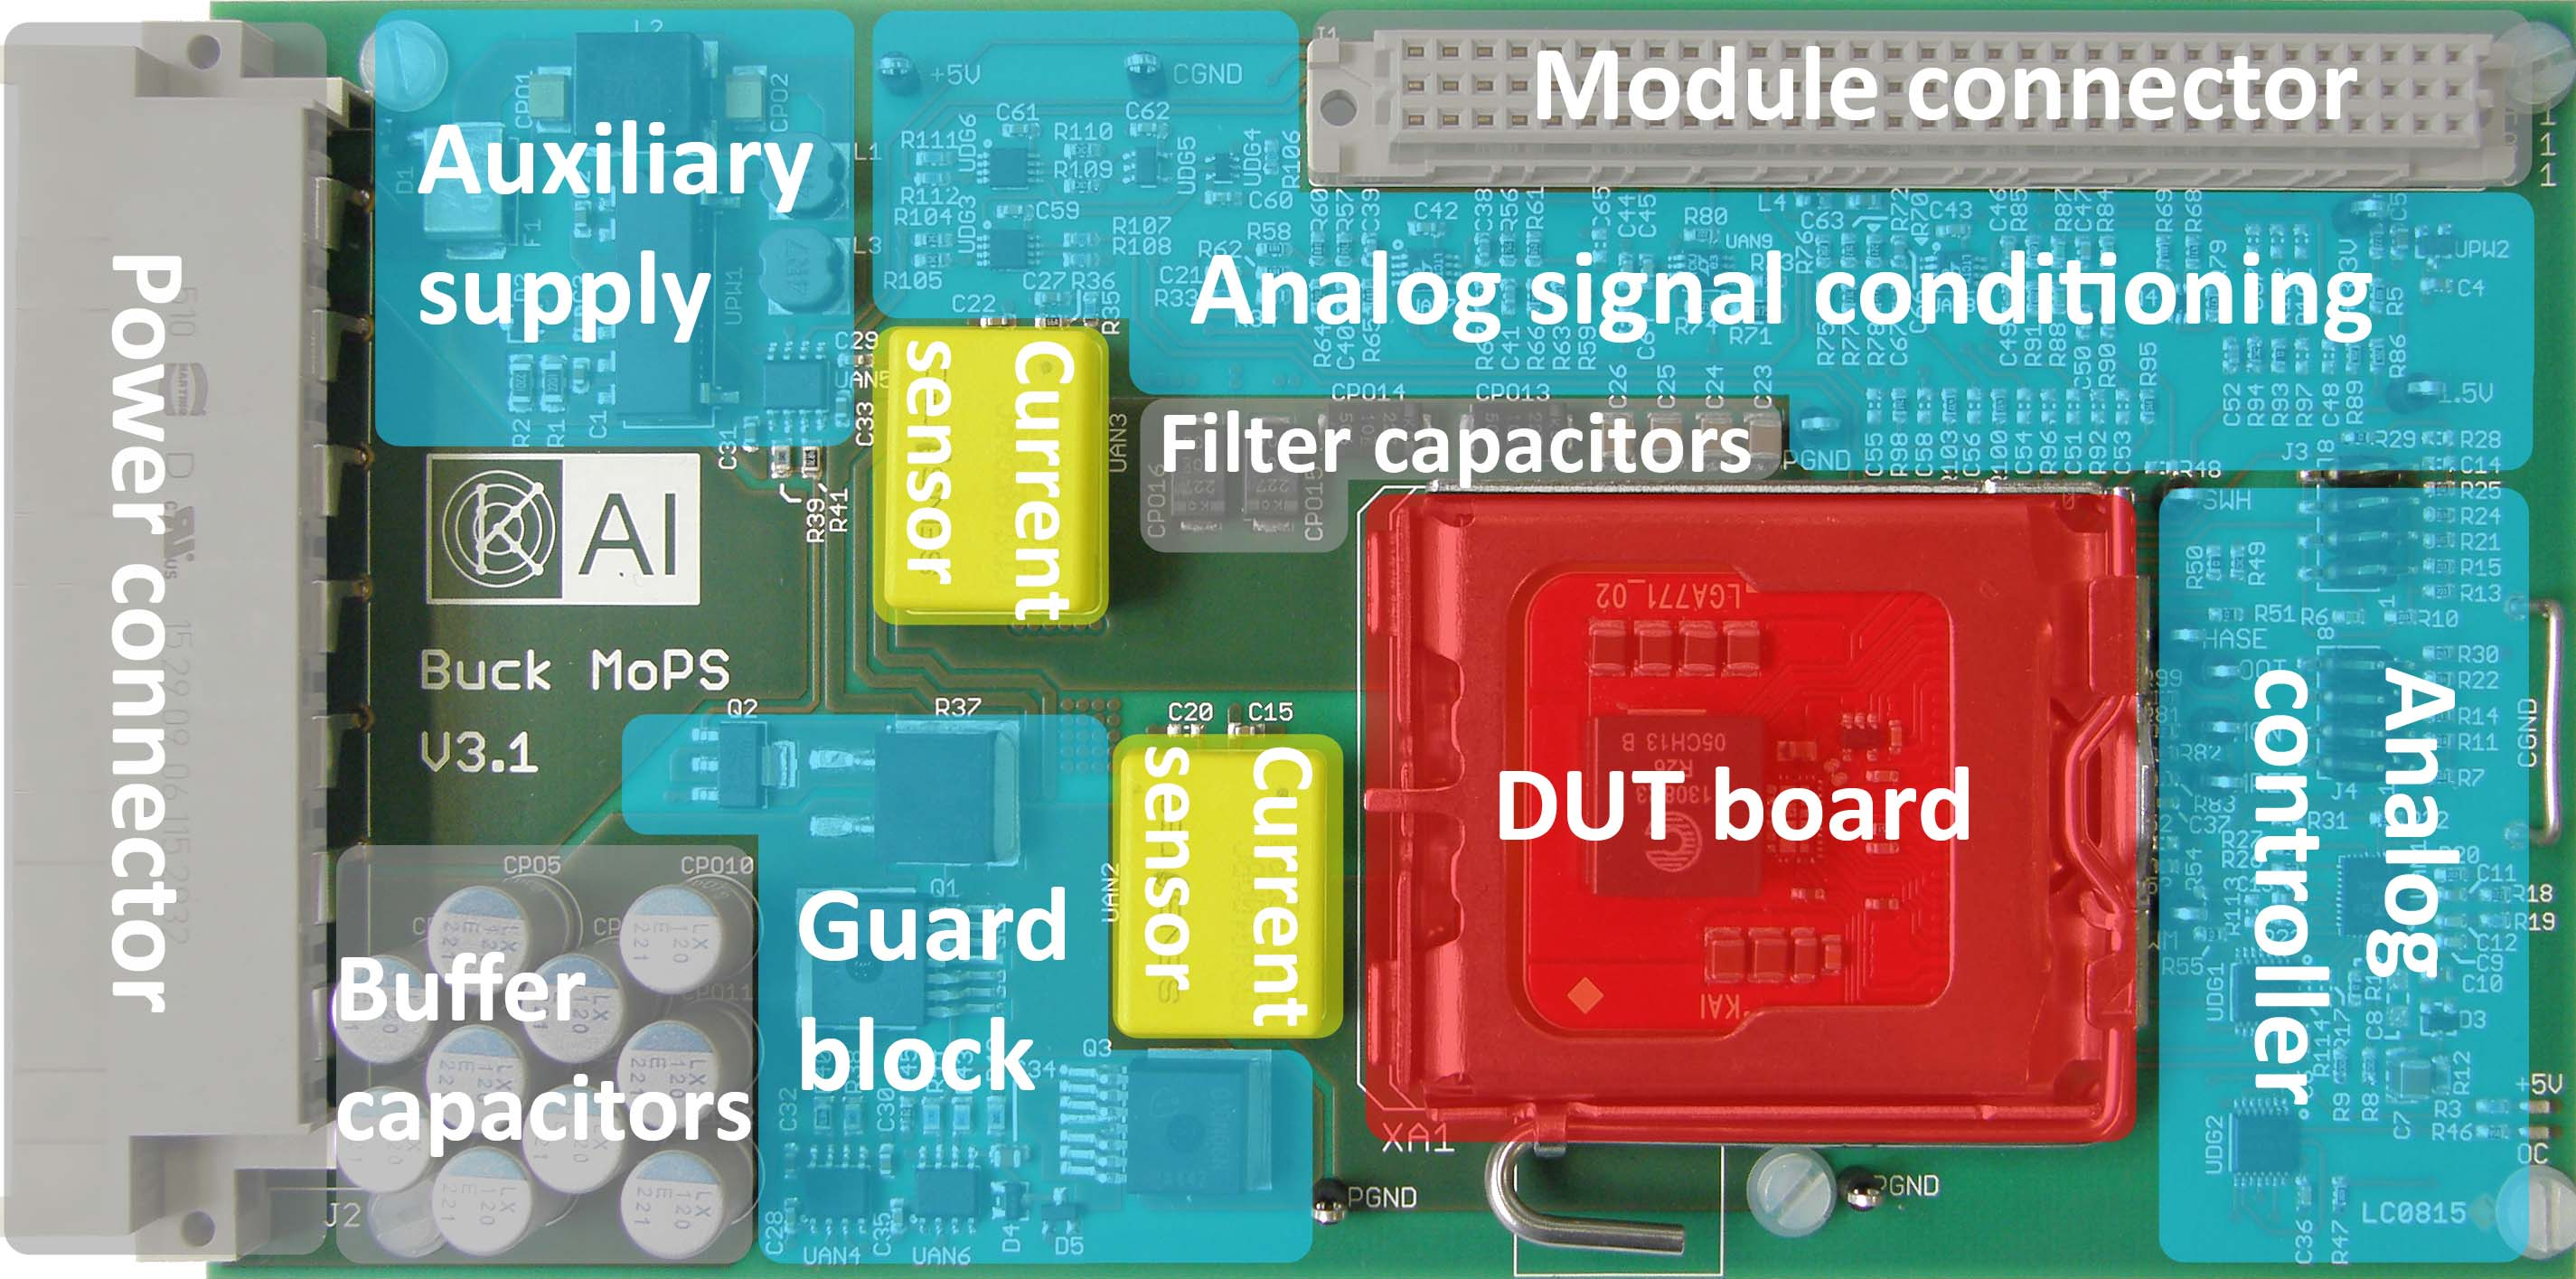
\includegraphics[trim=0 0 0 0, clip, width=\textwidth]{images/Buck_MoPS3.jpg}
		\caption{Low Voltage application board - BuckMoPS.}
		\label{fig:DUT}
\end{figure}

\begin{itemize}[label={}]
\item \textbf{Auxiliary supply:} This module is meant for supplying power to the control module and application module. 
\item \textbf{Guard Block:} This provides smart protection functions that are used to protect the DUT board from over-voltage, which would avoid the damage of the device.
\item \textbf{Analog controller:} This component plays a role in providing a suitable control logic to drive and measure test on DUT board.
\item \textbf{DUT board socket:} This is the area where the DUT board is held and tested.
\item \textbf{Analog signal conditioning:} This component consists of Op-Amps to amplify the signal received from the control module. 
Op-amps are used for conditioning the analog measurement signal i.e. to attenuate analog differential voltage signals into single-ended voltage values that lie within the control module's range. 
\item \textbf{Power connector:} This is the medium by which the power is supplied to application module.
\item \textbf{Buffer and Filter capacitors:} These are useful to support the power supply at high transient events.
\item \textbf{Module connector:} This is the connector that is used to interface control modules.
\item \textbf{Current sensors:} This component is useful for input and output current measurement. 
\end{itemize}

\subsubsection{Device under test}\label{sec:DUT}
The DUT is a pair of \glspl{MOSFET} transistors connected as shown in \cref{fig:BuckMoPS}. 
The Low Voltage application board i.e. BuckMoPS consists of a mentioned \acrshort{DUT}. 
These \glspl{DUT} internally have passive inductors and capacitors to achieve application-equivalent behavior. 
It requires only a \gls{PWM} signal from the control module for the operation of \gls{DUT}.	
\begin{figure}
		\centering
		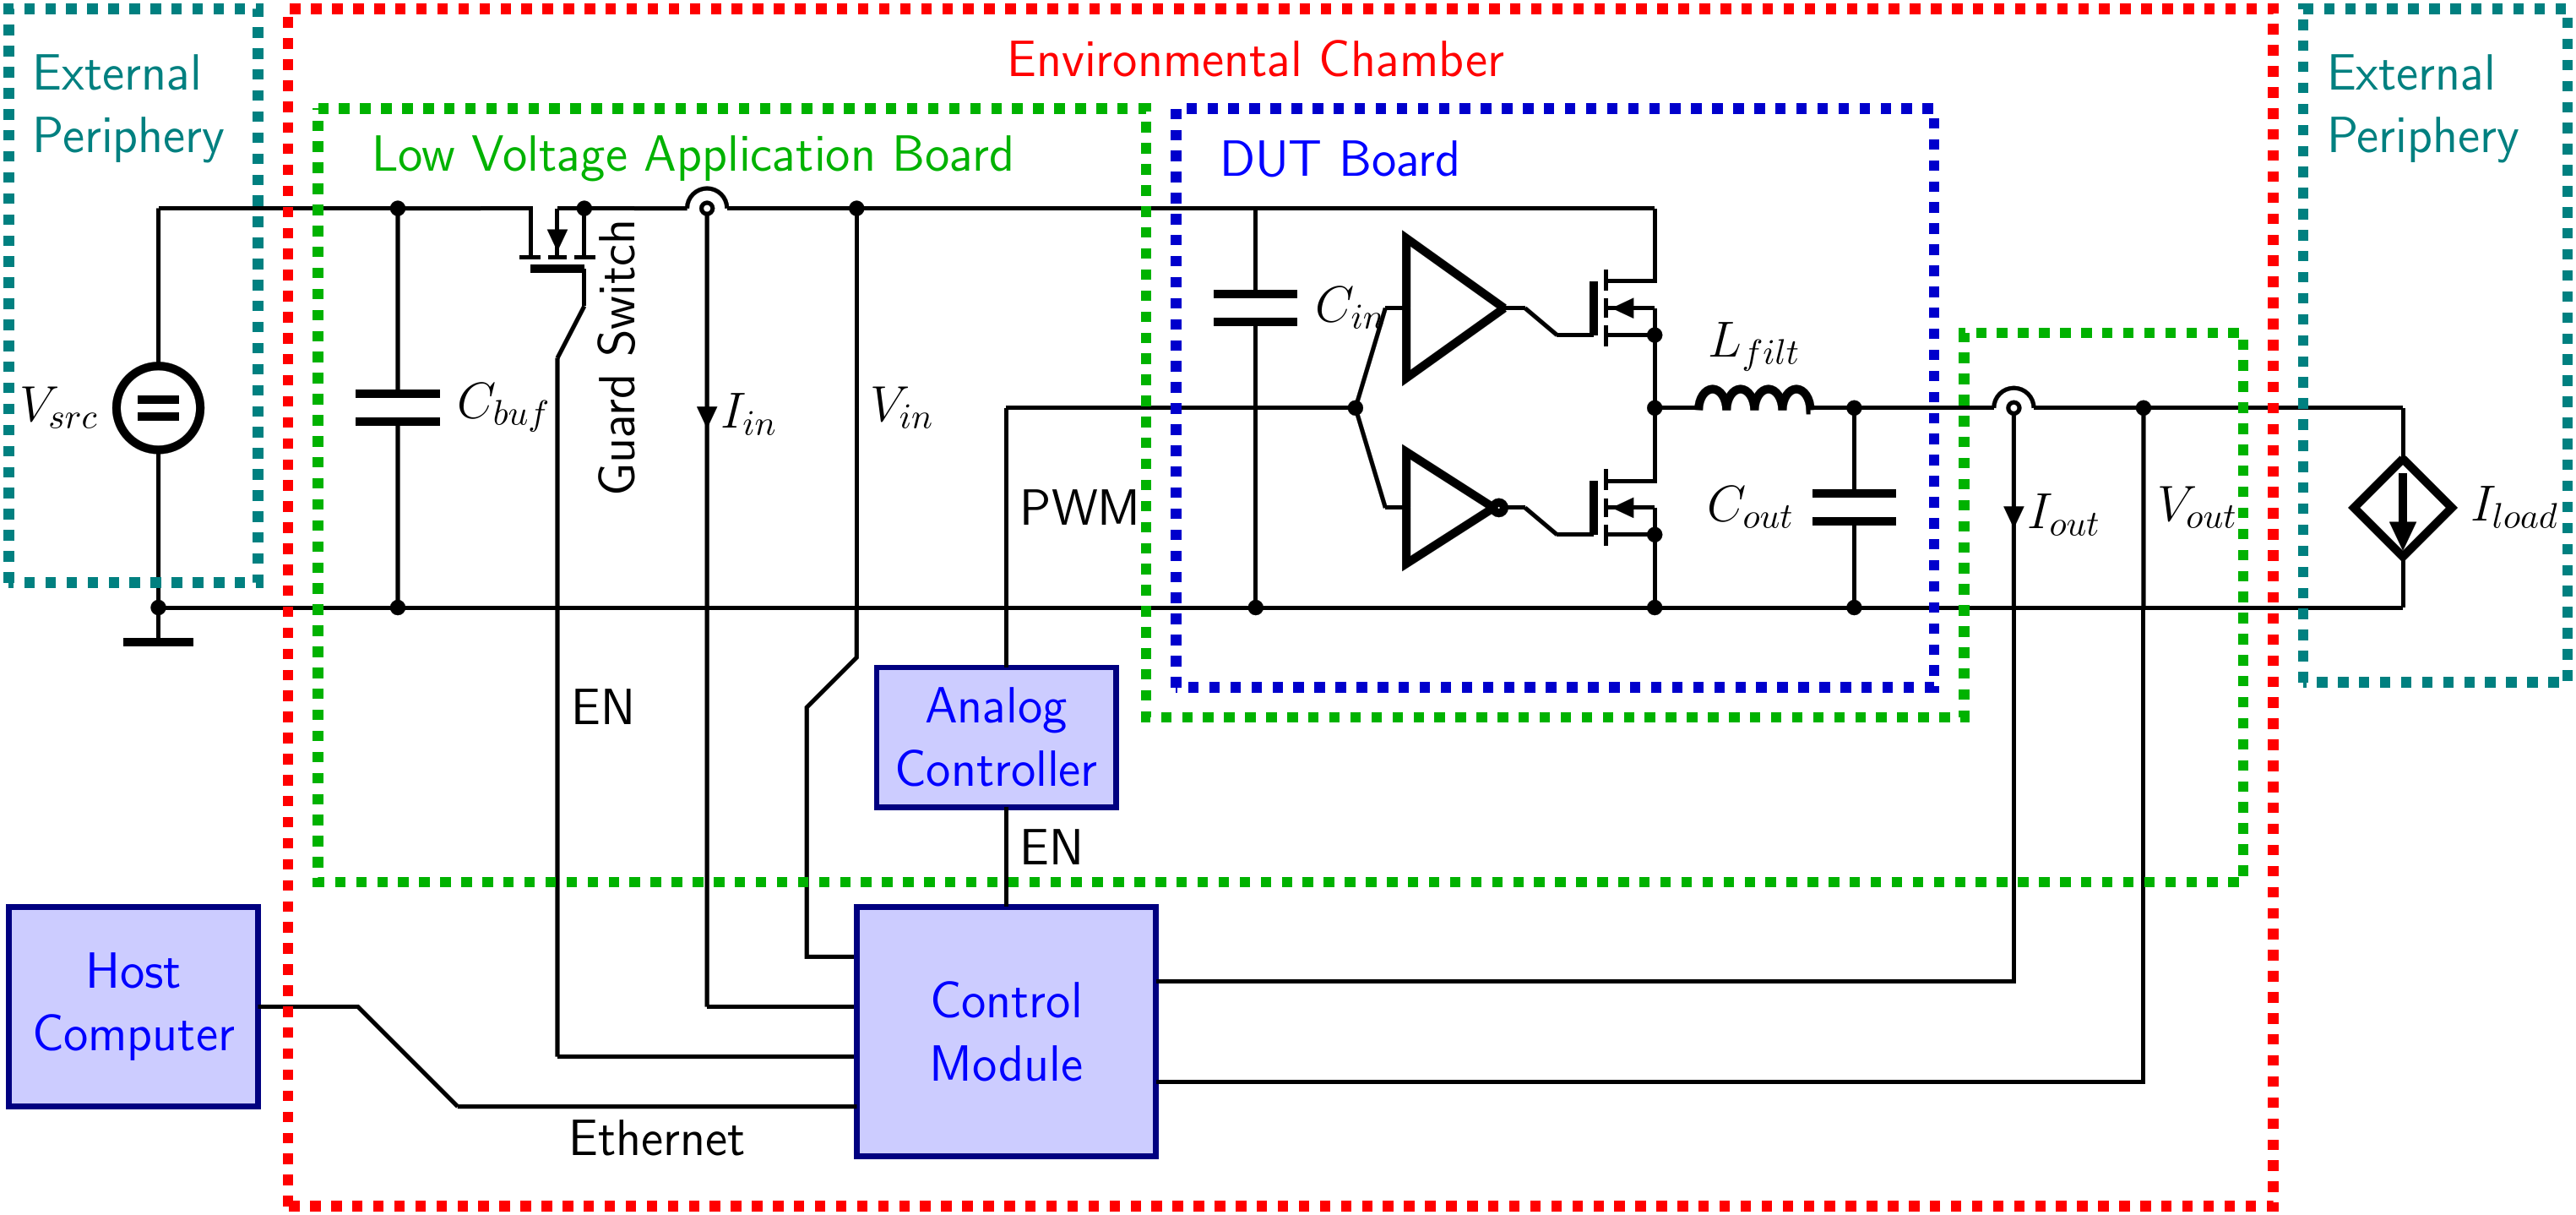
\includegraphics[trim=1370 600 750 100, clip, width=80mm]{images/LV_module_2.png}
		\caption{DUT board plugged to Low voltage application board - BuckMoPS.}
		\label{fig:BuckMoPS}
\end{figure}

\subsection{Software architecture}
This section describes the software layer of MoPS distribution system.

\subsubsection{MoPS-CORE Microcontroller Firmware}\label{sec:CORE}
The MoPS-CORE Microcontroller Firmware is a firmware version of XMC-based microcontroller hardware targets with some CPU resource limitations and memory constraints.
The major handlers that essentially run the entire operation of the MicroMoPS microcontroller are the ones that are included within the main loop. 
By means of measure\_time() handler the time of the main loop is measured for statistical and investigation purposes. 
The handler comm\_handle\_msg() is used in communication between the internal modules of the microcontroller and also to exchange information between the host application i.e. \acrshort{SAM} via Ethernet. 
The handler check\_uplink() is used in testing the connection status between the host and the control module before the test plans are executed on the control module.
Furthermore, the guard\_feed() is a handler that provides a watch-dog guard mechanism, which is a hardware timer capable of resetting the microcontroller, unless it is periodically reset by the software. 
Through the led\_active() handler, the status of the controller is easily detected where there are two \glspl{LED} that are dedicated to give visual indicators to the user about the working state of the controller software. 
Finally, the firmware runs the FSM handler that is developed by test engineers as test procedures and the Lua code that is part of \gls{FSM} diagram is executed to interface the hardware modules of the microcontroller.

%\begin{figure}
%		\centering
%		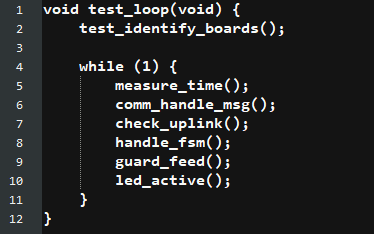
\includegraphics[trim=0 0 50 0, clip, width=100mm, scale=0.75]{images/MoPS_firmware(2).PNG}
%		\caption{MoPS-CORE Microcontroller Firmware}
%		\label{Oven plan window}
%\end{figure}

%\begin{listing}[htp]
%	\inputminted[frame=single]{C}{src/test_loop.c}
%	\caption{MoPS test loop}
%	\label{lst:3-test-loop}
%\end{listing}

\lstinputlisting[frame=single, label=lst:3-test-loop, caption=MoPS test loop, firstnumber=1]{src/test_loop.c}

There are three essential components that are associated to MoPS-CORE Firmware, they are: 

\begin{description}
	\item[Electronic Data Sheet] The \gls{EDS} is the configuration information of control modules that are necessary for performing tests.
	This configuration information includes Hardware version, peripheral information, and device scaling parameters.
	 Fundamentally, the EDS is a JSON string, which is generated upon microcontroller booting. 
	 The microcontroller firmware uses the pre-defined compiled hardware configuration to generate the JSON string. 
	 After the generation of \gls{EDS}, the same is uploaded to the MoPS project web server by SAM so, that other MoPS applications can access the information. 
	%In this work, slight modifications are done in generation of ai MoPS module instance of EDS, in order to facilitate the creation of "scaling.json" in MoPS web server. This "scaling.json" further helps SAM to understand about the expected stress test scenario that needs to be performed and to adjust the scaling parameters in control module to perform linear sclaing. Also, ai communication module of MoPS hardware configuration is extended to enable the operation of linear scaling to process the digital representaion of stress measurements.}     
	
	\item[MoPS web server] The MoPS web server is the server software dedicated for storing Hardware information of the MicroMoPS and delivering Hardware information of the MoPS microcontroller to the corresponding host software application such as TestPlan Builder. 
	 
	\item[Lua interpreter] The Lua interpreter~\cite{Ierusalimschy1996a,Steinwender2015} is to provide flexibility to the hardware designers and product engineers of the company in configuring a test sequence directly without having to deal with the low-level programming of microcontrollers. 
	A set of Lua commands are available to provide a hardware interface and they are simple to use. 
	These Lua commands contain the implementation of custom modules and hardware access routines. 
	They access hardware modules via defined C-APIs. Each Lua command (enclosed within FSM) present in the test plan accesses it's corresponding C-\gls{API} from the Lua space of MicroMoPS firmware and thus, allows the MicroMoPS to execute the entire test plan.
\end{description}


\subsubsection{Software Architecture for MoPS}\label{sec:SAM}
Software Architecture for MoPS is a host layer software~\cite{Steinwender2016} developed using LabVIEW.
This software is designed for test engineers to perform any type of stress testing from their respective host computers.
The stress tests are applied by loading a test plan into SAM software. 
This software makes use of the Actor framework~\cite{ActorFramework2012} of LabVIEW to essentially create multiple independent software agents called as Actors. 
These actors have a separate GUI window displaying their concerned attributes. 
Furthermore, these actors also run some tasks in the background and accordingly their corresponding GUI is refreshed and displayed to provide test engineers a user-friendly interface to interact with. 


\begin{figure}
		\centering
		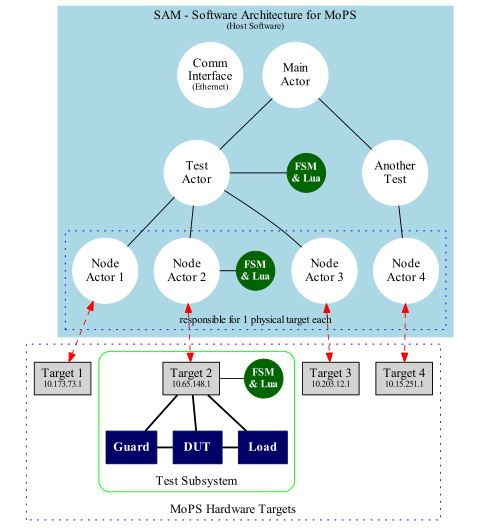
\includegraphics[trim=0 0 0 0, clip, width=80mm]{images/SAM.JPG}
		\caption{Software Architecture for MoPS}
		\label{fig:SAM}
\end{figure}

SAM is organized in a hierarchical manner as shown in the \cref{fig:SAM} where each of these software agents is meant for particular tasks that are fundamentally connected to a target system and responsible for the acquisition of measurement of electrical characteristics of semiconductor power device such as voltage, current, and temperature. 
SAM also facilitates in applying stress to \acrshort{DUT} via control module and to automate the MicroMoPS related host software functionalities.

The Actors that play a major role in the entire operation of SAM are:
\begin{itemize}[label={}]
\item \textbf{Main Actor} This actor is initiated as soon as the SAM application begins to run and during the start-up of this application, the associated child actors i.e. log actor and communication interface are initialized. 
The Main actor is a root actor that is responsible for facilitating the coordination between its sibling actors using queues of LabVIEW's Actor Framework.  

\item \textbf{Log Actor} This actor is used by every other actors to print and log error messages at log actor's \gls{GUI} display window of SAM. 
Thereby, these messages help SAM users and developers to identify and fix bugs that arise while reconfiguring or extending the SAM software.    

\item \textbf{Communication Interface} The Communication interface deals with sending messages to and receiving messages from the control modules via the Ethernet or \acrshort{USB} interface.
 
\item \textbf{Node Actor} The Node actor is responsible for managing a hardware target that is connected to a host computer. 
In the operational case of SAM, the moment the hardware target is connected to SAM, the instance of the hardware node is created and the hardware node's \gls{GUI} window is counter created to display the hardware node's corresponding attributes. 
The GUI of the Node Actor displays information about the node and the test. 
Measurement data acquired by the hardware target is also viewed in this actor. %In this work, the UIDs that are reported from the hardware target is resolved with the webserver generated "boards.json" file to fetch the relevant board names as described in section and displayed in the node actor's GUI window as shown in the figure. From this actor, the test plans are loaded by test engineers. These test plans are created using Test plan builder. And these test plans after loaded to the SAM, are verified for their correctness using Test plan checker. And in the error free case, these test plans are used in control module to subject DUT into application-specific stress as defined in the test plan. These test plans are described in the section.  In this thesis, the board names that are extracted after the resolution of UIDs from "boards.json" are subsequently verified with the oven plan file, to rest assure that the board combinations that are selected in oven plan entry by test engineers match the board names that are fetched from "boards.json". After, succesful verification, the respective control module, application module and DUT module combination is searched from the "scaling.json" to filter the scaling values. The idea of "scaling.json" is to store, every combination of application, control and DUT modules that correspond to the boards that are part of either of available stress test applications(as described in) and also the meaningful information of this board combination i.e respective control module's channels and their scaling parameters. In this work, since the Low voltage application system is the stress test application that is chosen, boards such as BuckMoPS, BuckVoyager and MicroMoPS combination is searched for. And once when the combination is found from the lookup table, it's associated channel names and their scaling values are extracted/filtered. These channel names and scaling values are further communicated to a particular method of the control module's firmware thereby, these scaling values are adjusted to linear scaling function.}

\begin{figure}[hbt]
		\centering
		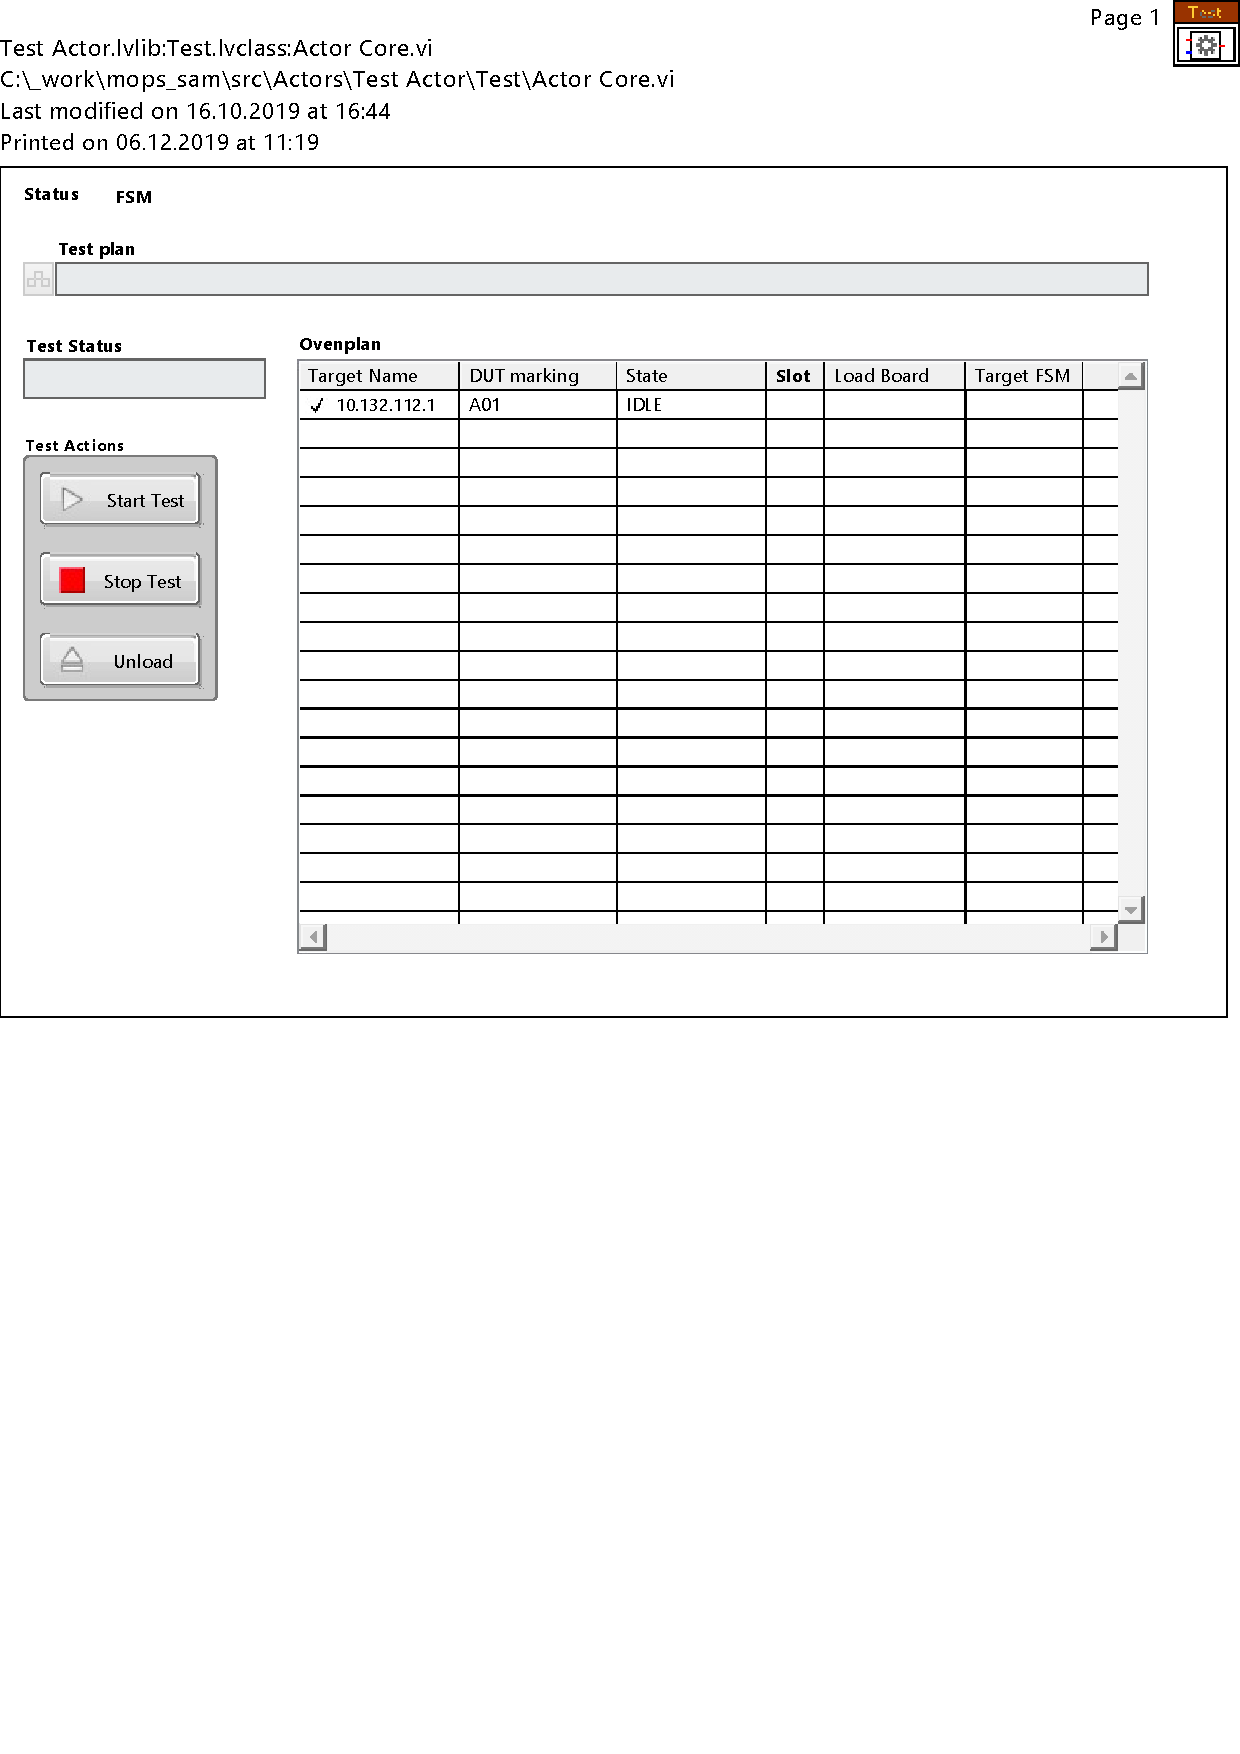
\includegraphics[trim=0 400 0 100, clip, width=100mm]{images/Testactor.pdf}
		\caption{Test Actor}
		\label{fig:Test}
\end{figure}

\item \textbf{Test Actor} Test actor provides a GUI platform to display the test status to the user and also provides the interface to send test events to the control module. 
GUI display of Test Actor is as shown in the \cref{fig:Test}. 
To start the test, "start" is the event that is executed. 
To stop the test, "stop" is the event that is executed. 
Once, when the test starts running, the analog measurements can be acquired by an event "meas", which is executed from the \gls{FSM} window of Test actor. 
Test actor in much general sense executes the finite state machine given in the test plan (see \cref{sec:TP}).    
\end{itemize}

\begin{figure}[hbt]
		\centering
		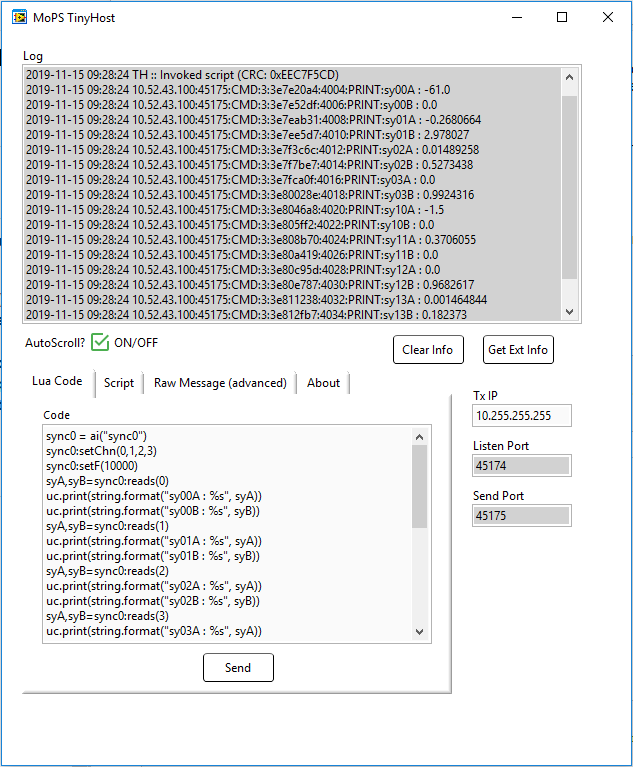
\includegraphics[trim=0 0 0 0, clip, width=100mm, scale=0.75]{images/Tinyhostaichannels.PNG}
		\caption{TinyHost application}
		\label{fig:tinyhost}
\end{figure}


\subsubsection{TinyHost}\label{sec:TinyHost}
A small application called TinyHost exists to test the communication interface of the MicroMoPS and also to send messages to the hardware targets. 
Through, this application the messages can be sent to the hardware targets manually and thereby, commands that are part of Lua interpreter which are present in the microcontroller's firmware are executed. 
To get a sense of TinyHost's purpose, an example of one of the tests that are performed during this thesis is considered. 
In this work, to test the functionality of hardware target's analog input communication modules and their channels' value (see \cref{sec:Channels}), Lua code (see \cref{sec:Lua}) is written to invoke Lua commands that are present at the Lua space of microcontroller's firmware, as shown in the \cref{fig:tinyhost}. 
Subsequently, the result is displayed on the log field of the TinyHost as shown in the \cref{fig:tinyhost}. 
\subsubsection{Test Plan Builder}\label{sec:TP}
Test plan builder~\cite{Plankensteiner2015} is an application used to create a test plan in the form of a \acrshort{FSM} diagram where each state of the FSM diagram is fundamentally a set of Lua commands that are defined in the microcontroller's firmware. 
Test plan builder also downloads the \acrshort{EDS} from the MoPS web server to know the details of the latest hardware configuration of MicroMoPS. Consequently, from the knowledge of hardware configurations, Test-plan builder enables the test engineers to create a test plan. 
The development procedure of test plans and the syntactic rules that are applicable to successfully build test plans are described in detail in Plankensteiner's Master thesis~\cite{Plankensteiner2015}. 
EDS configuration information is necessary for verifying the respective hardware capabilities before a test starts. 
The Test-Plan Builder requires this information to provide knowledge to test design engineers about the available hardware and software modules that could be used in creating test plans. 
A sample of the test plan is as shown in the \cref{fig:Testplan builder}. 
In principle, there are two sections in the layout of a Test plan tab of Test plan builder, they are:  

%Test-Plan builder is the application that downloads the new and updated EDS files from the webserver to validate test plans. 

\begin{figure}[hbt]
		\centering
		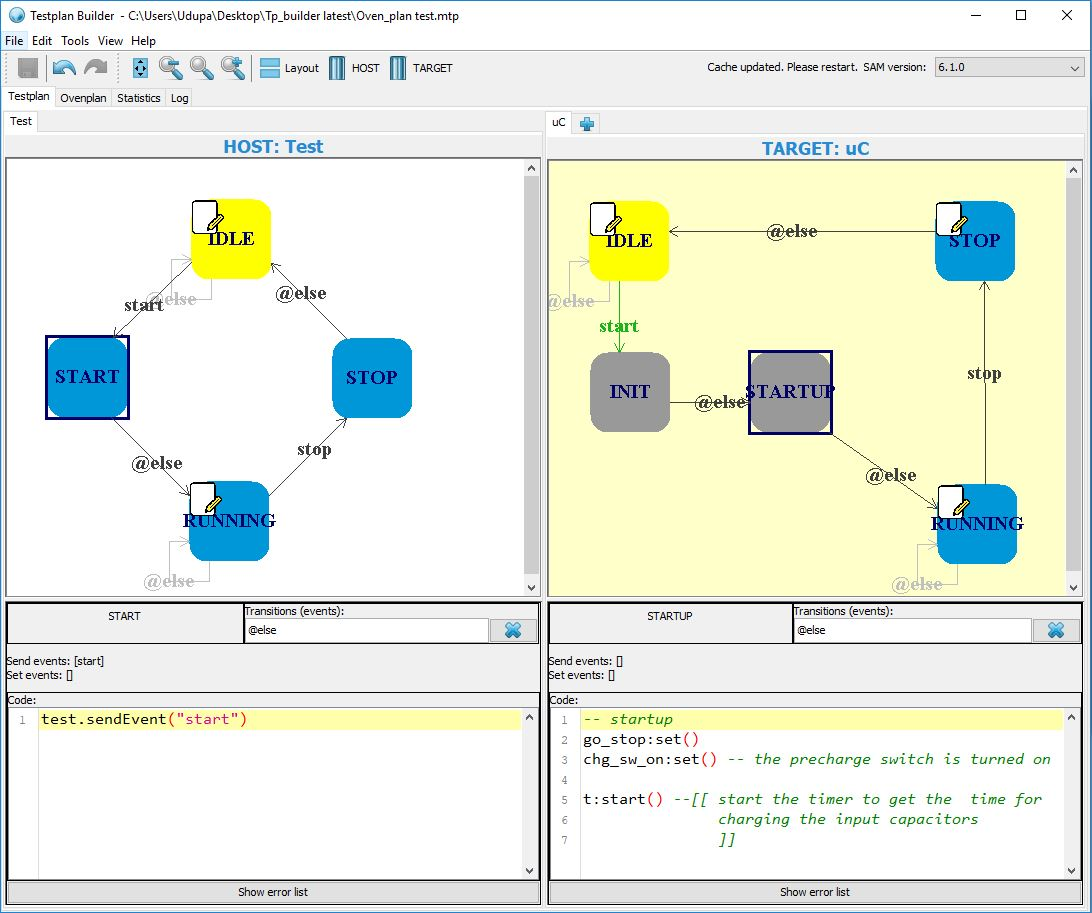
\includegraphics[trim=0 0 0 0, clip, width=150mm]{images/TPbuilder.JPG}
		\caption{Test plan builder application}
		\label{fig:Testplan builder}
\end{figure}

\begin{figure}[hbt]
		\centering
		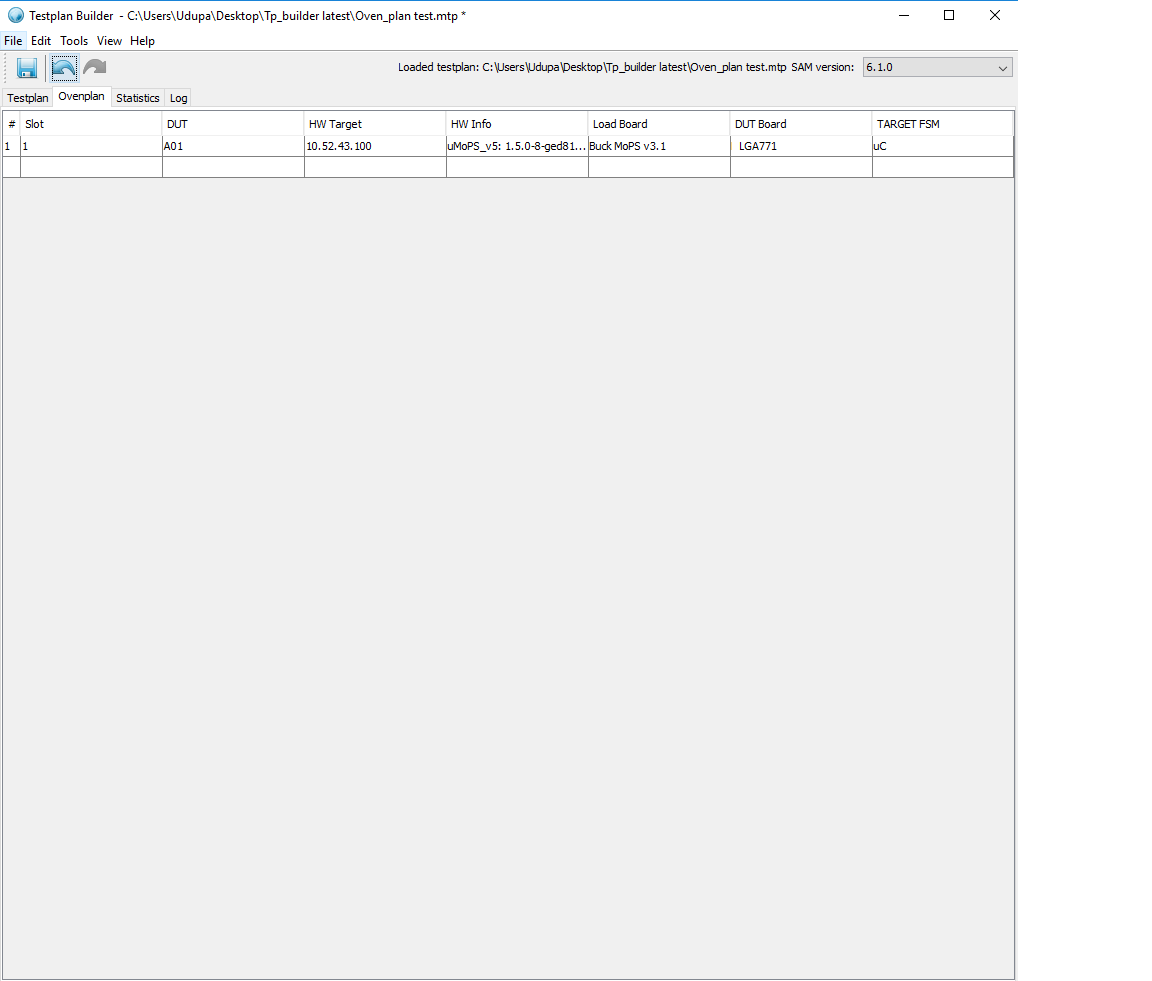
\includegraphics[trim=0 600 0 0, clip, width=\textwidth, scale=0.75]{images/Ovenplan_edited.PNG}
		\caption{Oven plan window}
		\label{sec:Oven plan window}
\end{figure}

\begin{enumerate}
\item \textbf{HOST:} The \acrshort{FSM} diagram in Host is meant for providing control over the operation of the Target FSM diagram. 
As soon as the start button is pressed after loading the test plan to SAM, there occurs a transition from the IDLE state of Host FSM to the START state in test execution. 
This START state machine sends a "start" event to the IDLE state machine of Target FSM which, leads Target FSM to propagate further from the IDLE state.
    
\item \textbf{TARGET:} The FSM diagram in Target is the starting point for the control module to subject \acrshort{DUT} into stress, where the functionality of Target FSM is totally controlled by the Host FSM.
Intuitively, the running of all the state machines of Target FSM except INIT is nothing but the invoking of Lua commands that are specific to microcontroller's firmware modules (\cite{Steinwender2016}, p.39). 
As soon as Target FSM is triggered by Host FSM by receiving a start event, there occurs a transition from the IDLE state to the INIT state in Target FSM. 
Consequently, at INIT a digital stimuli is generated towards the DUT because of the PWM signal from the control module. 
Furthermore, Target FSM reaches to running state which, is an indication that the test is running. 
Finally, the test is stopped by pressing a stop button in SAM, which results in the Target FSM diagram to reach to its IDLE state from any given state.  
\end{enumerate}

%In this work, the more concentration is towards the information that is generated because of the entries that are provided in the oven plan. 
\textbf{Oven plan} The oven plan of the Test plan builder tool provides an interface to select desired DUT, application module and Hardware target. 
Test engineers select the board names based on the stress type they want to perform. 
The selection of boards is done by a drop-down present in the oven plan window of the test plan builder. 
A variant of MicroMoPS (classified by their IP address), Application module and DUT are chosen as shown in the \cref{sec:Oven plan window}.     
The test FSM diagram in the test plan window and hardware selection in the oven plan window fulfills the protocol of the creation of the test plan. 
Further, to which the test plan is generated as a JSON file. 
The JSON file is loaded to SAM to execute the stress test. %In the meantime, SAM uses the same JSON file counterpart to fetch the board names that are selected by test engineers.

%In addition to the fundamental modules that drive microcontroller firmware, another handler is developed such as test\_identify\_boards() to reach one of the milestones of this thesis.


%To consider explaination in terms of ADC conversion by referring Versatile Analog to Digital Converter.
\subsection{Measurement environment of MoPS}\label{sec:ME}

This section describes the measurement data acquisition system of MicroMoPS, measurements communicating channels of MicroMoPS, signal conditioning circuits present in the measurement environment and processing concepts. 

\subsubsection{Measurement data acquisition of MicroMoPS}\label{sec:DAQ} 
\glsentryfull{DAQ} of MicroMoPS is responsible for acquiring, displaying and storing the analog measurements that are obtained from tests. 
The analog measurements such as temperature, voltage, and current of the test are sent to Analog-to-digital converter (ADC) of the MicroMoPS via dedicated analog input channels. 
These measurements that are received at the ADC of MicroMoPS, are sampled and quantized to convert into a certain range of digital values. 
In general, the ADC of a MicroMoPS is of 12 bit resolution, therefore the analog values that are converted into digital values range from 0 and 4095 and represent the microcontroller's specific voltage values range from \SIrange{0}{3}{\volt}. 
These measurements go through some signal conditioning (see \cref{fig:Conditioning}) before they are used by the ADC to perform digital conversion.
The analog measurements that are communicated using analog communication channels are classified into two types: 
\begin{enumerate}
\item \textbf{Single-ended multi-channel measurements:} This type of measurement requires the analog value to be referenced to the well chosen common-mode i.e. Ground.
\item \textbf{Differential measurements:} This type of measurement does not have common-mode reference but have a difference in analog value between the two input signal leads.
\end{enumerate}

The communication channels which conduct analog measurements follow a certain hierarchy in their design (see \cref{Channels}) and these measurements are converted from differential measurements/single-ended channel measurements to single-ended values by allowing them to go through signal conditioning. 
Because of this, the measurements are achieved in delimiting them into the microcontroller operating voltage range i.e., \SIrange{0}{3.3}{\volt}.

\subsubsection{Channels hierarchy and their purpose}\label{sec:Channels}
Analog-to-digital conversions in MicroMoPS can be executed in two modes. They are:
\begin{enumerate}
\item \textbf{Synchronous mode} - Channels belonging to a synchronous group can do an analog-to-digital conversion in parallel as the ADC kernels of these channels are synchronized with each other.  
\item \textbf{Scan mode} - Channels belonging to the scan group follow a configurable linear sequence that allows the dedicated channels to do analog-to-digital conversion one after another.
\end{enumerate}
\begin{figure}[hbt]
		\centering
		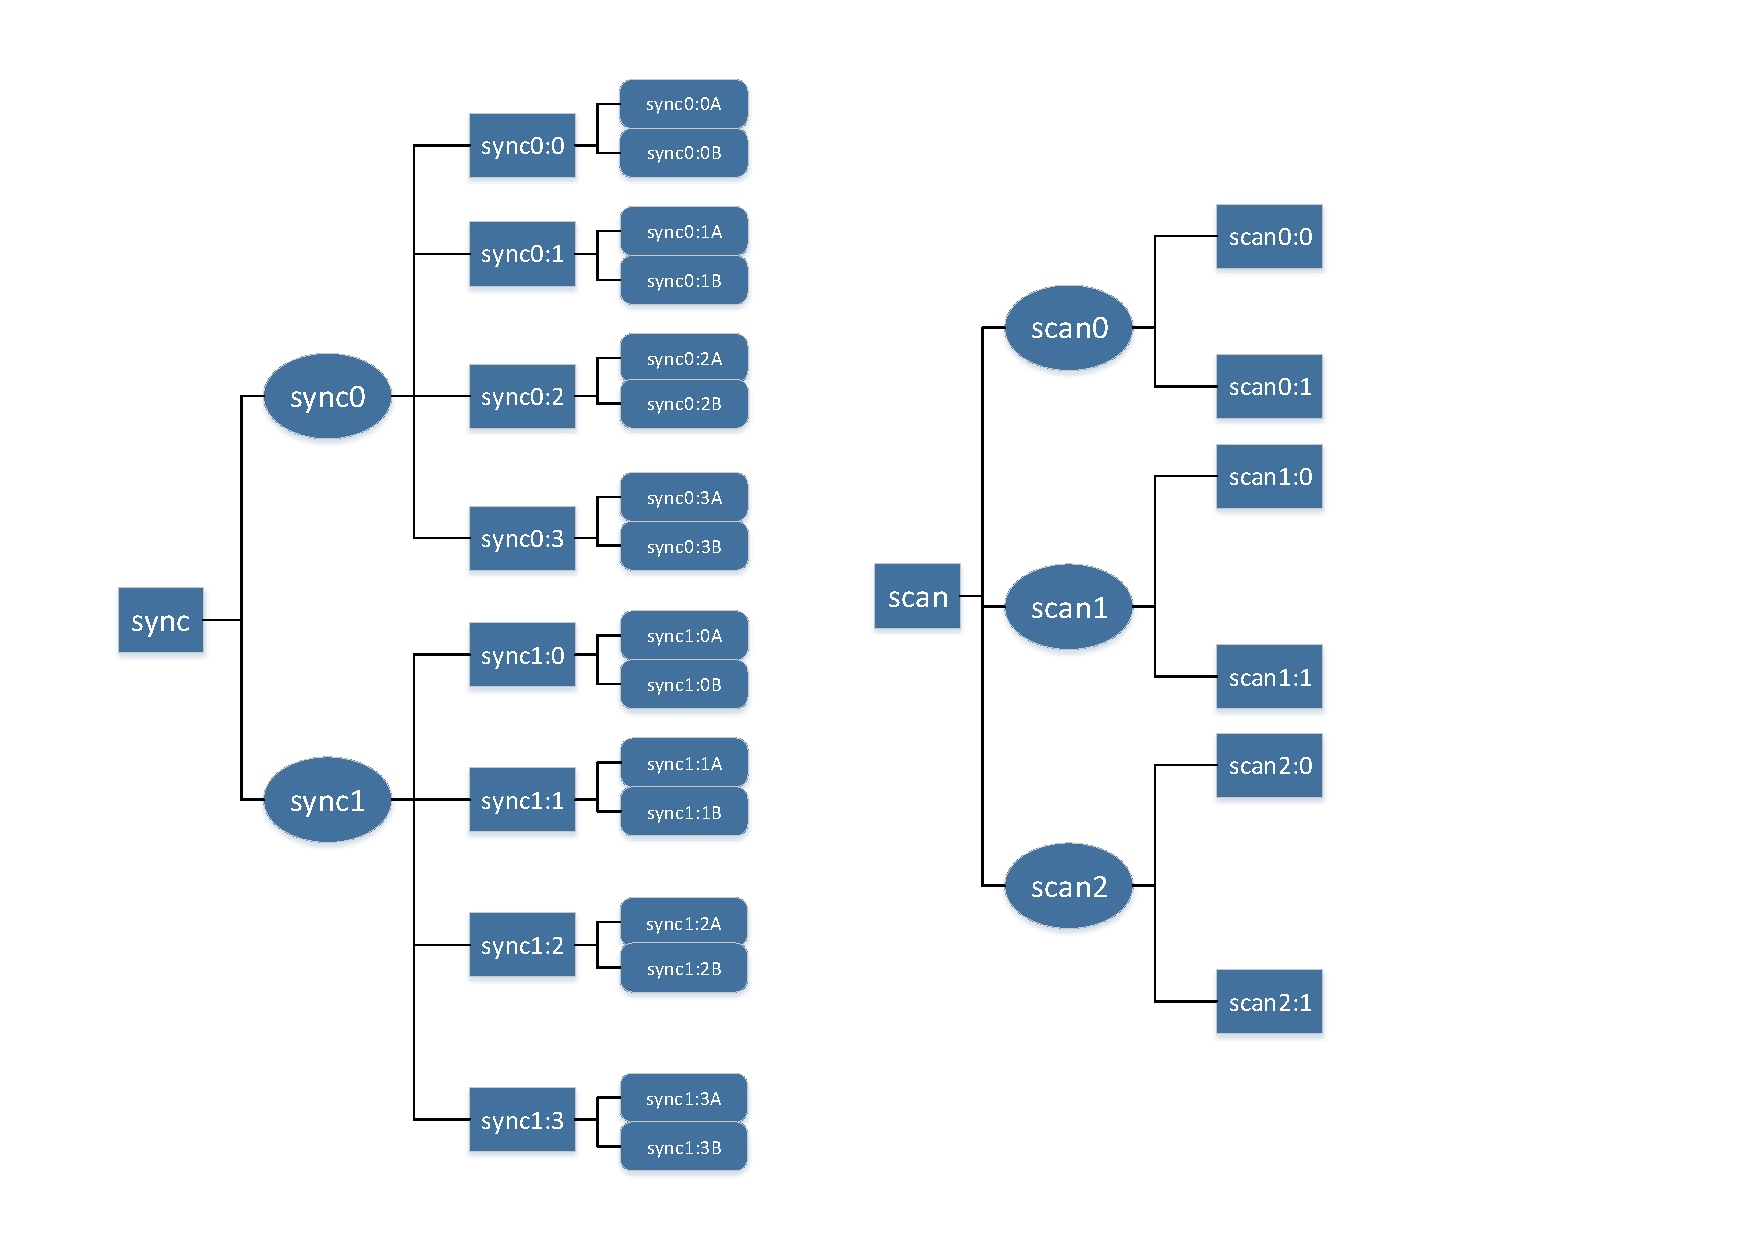
\includegraphics[trim=0 0 50 0, clip, width=125mm, scale=0.75]{images/channels_hierarchy.pdf}
		\caption{Channels hierarchy}
		\label{Channels}
\end{figure}
With respect to the modes of analog-to-digital conversion, there are dedicated channel modules such as sync0, sync1, scan0, scan1, and scan2. The mentioned channel modules as they are named, correspond to synchronous and scan conversion modes. These channel modules are further classified as follows:
\begin{enumerate}
\item \textbf{sync[0,1][0,3]B} - Unipolar Analog-to-Digital conversion synchronous channels, where first index, i.e, [0,1] represents the module number, second index, i.e, [0,3] represents the module's specific channel number and third index represents the channel's specific group name. 
The group name assigned to this channel is 'B'.    
\item \textbf{sync[0,1][0,3]A[N,P]} - Bipolar Analog-to-Digital conversion synchronous channels, where first index, i.e, [0,1] represents the module number, second index, i.e, [0,3] represents the module's specific channel number and third index represents the channel's specific group together with the polarity, i.e, -/+ of the elelctrical signal. The group name assigned to this channel is 'A'.
\item \textbf{scan[0,1,2][0,1]} - Analog-to-Digital conversion scan channels, where first index, i.e, [0,1] represents the module number, second index, i.e, [0,1] represents the module's specific channel number.
\end{enumerate}

The Differential Voltage measurements such as Switch Node Voltage (Vswh),  Measurement voltage from Auxiliary MicroMoPS node 1 (Aux1), IC current monitor (Imon), Converter input voltage (Vin) and Converter output voltage (Vout) are acquired via bipolar Analog-to-Digital conversion channels i.e. \textbf{sync[0,1][0,3]A[N,P]}.
Aux1 and Aux2 are the auxiliary MicroMoPS that are used to cover multiple functions available on the test device.

The single ended Voltage or Current or Temperature measurements such as Converter input current (Iin), Converter output current (Iout), DUT case temperature (Tc), DUT board temperature (Tbrd), Driver current (Idrv), Driver Voltage (Vdrv), IC current monitor (Imon) and IC temperature monitor (Tmon) are acquired via unipolar analog-to-digital conversion synchronous channels i.e. \textbf{sync[0,1][0,3]B}. 

The above measurement parameters are part of the Low Voltage MTS environment~\cite{Sleik2018a}.

\subsubsection{Analog signal conditioning circuits}\label{sec:asc}
To most of the measurement signals, the analog signal conditioning circuit setting is merely the differential amplifier with a series resistor and standard voltage divider circuits convention as shown in the \cref{fig:Conditioning}. This signal conditioning circuit is designed by the hardware designers of KAI.  
\begin{figure}[htb]
		\centering
		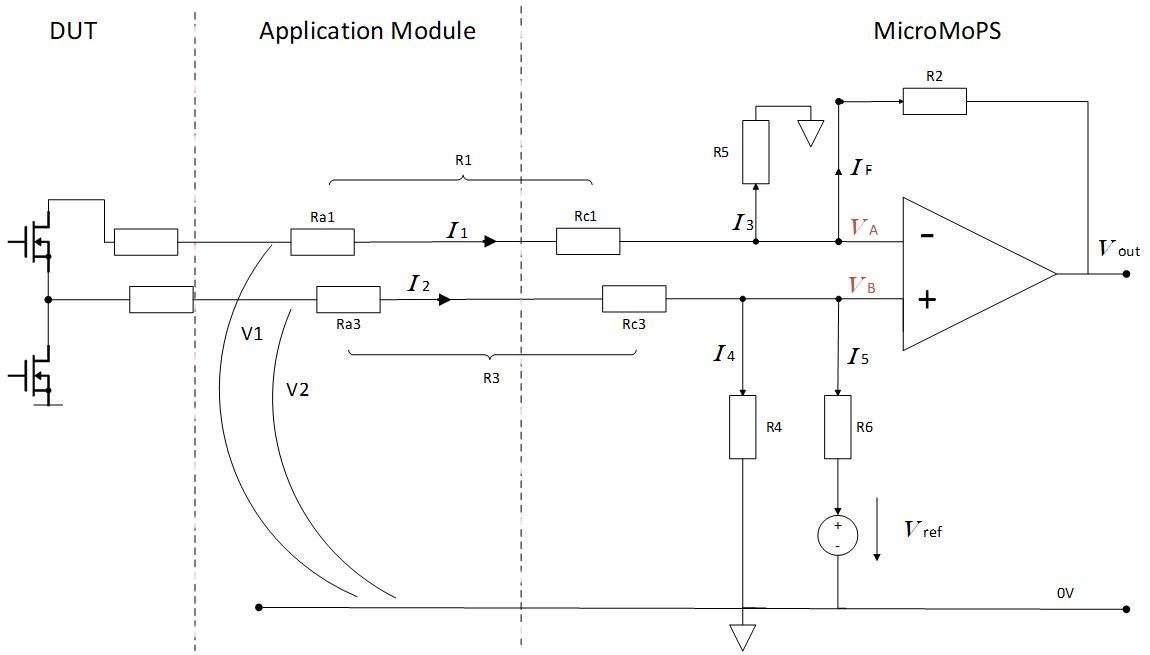
\includegraphics[trim=10 0 0 0, clip, width=150mm, scale=0.75]{images/conditioning.JPG}
		\caption{Analog signal conditioning circuit}
		\label{fig:Conditioning}
\end{figure}

Conditioning of the voltage, temperature, and current signals is achieved by using an analog signal conditioning circuit (see \cref{fig:Conditioning}) with some standard component values. 
The analog signal conditioning circuit for \gls{Iin} and \gls{Iout} are placed on the application module and the resulting conditioned signal is directly fed to analog-to-digital converters of the control module. 
The analog signal conditioning circuit for \gls{Vin}, \gls{Vout} and \gls{Imon} are placed on the control module. 
For the DUT case temperature measurement i.e. \gls{Tcase}, the resistive sensor is supplied from a constant current source with a provision of voltage amplification. \gls{Tmon} in an application module to monitor the DUT temperature. 
\gls{Vdrv} in the application module consists of a Voltage divider circuit to drive MicroMoPS. 
Finally, \gls{Idrv} in the application module to supply current to MicroMoPS.

\subsubsection{Processing concepts}\label{sec:Pc}
Finally, in order to convert the digital measurements (representative of the analog measurements of the \acrshort{DUT}) into microcontroller's specific analog values which range from \SIrange{0}{3}{\volt}, the respective digital values need to be processed.
The method of processing digital values is called a scaling function. This scaling function can vary from channel to channel because of the varying microcontroller specific analog value range for particular test measurements. 
For an instance, the microcontroller specific analog value range for the channel \textbf{sync[1][0]A} ranges from \SIrange{-1.5}{+1.5}{\volt} whereas, the microcontroller specific analog value bandwidth for the channel \textbf{sync[0][0]B} ranges from \SIrange{0}{3}{\volt}. 
Standard scaling function (see \cref{eq:Scaling}) is used to process the analog measurements.  

\section{State of the art}\label{sec:SOA}
Stress test application on a high level goes at a particular flow. 
This flow essentially provides the state of the art that exists in this stress test environment.
The flow of the stress test as depicted in \cref{fig:SOA} is explained accordingly in steps as follows:   

\begin{figure}[htb]
		\centering
		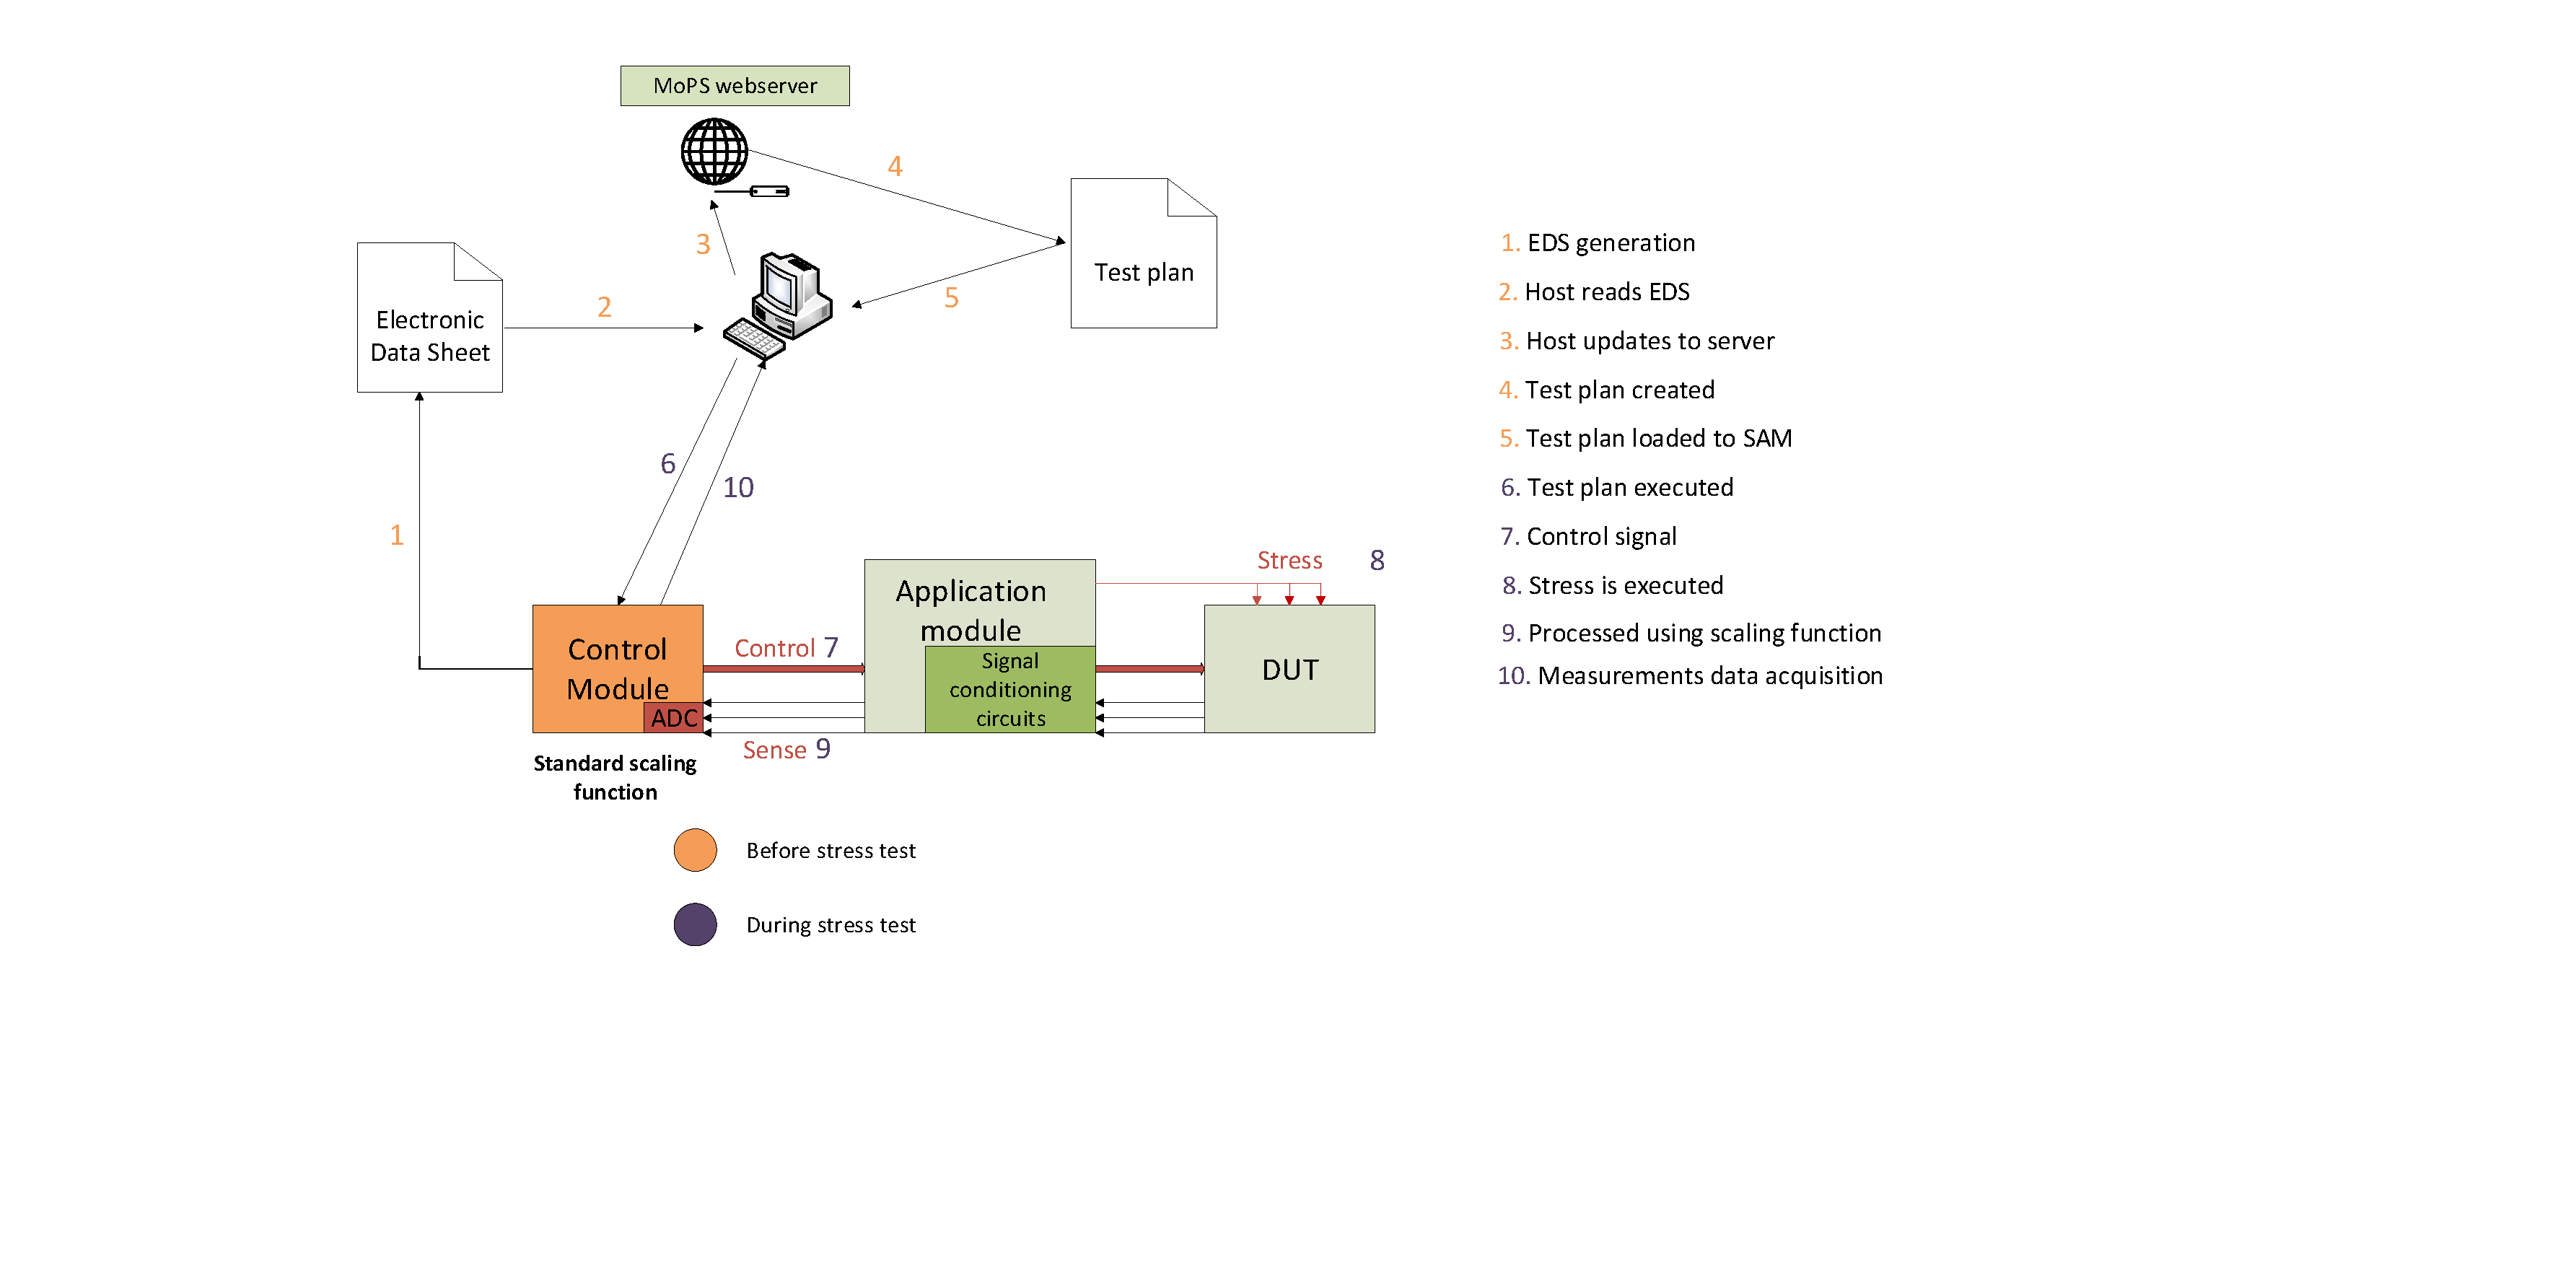
\includegraphics[trim=150 300 750 0, clip, width=\textwidth, scale=0.75]{images/Software_architecture.pdf}
		\caption{State of the art}
		\label{fig:SOA}
\end{figure}

\begin{enumerate}
\item The starting point of the stress test application is from the control module. A control module is flashed with a stress test application integrated firmware image to execute the test plan. Upon booting of microcontroller, an \acrshort{EDS} is generated in the MoPS CORE firmware project folder.
\item SAM accesses the latest \acrshort{EDS} that is generated in the MoPS CORE firmware project folder.
\item SAM further updates the latest EDS to MoPS web server.
\item Test plan builder tool downloads the EDS to create and validate the test plans that are created by test engineers.
\item A Semiconductor is not subjected to stress test until this point. SAM further keeps waiting to receive test plans to subject DUT into an application-specific stress test.
 Subsequently, Test plans (see \cref{sec:TP}) that are created by test engineers are loaded to SAM.
\item Test plans are forwarded by SAM to MicroMoPS for it's execution.
\item Test plans are executed and as a part of execution, the PWM signal is sent from the control Module to \acrshort{DUT}. 
The control (PWM) signal makes the DUT go into an operational mode.
\item Electrical stresses are applied onto DUT through the application module.
\item Electrical signals are generated in the DUT because of the electrical stresses that are exerted on the semiconductor device.
\item The generated electrical signals are measured through the analog communication channels of MicroMoPS.
\item The analog measurements are digitized using an ADC of MicroMoPS and the digitized values are later processed using a standard scaling function (see \cref{sec:ADC}) to convert them into discrete MicroMoPS specific voltage values.
\item The processed data are acquired by SAM to retain the original values of analog measurements. The retained values are used in the SAM for further interpretation such as, for calculating the end of life of DUT. 
\end{enumerate}     

\afterpage{\null\newpage}
\afterpage{\null\newpage}
%\cleardoubleplainpage
%\cleardoubleplainpage
\chapter{Approach and Methodology}
\section{Overview}
After understanding the scope of improvement in the existing analog measurement signals processing methodology,
a new approach is worked out and implemented within the Low Voltage MTS setup.
The new approach involves some action items that are needed to be completed at a certain chronology.
The sequence of action items is depicted in \cref{fig:flowchart}.
\Cref{sec:dataproc} describes the data processing concepts that are derived for processing analog measurements in MicroMoPS. 
\Cref{sec:identification} describes the identification of boards in the stress test environment and preparation of board related information in the MoPS web server.
\Cref{sec:host application} describes the automated procedure of processing analog measurements regardless of the board combinations.
\begin{figure}[hbt]
		\centering
		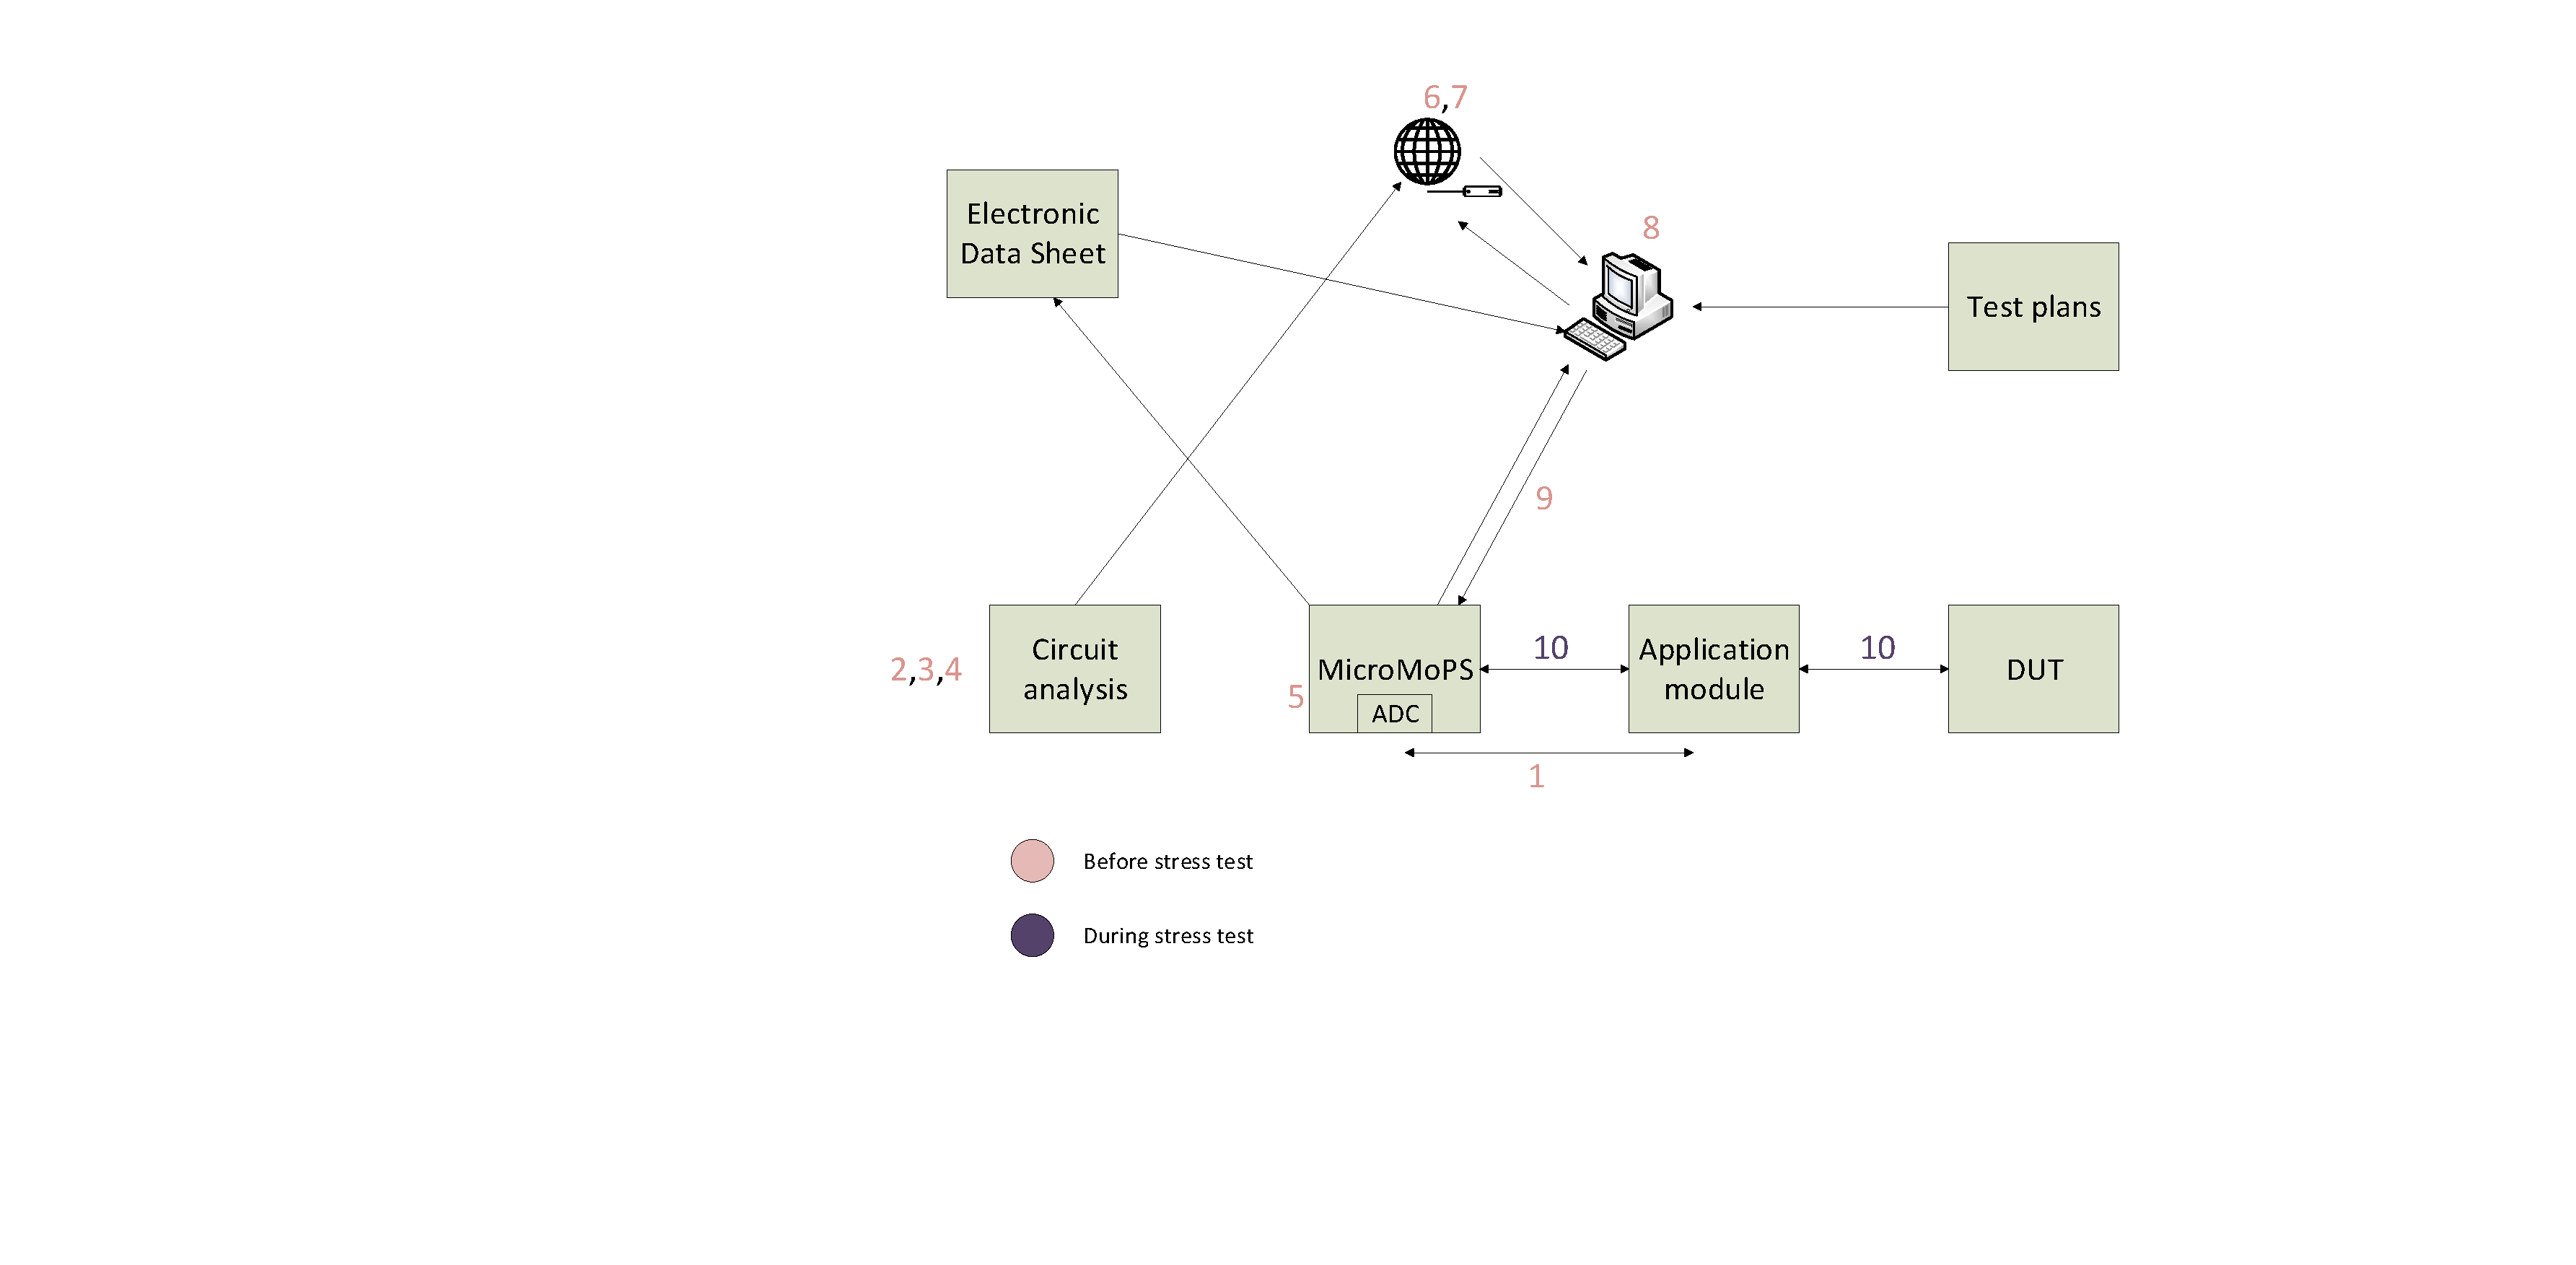
\includegraphics[trim=540 150 0 0, clip, width=195mm]{images/Approach_and_methodology.pdf}
		\caption{Enhancements.}
		\label{fig:flowchart}
\end{figure} 

\section{Derive data processing concepts for stress test environment}\label{sec:dataproc}

\subsection{Acquiring a signal model}\label{sec:SM}	
	\begin{figure}
	\centering
	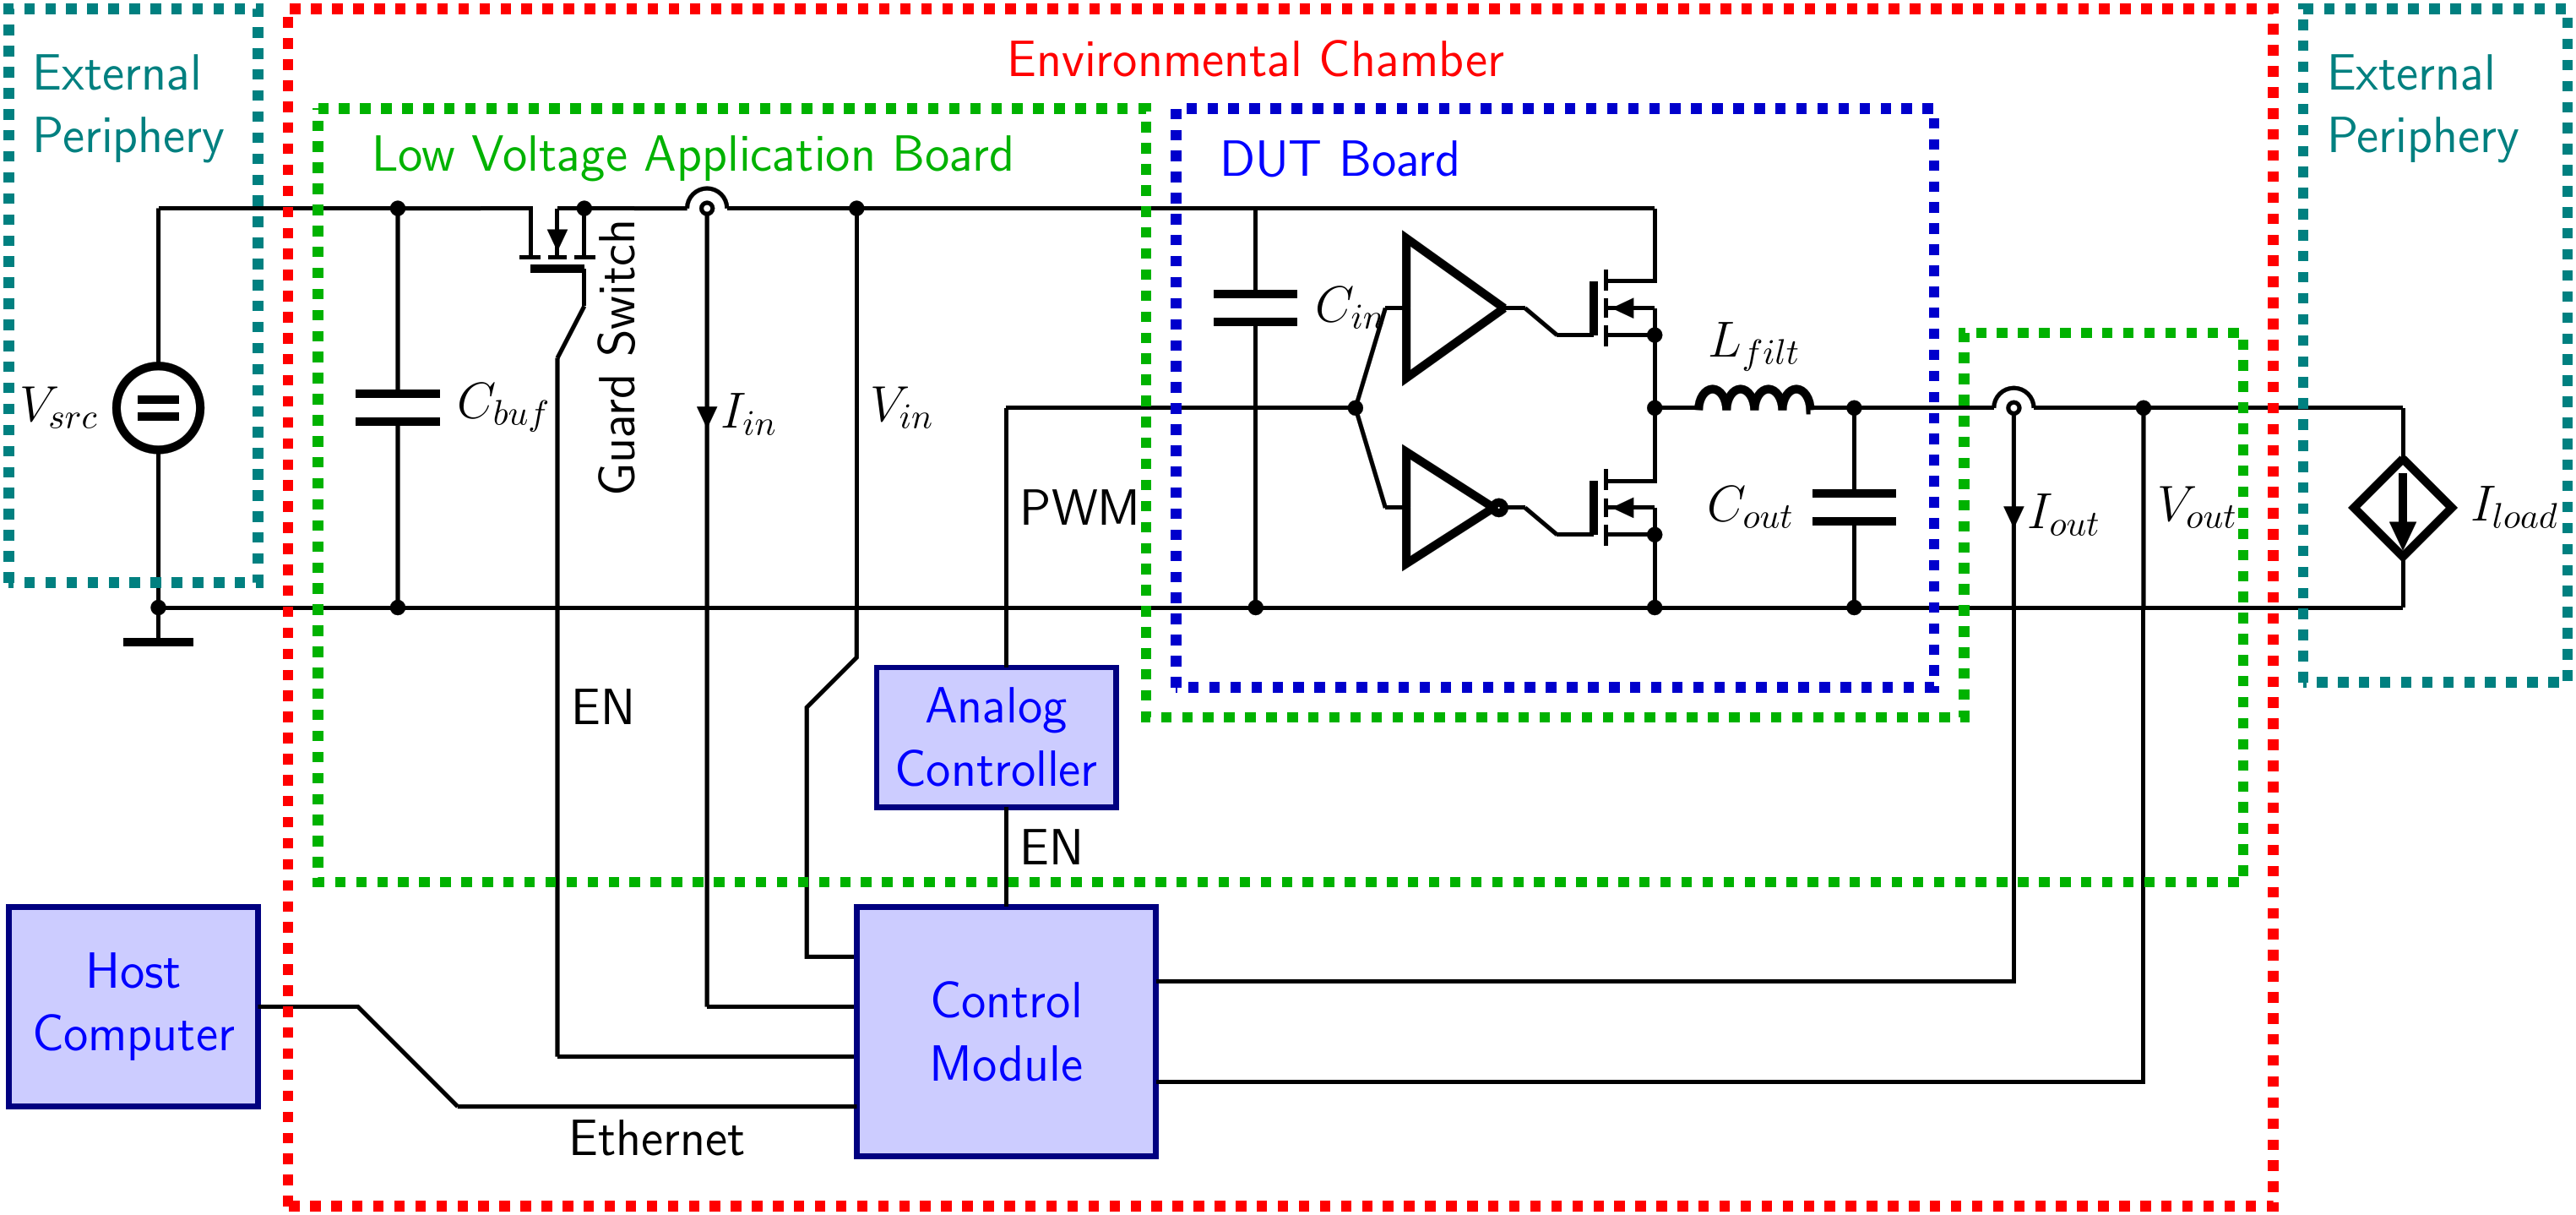
\includegraphics[trim=0 0 0 0, clip, width=\textwidth]{images/LV_module_2.png}
	\caption{Low Voltage Modular test system.}
	\label{fig:LVMTS}
	\end{figure}

In the modular stress test environment, the application module is used for submitting stresses on DUT. 
The used application module involves its own application specific characteristic circuitry.
In this work, since it is the Low-Voltage stress test system that is used, the discrete power transistors are submitted to \emph{power cycling} (~\cite{Sleik2016}, p.2) test. 
This is a test in which \acrshort{DUT}s are pulled to their extreme operating conditions by introducing them into various scenarios. %DUTs are heated to reach temperature between \SIlist{85;125}{\celsius} for consumer devices, \SI{150}{\celsius} for automotive devices and are supplied with supply voltage that is set to maximum level which still complies the data sheet specificiation of DUT. Intermittent loads are submitted to DUTs which toggle between a high load of \SI{100}{\percent} that nearly reaching DUTs to their maximum operating temperature and a low load of \SI{10}{\percent}.} 
Further, in response to a "power cycling" test, certain \acrshort{MTS} parameters are measured. %such as Iin, Iout, Vin, Vout, Tcase, Idrv, Vdrv, Imon and Tmon(see Section \cref{Channels}).
These parameters of the Low Voltage MTS are recorded based on the control logic implemented by a PI controller at BuckMoPS (\cref{sec:BuckMoPS}). 
As a result, the measurement signals are automatically monitored by a control module throughout the entire test. 
These measurement signals go through conditioning before reaching the ADC, as explained in \cref{sec:asc}. 
To obtain the real time efficient scaling mechanism for MicroMoPS, the path that the measurement signals traverse from the source of the signal conditioning circuits to the source of the analog-to-digital converter of the control module as shown in \cref{fig:Signal model}, are analysed in this work. 
The path that the measurement signals travel consist of the measurement circuits that are associated with acquisition of measurements. 
Further, the signal path information is obtained by following the hardware schematics of MicroMoPS and application module. 
The values of every active and passive device that are present in the measurement circuitry is important to know because it helps in obtaining scaling factor associated parameters which are specific to the respective type of measurements.
\begin{figure}[htb]
	\centering
	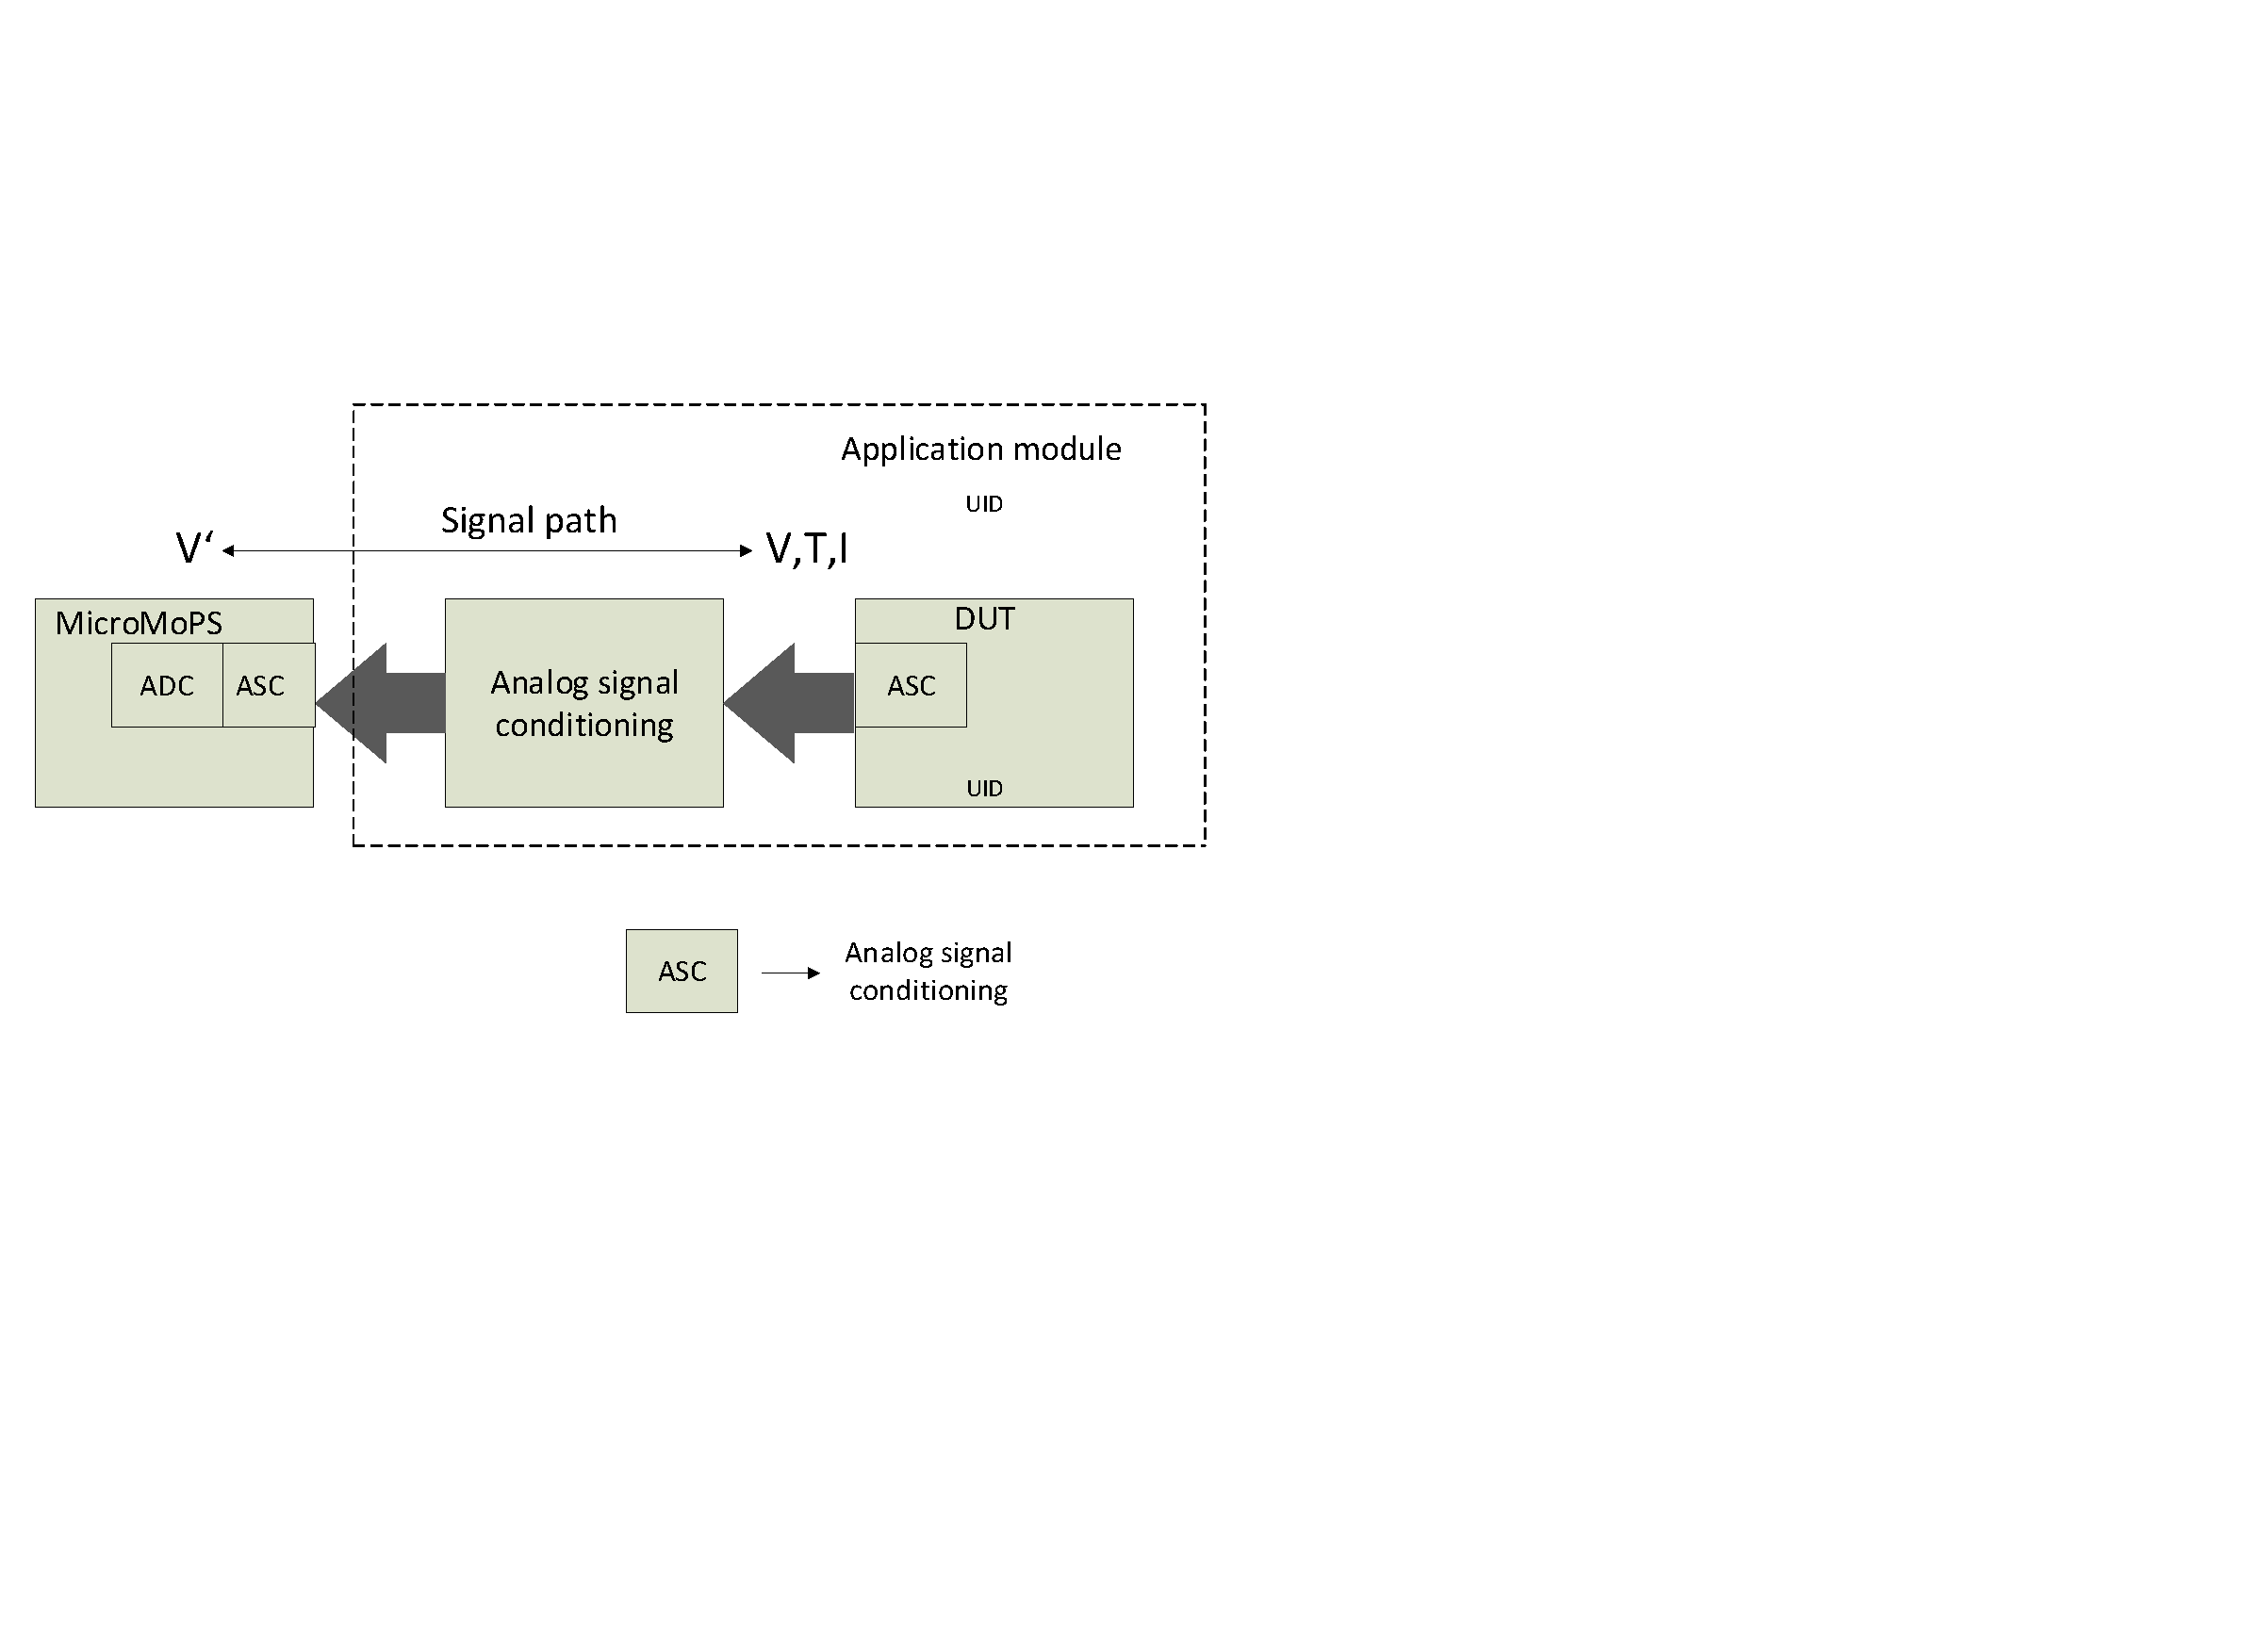
\includegraphics[trim=0 400 400 150, clip, width=\textwidth]{images/Signalmodel.pdf}
	\caption{Signal path of measurement data acquisition.}
	\label{fig:Signal model}
\end{figure}

The series resistors (R1, R3), differential operational amplifier and the standard voltage divider circuit (R2, R4, R5 and R6) conventions (see \cref{fig:Conditioning}) are part of the analog signal conditioning circuit as described in \cref{sec:asc}. 
They are defined by Hardware designers at KAI to appropriately attenuate the electrical signals into MicroMoPS operating voltage range from \SIrange{0}{3}{\volt}.
The defined circuit component values are listed as shown in \cref{Table1}.

%Assumptions of circuit components
%\vspace{2cm}
%\centering

\begin{table}
	\centering
	\caption{Component values}
	\label{Table1}
	\begin{tabular}{ |p{3cm}||p{1.5cm}|p{1.5cm}|p{1.2cm}|p{1cm}|p{1.2cm}|p{1cm}|  }
	\hline
	\textbf{Signal}   & \textbf{R1}    &\textbf{R2}   &\textbf{R3}   &\textbf{R4}   &\textbf{R5}   &\textbf{R6}\\
	\hline
	Iin   &\SI{18}{\kilo\ohm}   &60k\si{\ohm}   &18k\si{\ohm}   &60k\si{\ohm}   &15k\si{\ohm}   &15k\si{\ohm}\\
	Iout   &27k\si{\ohm}    &60k\si{\ohm}   &27k\si{\ohm}   &60k\si{\ohm}   &75k\si{\ohm}   &75k\si{\ohm}\\
	Vin   &26.9k\si{\ohm}    &4.02K\si{\ohm}   &26.9k\si{\ohm}   &2k\si{\ohm}   &NP   &NP\\
	Vout   &6.7k\si{\ohm}    &4.02K\si{\ohm}   &6.7k\si{\ohm}   &2k\si{\ohm}   &NP   &NP\\  	
	Imon   &2k\si{\ohm}    &2k\si{\ohm}   &2k\si{\ohm}   &2k\si{\ohm}   &4.02k\si{\ohm}   &2k\si{\ohm}\\
	\hline
	\end{tabular}
	\label{table:circuit_components}
\end{table}

		\subsection{Derive transfer characteristics to find scaling parameters.}\label{sec:Transfer Function}
		After obtaining a signal model which provides information about the measurement circuit of the Low Voltage stress test environment, the circuits that are present in the signal path are analysed to derive the transfer function between the source of the signal conditioning circuits and the source of the analog-to-digital converter of the MicroMoPS. 
		Derivation of the transfer function is done using one of the standard circuit analysis techniques (e.g. Superposition theorem).  
Measurements such as \gls{Vin}, \gls{Vout}, \gls{Iin}, \gls{Imon} and \gls{Iout} with differential amplifier circuits (see \cref{sec:asc}) are analysed using Superposition theorem. 
Using the Superposition theorem, three equations of input/output relations are obtained from which, the transfer function is derived. 
The derived transfer function is further simplified. The steps that are involved in deriving the transfer function are as follows: 
%Transfer function steps and simplification

\begin{enumerate}
  \centering
\item $V_1$ and $V_2$ are shorted.\\
	\vspace{4mm}
	\hspace{30mm}
	  %$V_01$ = $V_ref$.\[ \cfrac{V_ref}{b} \] 
	  	$V_{o1}$ = $V_{ref}$ .$\dfrac{R_3||R_4}{R_6 + R_3||R_4}$.$\left(1 + \dfrac{R_2}{R_1 + R_5}\right)$
\item $V_1$ and $V_{ref}$ are shorted.\\
	\vspace{4mm}
	\hspace{28mm}
	  %$V_01$ = $V_ref$.\[ \cfrac{V_ref}{b} \] 
	  $V_{o2}$ = $V_{2}$ .$\dfrac{R_4||R_6}{R_3 + R_4||R_6}$.$\left(1 + \dfrac{R_2}{R_1 + R_5}\right)$
\item $V_2$ and $V_{ref}$ are shorted.\\
	\vspace{4mm}
	\hspace{-9mm}
	  %$V_01$ = $V_ref$.\[ \cfrac{V_ref}{b} \] 
	  $V_{o3}$ = $V_{1}$ .$\left(-\dfrac{R_2}{R_1}\right)$
\end{enumerate}

\begin{flushleft}
\hspace{-9mm}
$V_{out}$ results in $V_{out}$ = $V_{o1}$ + $V_{o2}$ + $V_{o3}$, which equals the expression of nodal analysis, i.e.

\hspace{-9mm}
$V_{out}$ = $\dfrac{R_3R_4R_6}{R_3R_4 + R_3R_6 + R_4R_6}$$\left(\dfrac{R_2}{R_1 + R_5} + \dfrac{V_{ref}}{R_6}\right)$$\left(1 + \dfrac{R_2}{R_1} + \dfrac{R_2}{R_5}\right)$ - $\dfrac{R_2}{R_1}V_1$.

\hspace{-9mm}
The resistor relations assumptions are applied:


\hspace{-9mm}
${R_1}$ = ${R_3}$\\
\hspace{-9mm}
${R_2}$ = ${R_4}$\\
\hspace{-9mm}
${R_5}$ = ${R_6}$

\hspace{-9mm}
This further simplifies the $V_{out}$ equation to

\hspace{-9mm}
$V_{out}$ = $\dfrac{R_2}{R_1}$($V_{1}$ - $V_{2}$) + $\dfrac{R_2}{R_5}$$V_{ref}$, \hspace{9mm} where ($V_{1}$ - $V_{2}$) = $V_{in}$ 
\end{flushleft}

\hspace{-10mm}Further, the information of MicroMoPS' voltage range and resistor values as described in \cref{sec:Channels} and \cref{table:circuit_components}, respectively, are specific to measurement channels. These values are plugged into the derived transfer function to 
obtain the measurement range of the voltage or current or temperature signal before 
conditioning. The algebraic method of performing the above explained calculation is 
demonstrated by considering a '\acrshort{Vin}' measurement parameter's signal path as an example.	

\hspace{-10mm}
For '$V_{in}$' measurement parameter the $V_{out}$ equation simplifies to,
%algebraic expression using example

\begin{equation}
V_{out} = \dfrac{R_2}{R_1}.V_{in}, 
\label{eq:Vout}
\end{equation}

\hspace{-10mm}
To find '$V_{in}$' measurement range, the maximum voltage condition of MicroMoPS is considered and the values corresponding to $V_{in}$ are put to \cref{eq:Vout},

\hspace{-9mm}3V = $\dfrac{4.02\kilo}{26.9\kilo}V_{imax}$,\\

\hspace{-9mm}-> $V_{imax}$ = 20.17500 V

\hspace{-9mm}Similarly, minimum voltage condition corresponding to $V_{in}$ becomes,

\hspace{-9mm}0V = $\dfrac{4.02\kilo}{26.9\kilo}V_{imin}$, \\

\hspace{-9mm}-> $V_{imin}$ = 0 V

\hspace{-9mm}Likewise, the measurement range of the signal at source is found for all the measurement parameters. They are listed in \cref{Table2}.
%table

\begin{table}[ht]
	\centering
	\caption{Measurements range}
	\label{Table2}
	\begin{tabular}{ |p{3cm}||p{1.5cm}|p{1.5cm}| }
	\hline
	\textbf{Signals}   & \textbf{min}    &\textbf{max} \\
	Iin   &-5A   &10A \\
	Iout   &-5A    &70A\\
	Vin   &0V    &20.175V\\
	Vout   &0V    &5.020V\\  	
	Imon   &0V   &0.305V\\
	\hline
	\end{tabular}
\end{table}

\hspace{-9mm}Also, the measurement range of other parameters are found by either simple nodal analysis method or they are present in hardware schematics of application module. 

\hspace{-9mm}Using the obtained measurement ranges, the measurement specific linear equation fitting scaling parameters are found out. 
The algebraic method of finding out scaling parameters is explained by reconsidering the same measurement parameter, i.e., \acrshort{Vin}. 
%algebraic expresion

\hspace{-9mm}Linear scaling function is given by \\ 
y = k*x + d,      \\
\hspace{9mm} where, y = analog value, \\
\hspace{9mm} k = scaling factor, \\
\hspace{9mm} x = digital representation of analog measurement, \\
\hspace{9mm} d = offset

\hspace{-9mm}For maximum voltage condition of Vin, the digital value is 4095	 (12 bit resolution, see \cref{sec:DAQ}), the analog value is the maximum \acrshort{Vin} measurement from the \cref{Table2}\\

\begin{equation}
20.175 = k(4095) + d
\label{eq:Vmax}
\end{equation}

%\hspace{-9mm}-> 20.175 = k(4095) + d ............(3)

\hspace{-9mm}Similarly, for minimum voltage condition of Vin, the digital value is 0, the analog value is the minimum \acrshort{Vin} measurement from the \cref{Table2}

\begin{equation}
0 = k(0) + d
\label{eq:Vmin}
\end{equation}

%\hspace{-9mm}-> 0 = k(0) + d ............(4)

\hspace{-5mm}Solving \cref{eq:Vmax} and \cref{eq:Vmin} using substitution method, the values of scaling parameters that are associated to \acrshort{Vin} measurement parameter are obtained as below.\\

\hspace{-3.5mm}k = 0.0049267399267399,\\
\hspace{3mm}d = 0

From the obtained scaling parameters 'k' and 'd', it is evident that the found scaling parameters could be used for processing the digitized stress measurements to original signal value (signal before conditioning) but not to MicroMoPS specific voltage range. 
Therefore, the linear equation is further improved by considering additional parameters in the scaling function.   

\subsection{Find a linear scaling function from obtained scaling parameters.}\label{sec:linear function}
The improvement of the linear scaling function as discussed in the previous section is achieved by considering the changing factor inside the linear scaling function. 
The mentioned changing factor influences in determining the appropriate scaling values that precisely process analog measurements into MicroMoPS specific voltage values. It is given by,

%$V_01$ = $V_ref$.\[ \cfrac{V_ref}{b} \]

%y = \[
%		\left[{$\left(k - \dfrac{V_{max}-V'_{max}}{4096}\right)$*x + d}\right]$  V\\ 
%	  \]

\[ y =  
 \left[\left(k - \frac{V_{max}-V'_{max}} {4096}\right)*x + d \right] V
\] 

If the measurement parameter is temperature or voltage signal then, the improved linear scaling equation is as shown below,

%y = $\left[k - \dfrac{(I|T)_{max}*g-V'_{max}}{4096}\right]$*x + d \ldots V\\ 

\[ y = 
 \left[\left(k - \frac{(I|T)_{max}*g-V'_{max}} {4096}\right)*x + d \right] V
\] 

where, 'I' is the current measurement signal and 'T' is the temperature measurement signal.
%equation
	The changing factor represents the change in maximum value of the original (V/T/I) signal and the maximum voltage of the attenuated signal (V') as represented in the \cref{fig:Signal model}. 
	The value '4096' in the equation represents the factor that contributes in the occurring change. 
	Finally, the transconductance parameter 'g' does the necessary conversion of temperature or current signals into respective voltage values (V').

For the measurement parameter \gls{Tcase}~\cite{Sleik2018a}, since it is the resistive sensor that is fed directly on to ADC of the MicroMoPS instead of a differential amplifier, the scaling parameters for $T_{case}$ are found in a differently instead of deriving transfer function.
The DUT board is let to go into temperature ranging between \SIlist{-55;37}{\celsius}.
Consequently, the corresponding voltage that is generated because of voltage amplification for every different board temperature is measured. 
Using the generated voltage information, scaling parameters ('k', 'd') and transconductance parameter ('g') are found. 
Scaling parameters of all the measurements and the measurements respective units are listed in Table 4.3.

\begin{table}[ht]
	\centering
	\label{table:Table3}
	\caption{Measurement parameters}
\begin{tabular}{ |p{3cm}||p{3cm}|p{1.5cm}|p{1.5cm}|}
 \hline
 \multicolumn{4}{|c|}{Scaling parameters associated to Measurements} \\
 \hline
 \textbf{Signals}   & \textbf{k}    &\textbf{d}  &\textbf{Units}\\
Iin   &0.000732601   &0.0 &A\\
Iout   &0.000732601   &0.0 &A\\
Vin   &0.000363   &0.0 &V\\
Vout   &0.000363    &0.0 &V\\  	
Imon   &0.000732601   &0.0 &A\\
Vdrv   &0.000732609   &0.0 &V\\
Idrv   &0.000733   &0.0 &A\\
Imon   &0.000732601   &-1.5 &V\\
Tcase   &0.000734056   &0.0 &C\\
Vswh   &0.000732601   &0.0 &V\\
Tmon   &0.000732601   &0.0 &V\\
Aux1   &0.000732601   &-1.5 &V\\
Aux2   &0.000732601   &0.0 &V\\
 \hline
\end{tabular}
\end{table}

Supposedly, if the stress test is of any application other than Low Voltage MTS, then the respective test application specific processing parameters such as \textbf{k}, \textbf{d}, \textbf{${V_{max}}$}, \textbf{${V'_{max}}$} and \textbf{g} are the only information that are needed to precisely process the analog measurements.

\subsection{Extended scaling mechanism.}\label{sec:RPN}   
Reverse Polish Notation (RPN) is a memory-efficient method that could be used in performing the scaling function. 
The working principle of RPN is explained by considering the scaling function of one of the channels (see \cref{sec:Channels}) of MicroMoPS as an example.

For example, the Scaling function of channel sync[0][0]B is (d/4096)*3 where d is a digital value. \acrshort{RPN} method of computing this scaling function is:      

\begin{itemize}[label={}]
\item \textbf{Step1:} Convert the scaling function into a string i.e "d 4096 / 3 *". For the sake of understanding, if d is given a digital value of 2048 then, the RPN notation becomes "2048 4096 / 3 *". 
\item \textbf{Step2:} Push 2048 onto Lua stack.
\item \textbf{Step3:} Push 4096 onto Lua stack.
\item \textbf{Step4:} Pop from lua stack twice, use the operator '/' to calculate 2048/4096 and push the result i.e. 0.5 onto Lua stack. 
\item \textbf{Step5:} Push 3 onto Lua stack.
\item \textbf{Step6:} Pop from Lua stack twice, use operator '*' to calculate 0.5*3 and push the result i.e 1.5 onto Lua stack.

This way, the scaling is performed for every communication channel of MicroMoPS using RPN.
\end{itemize}

\section{Identify the boards and prepare \glspl{LUT} in web server}\label{sec:identification}

\subsection{Board UID extraction.}\label{sec:identify}
The starting point of the Low-Voltage MTS setup is the operation of the test sequence in MicroMoPS.
The test sequence is executed by the central control entity i.e \acrshort{SAM} as a test plan.
Before, the DUT is subjected to \emph{power cycling} (see \cref{sec:MTS}), the extraction of \acrshort{UID} of the boards is an important step.
It is considered important because it helps in meeting one of the objectives of this work, which is to automate the processing of analog measurements in MicroMoPS.
Identification of the UID of the application module and DUT is done by pursuing I2C communication between the control module and a UID provider chip (see \cref{comm}) of application module and DUT, respectively.
To achieve I2C communication, the concerned functional pins of the control module are used and standard steps of the communication procedure are followed (see \cref{sec:IIC}).
Thereby, the UID of MicroMoPS itself is read from a register.
\subsection{Prepare board ID database in MoPS web server.}\label{sec:web server}
The board \glspl{UID} which are obtained from the MicroMoPS are communicated through Ethernet to its host application system called SAM.
Proactively, every board combination which corresponds to a particular type of stress test along with the board \glspl{UID} are stored as a lookup database as shown in the \cref{lst:boards}, in MoPS web server (see \cref{sec:CORE}). 

%\begin{listing}[htp]
%	\inputminted[frame=single]{JSON}{src/boards.json}
%	\caption{MoPS Boards}
%	\label{lst:boards}
%\end{listing}

\lstinputlisting[frame=single, label=lst:boards, caption=MoPS Boards, firstnumber=1]{src/boards.json}

\subsection{Store the scaling values meaningfully in MoPS web server database.}\label{sec:database}
Based on the communication channels' configuration information provided in the EDS and mathematically obtained scaling parameters for each of these communi	cation channels, a \gls{LUT} is created as shown in the \cref{lst:scaling}, in the \gls{MoPS} web server.
The created \gls{LUT} contains the scaling related information.  

%\begin{listing}[htp]
%	\inputminted[frame=single]{JSON}{src/scaling.json}
%	\caption{MoPS Scaling example}
%	\label{lst:scaling}
%\end{listing}

\lstinputlisting[frame=single, label=lst:scaling, caption=MoPS Scaling example, firstnumber=1]{src/scaling.json}

\subsection{Send UIDs before MicroMoPS enters into real-time mode.}\label{sec:UID}
The extracted board \glspl{UID} along with their directional pins are embedded as a single string and communicated as a payload to \acrshort{SAM} using Ethernet communication. 
The board UIDs communication is ensured to take place before the firmware enters into the main loop. 
The reason for the UIDs communication before main loop is to avoid redundant communication of UIDs and also to keep short the time that elapses from entering into main loop till the test pattern starts to execute in MicroMoPS. The time at which the control module enters inside an infinite loop is considered as an entrance towards the real-time mode of this stress test environment. In the real-time mode, the role of the control module is to endlessly perform tasks that are associated with the stress test system.
 
\section{Resolve UIDs in SAM and send the scaling values to MicroMoPS}\label{sec:host application}

\subsection{Resolution of UIDs in SAM}\label{sec:uidResolution}
Before the control module enters into a real-time mode the \acrshort{EDS} is generated. SAM reads the latest EDS from the MicroMoPS firmware project. 
The EDS that is read by SAM is uploaded to the MoPS web server (see \cref{sec:CORE}). 
SAM becomes functional when test engineers at KAI start to perform the application specific stress test. 
As soon as SAM starts running, it downloads \glspl{LUT} associated to scaling and boards (see \cref{fig:combination}) that are created in MoPS web server. 
The \glspl{LUT} associated to scaling and boards  are as shown in \cref{lst:scaling} and \cref{lst:boards} respectively. 
The \glspl{LUT} associated to scaling and boards together help the SAM to automate the scaling mechanism regardless of the type of stress tests that are performed. Test plans are created by test engineers and are loaded to SAM.


The flow at which the resolution of board UIDs and the communication of associated channel and scaling related parameters to MicroMoPS is depicted in \cref{fig:resolution}. 
The Board UIDs that SAM receives from MicroMoPS are verified with the board UID \gls{LUT} which is downloaded by SAM. 
Subsequently, board UIDs are searched in the board UID \gls{LUT} to filter the respective board names. %In the perspective of this work, after authentication process the board names that are fetched are as follows:
% UID corresponding board names table
\begin{figure}[htp]
		\centering
		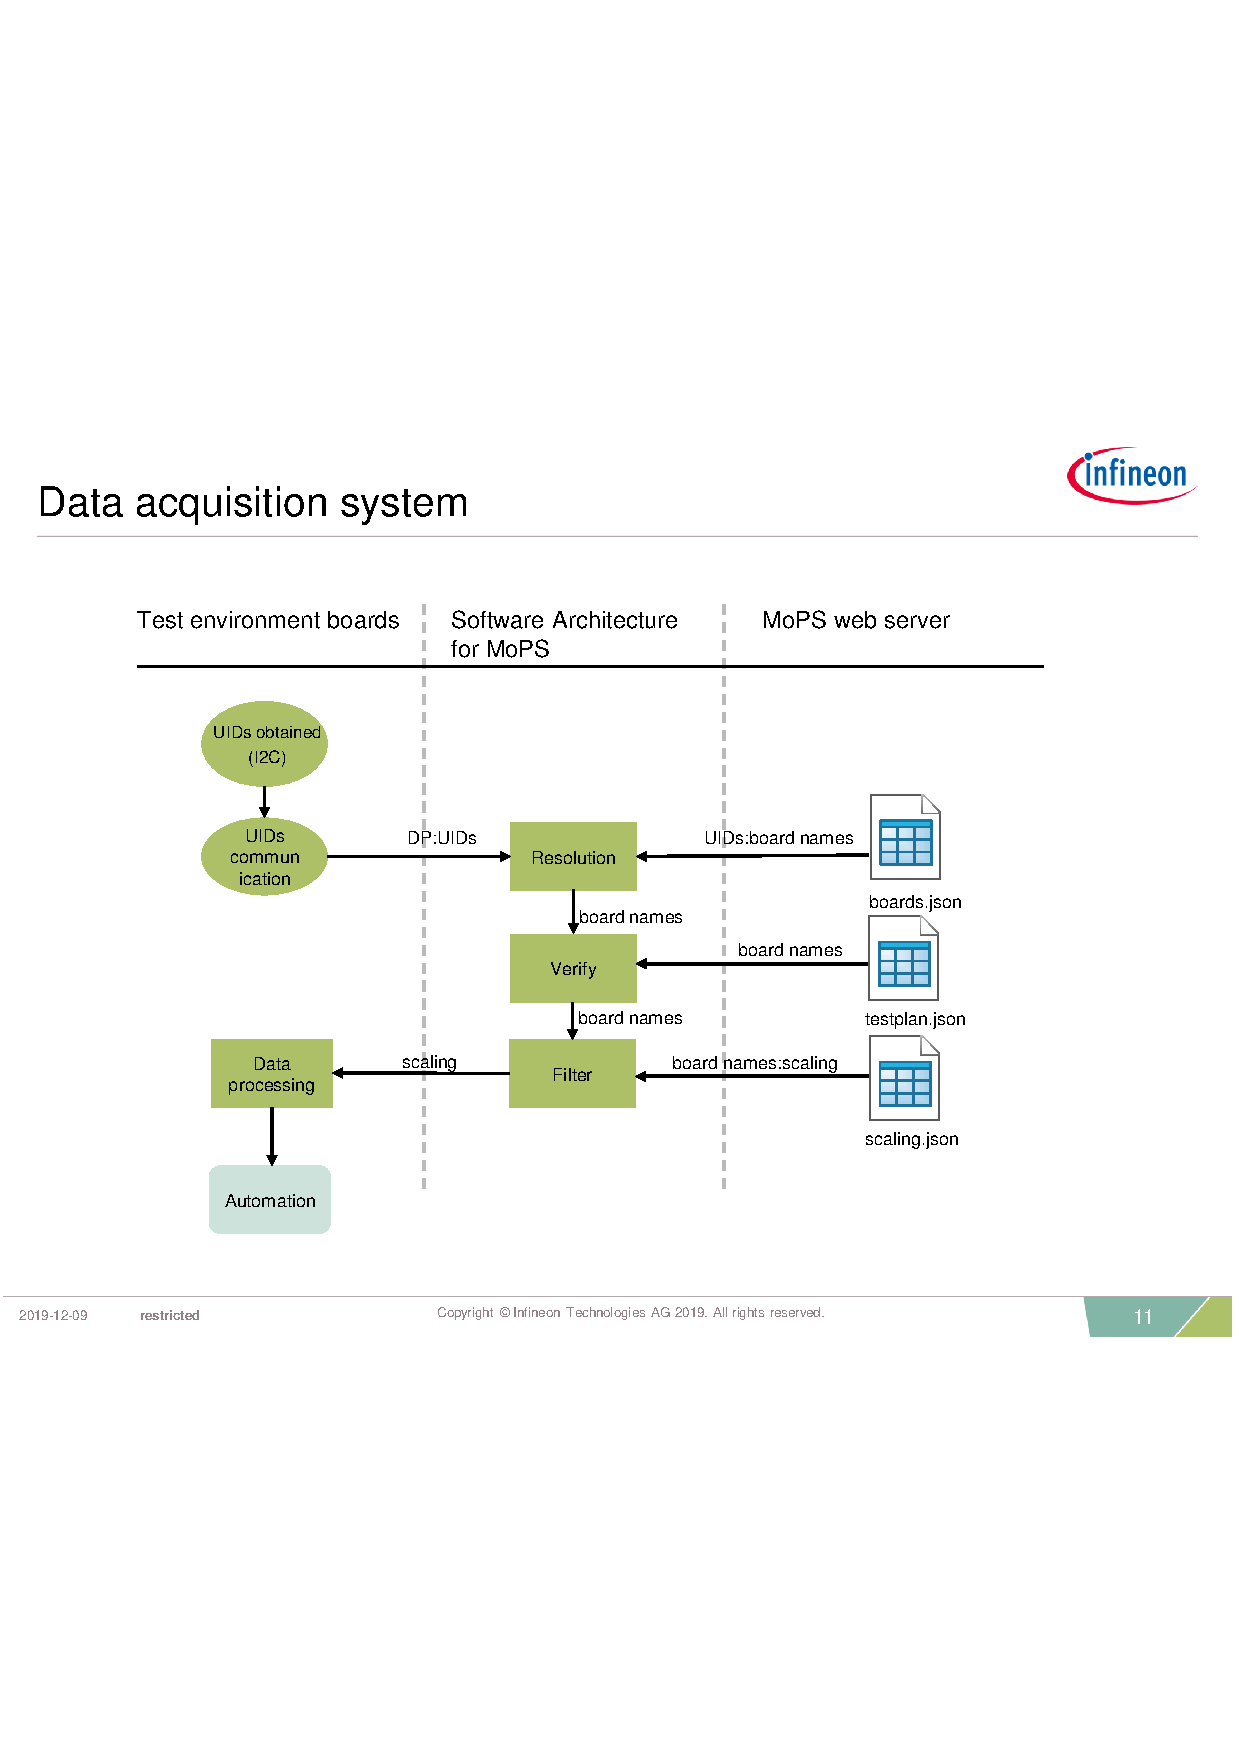
\includegraphics[trim=0 250 0 260, clip, width=160mm]{images/resolution.pdf}
		\caption{Resolution of board UIDs and scaling values communication}
		\label{fig:resolution}
\end{figure}
The board names that are fetched after the resolution of the board UIDs, are further authenticated with the board names that are present in the test plan. 
The board names that are present in the test plan are the hardware information provided by test engineers. 
Verification of boards are done in order to maintain consistency between the actual board connections and the test engineers selection of boards in the test plan. %In the perspective of this project, the board connections of Low Voltage MTS is as shown in the figure\cref{combination} and the respective test engineers hardware selection should be as shown in the ovenplan window(see Section \cref{TP}) of test plan.     
%Test engineers select the boards that are appropriate to the type of stress test that they are interested in conducting.
After the successful verification of board names in SAM, the verified board names are searched in the scaling connected \gls{LUT} to fetch the appropriate MicroMoPS channels and their scaling values.  

\subsection{Send the scaling values to MicroMoPS.}\label{sec:send}
The fetched communication channels and their corresponding scaling values are sent in queue as a string back to data processing system of MicroMoPS, using Ethernet communication.
The communication channels and their scaling values that are received at scaling related receiver handler of MicroMoPS are dynamically parsed to appropriately adjust the scaling values to the channels specific scaling variables (see \cref{lst:code_scaling}).
\subsection{Execute Low Voltage Test System}\label{sec:LowVoltage}
After successful adjustment of the scaling parameters in the MicroMoPS, the test sequence which is forwarded by SAM is executed on MicroMoPS. 
Finally, after all the above phases, the linear scaling mechanism and the Reverse Polish Notation get successfully integrated into the data processing system of MicroMoPS. 
The entire procedure of resolving the board UIDs supports to the automation of processing of analog measurements in MicroMoPS.
Measurements that are processed using linear scaling and Reverse Polish Notation are acquired at SAM and manipulated to retain the original values of analog measurements for any interpretation.
  
\afterpage{\null\newpage}
\afterpage{\null\newpage}
\afterpage{\null\newpage}
%\cleardoubleplainpage
\chapter{Implementation and Realization}
The discussed approach is brought into existence in this sophisticated test environment by accessing MicroMoPS and its peripherals, by extending the pre-developed MicroMoPS firmware and by effectively utilizing the Actor framework of SAM. 
The implementation of the proposed approach is done for a Low Voltage stress test system. 
The boards that are associated with the Low voltage stress test system (\cref{fig:combination}) are termed in the MoPS environment as follows:
\begin{itemize}
	\item Application module - BuckMoPS
	\item DUT module - LGA771
\end{itemize}

%\begin{figure}
%		\centering
%		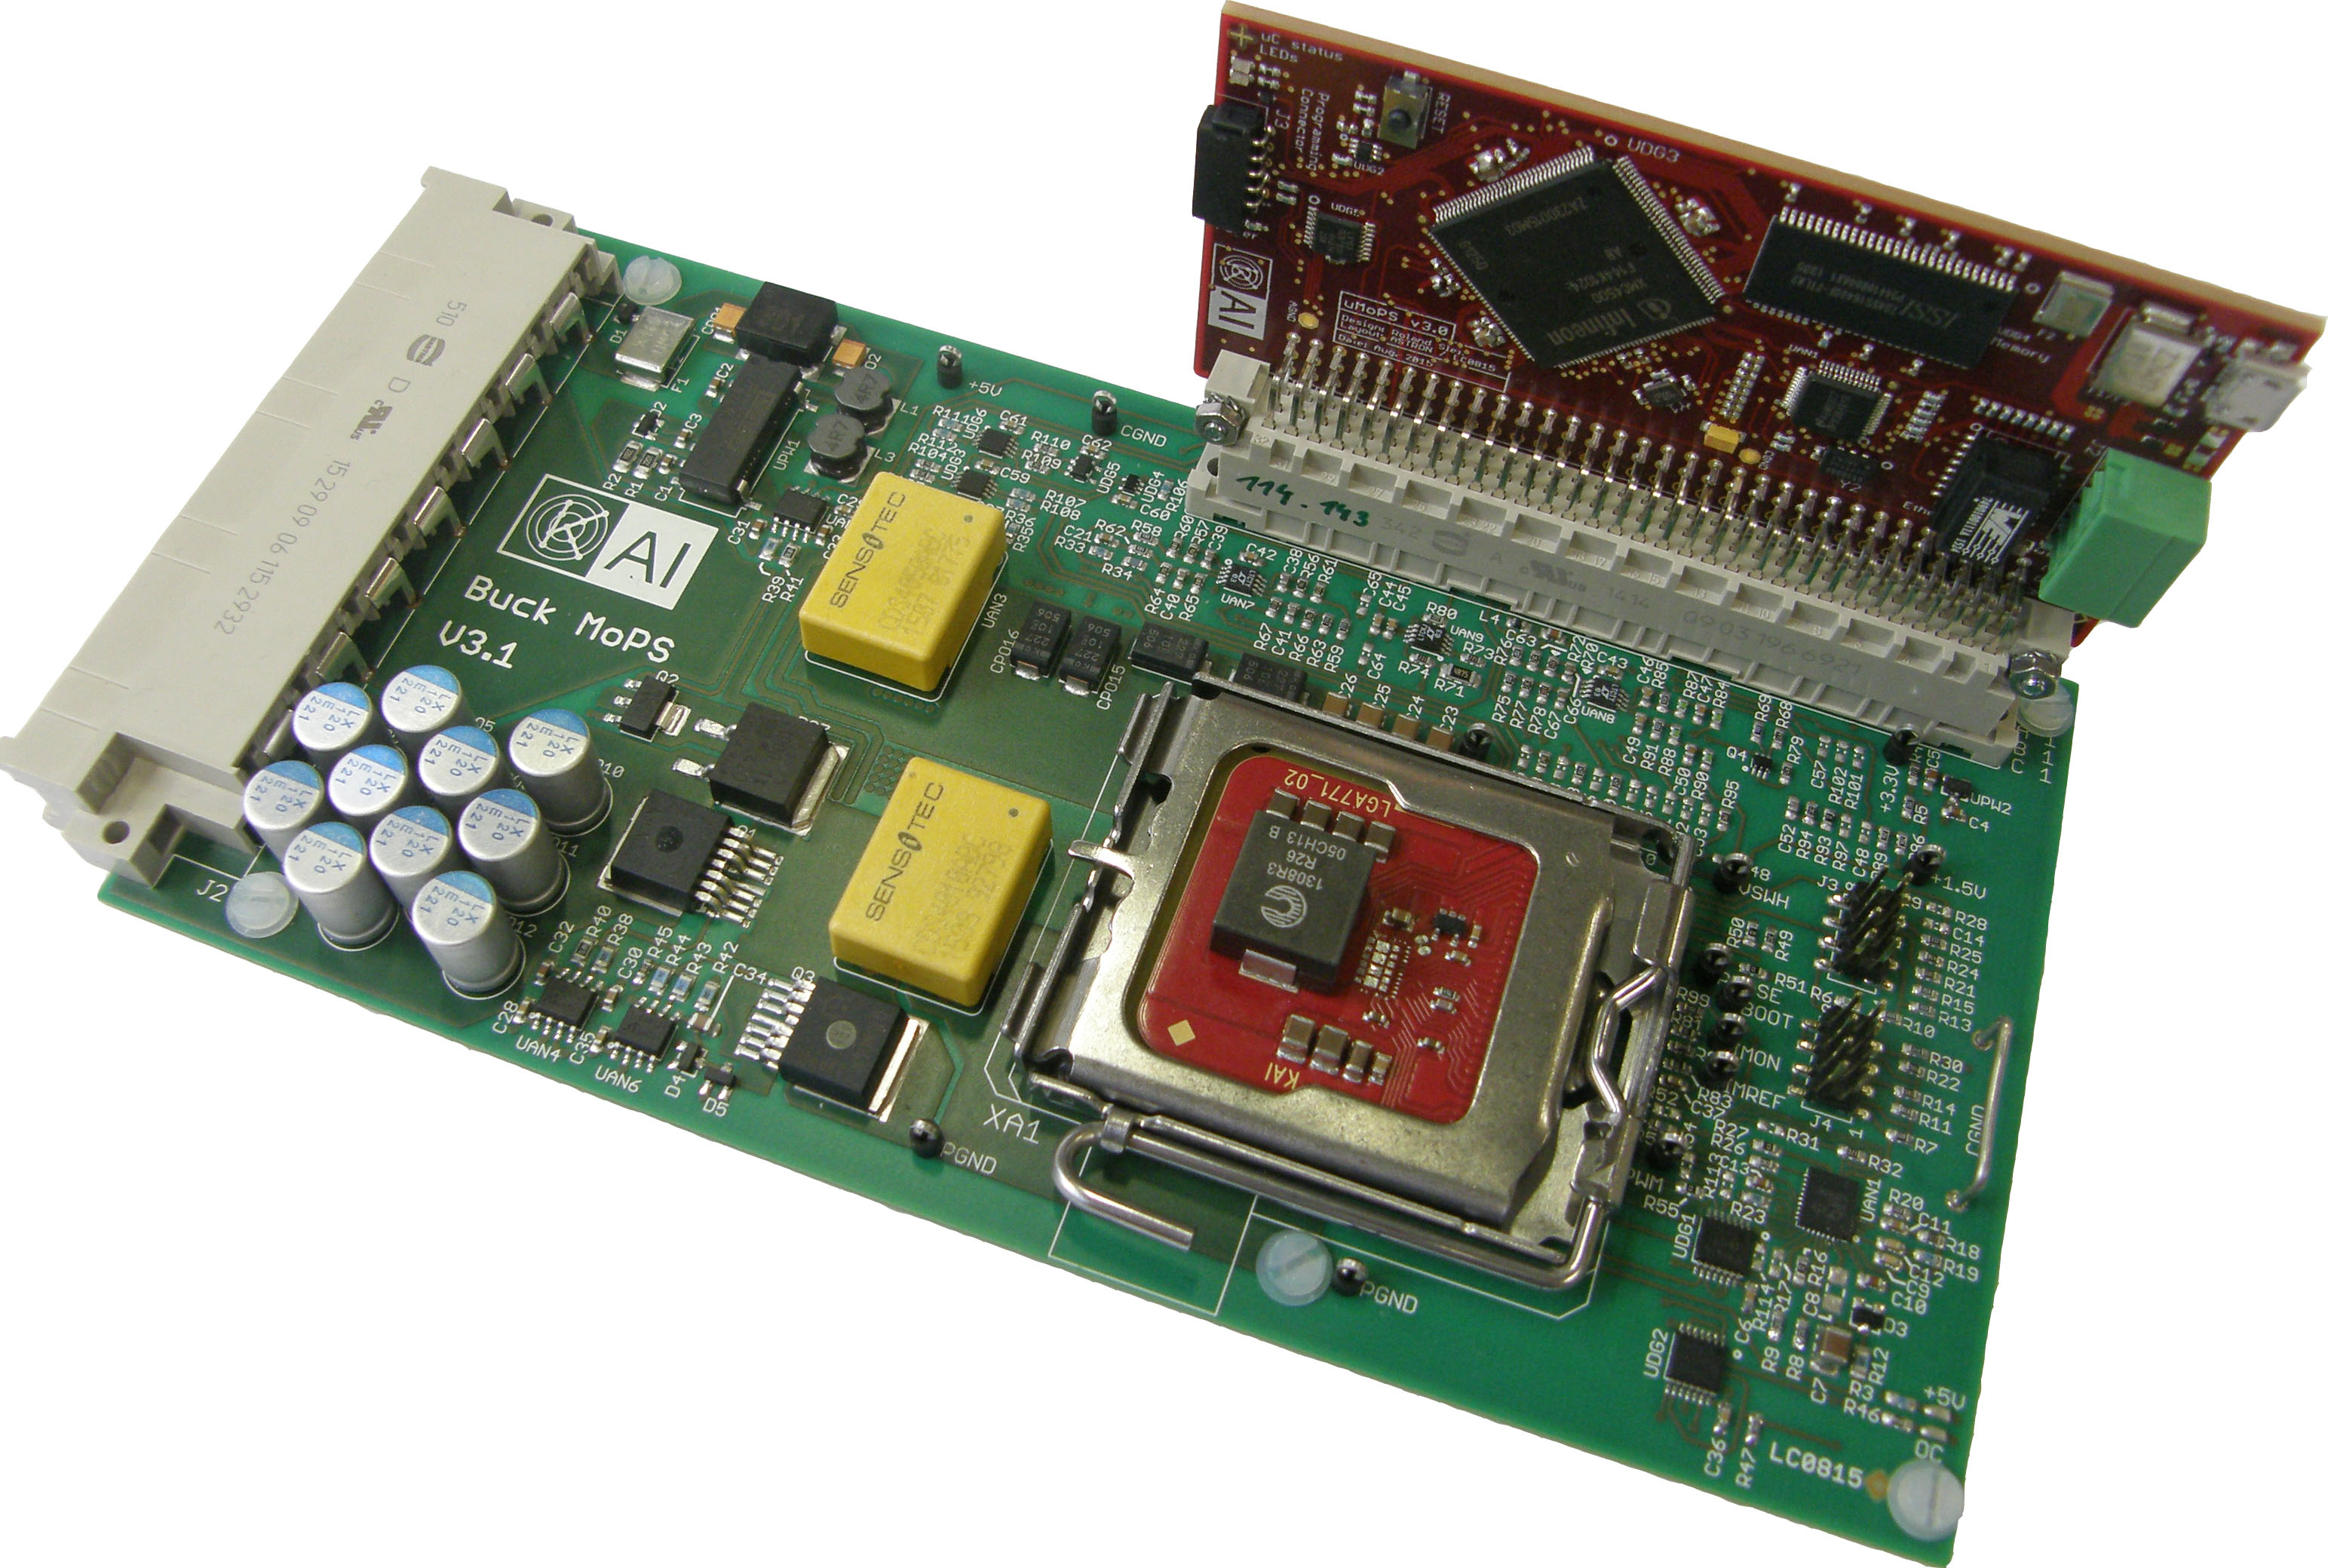
\includegraphics[trim=0 0 0 0, clip, width=100mm, scale=0.75]{images/Buck_and_uMoPS_2.jpg}
%		\caption{MicroMoPS, BuckMoPS and LGA771 arrangement.}
%		\label{combination}
%\end{figure}

\section{Extraction of UID of DUT and application board}\label{comm}
Board IDs are selected by using relevant \gls{GPIO} pins of MicroMoPS, which are meant for I2C (see \cref{sec:IIC}) communication.
In this work, MicroMoPS is treated as a Master block, DS28CM00~\cite{Maxim-DS28CM00-2006a} UID chip of application module and DUT as slave modules.
The operation of reading the board UID is succeeded by initializing and utilizing accordingly the appropriate digital IO pin of MicroMoPS.
The digital pin corresponding to the Master Module is set to appropriate mode at the very beginning of the operation.
Setting digital pin into an appropriate mode drives the Serial interface clock input (SCL) (see \cref{sec:IIC}).
Two PCA9515A~\cite{PCA951A-2014} ICs are embedded in the BuckMoPS to facilitate the MicroMoPS in reading UID of application board and \acrshort{DUT} module. 
With the support of PCA9515A ICs and UID chip, the corresponding DUT and application module are interacted from MicroMoPS using I2C communication. 

Obtainment of the board IDs is primarily controlled as per the programmer's requirement by utilizing the select line of the UIN chip of BuckMoPS. 
PCA9515A ICs are part of UIN chip present in BuckMoPS, which facilitates accessing the DS28CM00 module.
When the select line is set as logic $0$, PCA9515A of application module is enabled, which further establishes communication between MicroMoPS and UID chip of application module. 
Application module's UID can be requested using this communication. 
Similarly, when the select line is chosen as logic $1$, PCA9515A of DUT is enabled, which further establishes communication between MicroMoPS and UID chip of \acrshort{DUT}. 
\gls{DUT}'s \acrshort{UID} can be requested using this communication. 
There are two communication lines which need to be synchronously used by the master to write to UID chip or read from UID chip. 
They are, \acrshort{SDA} and \acrshort{SCL} lines (see \cref{sec:IIC}). 
SDA line is used for sending the data from master to slave or receiving the data from slave to master and SCL is used for providing synchronization in communication between master and slave. 
Because the concern is to read the board id of DUT and application module from MicroMoPS, systematic sequential communication procedure is followed (see \cref{sec:IIC}).
The received data is CRC verified using standard 8-bit polynomial i.e X8 + X5 + X4 + 1 \cite{Maxim-DS28CM00-2006a}, to authenticate the corruption of received data.

The above operation is implemented inside the test\_identify\_boards() handler (see \cref{sec:CORE}) of MicroMoPS firmware to successfully extract the board UID of BuckMoPS and LGA771.

The board \glspl{UID} extracted from slave devices are listed in the \cref{Table4}:

\begin{table}[ht]
	\centering
	\caption{Boards and their respective UID}
	\label{Table4}
	\begin{tabular}{|p{2.3cm}||p{3cm}|p{3.5cm}|p{2cm}| }
		\hline
		\textbf{Board type} &\textbf{Board name}   &\textbf{Unique Identity Number}    &\textbf{Select line}\\
		\hline
		Application module	&BuckMoPS   & 0x0d8d3c7   &0 \\
		Device under test &LGA771   	& 0x1052523   &1\\
		\hline
	\end{tabular}
\end{table}

\section{Update the microcontroller's configuration file for linear scaling computation}\label{resn}
The configuration file of a MicroMoPS contains the initializations of MicroMoPS associated peripheral modules. 
These modules are configurable based on the firmware developer's needs.
In the MicroMoPS firmware project, there is a dedicated configuration file to manage the configurations of a MicroMoPS called "config.c".

%\section{Update the configuration of MicroMoPS to integrate linear scaling mechanism.}\label{sec:configuration file}

%Could be included in implementation section
%Mathematically, obtained linear scaling mechanism is incorporated to processing of analog measurements in MicroMoPS, by updating the configuration of MicroMoPS. Scaling dependent structure in the configuration file of MicroMoPS is updated by appending linear scaling parameters for every communication channels of MicroMoPS. Updating, the configuration intuitively means that linear scaling variables can be used for digital data processing via a firmware module. EDS is also generated upon microcontroller booting (see Section\cref{CORE})

To incorporate the linear scaling mechanism to MicroMoPS, the scaling module i.e MoPS scaling, is extended by adding two parameters as shown in the \cref{lst:code_scaling}.
The added parameters are \emph{scaling factor} and \emph{offset} in adjacent to the respective analog channel (.name) parameter.
The scaling values that are assigned are the default scaling values.
These values are meaningful to measurement circuits of the Low-Voltage stress test system.
These scaling values are updated automatically with different values when the stress test system that is performed is different from the Low-Voltage test system.

The \gls{EDS} is generated every time when the MicroMoPS firmware starts. 
The EDS contains the communication channels and channels' specific scaling parameters. 
The \acrshort{DUT} creation in the mops web server based on the EDS information and downloading of the \glspl{LUT} when SAM starts running was carried out by summer students of KAI.

%\begin{listing}[htp]
%	\inputminted[frame=single]{C}{src/scaling.c}
%	\caption{MoPS scaling}
%	\label{lst:code_scaling}
%\end{listing}

\lstinputlisting[frame=single, label=lst:code_scaling, caption=MoPS scaling, firstnumber=1]{src/scaling.c}

\section{Board UIDs communication to SAM}
		 The byte-wise data of \gls{UID}, which are received from the \gls{UID} chip is collected and combined inside test\_identify\_boards() (see \cref{sec:CORE}) handler to reproduce UID (64-bit length) of the board. 
		 In this work, UID of BuckMoPS and LGA771 are restored.
		 The restored UIDs are further communicated to SAM using the dedicated MicroMoPS' test handlers~\cite{Steinwender2016}.

\section{Resolution of UIDs in SAM and scaling values communication from SAM to MicroMoPS}
The resolution of Board IDs in SAM is implemented by utilizing the LabVIEW software packages. 
\begin{figure}[hbt]
		\centering
		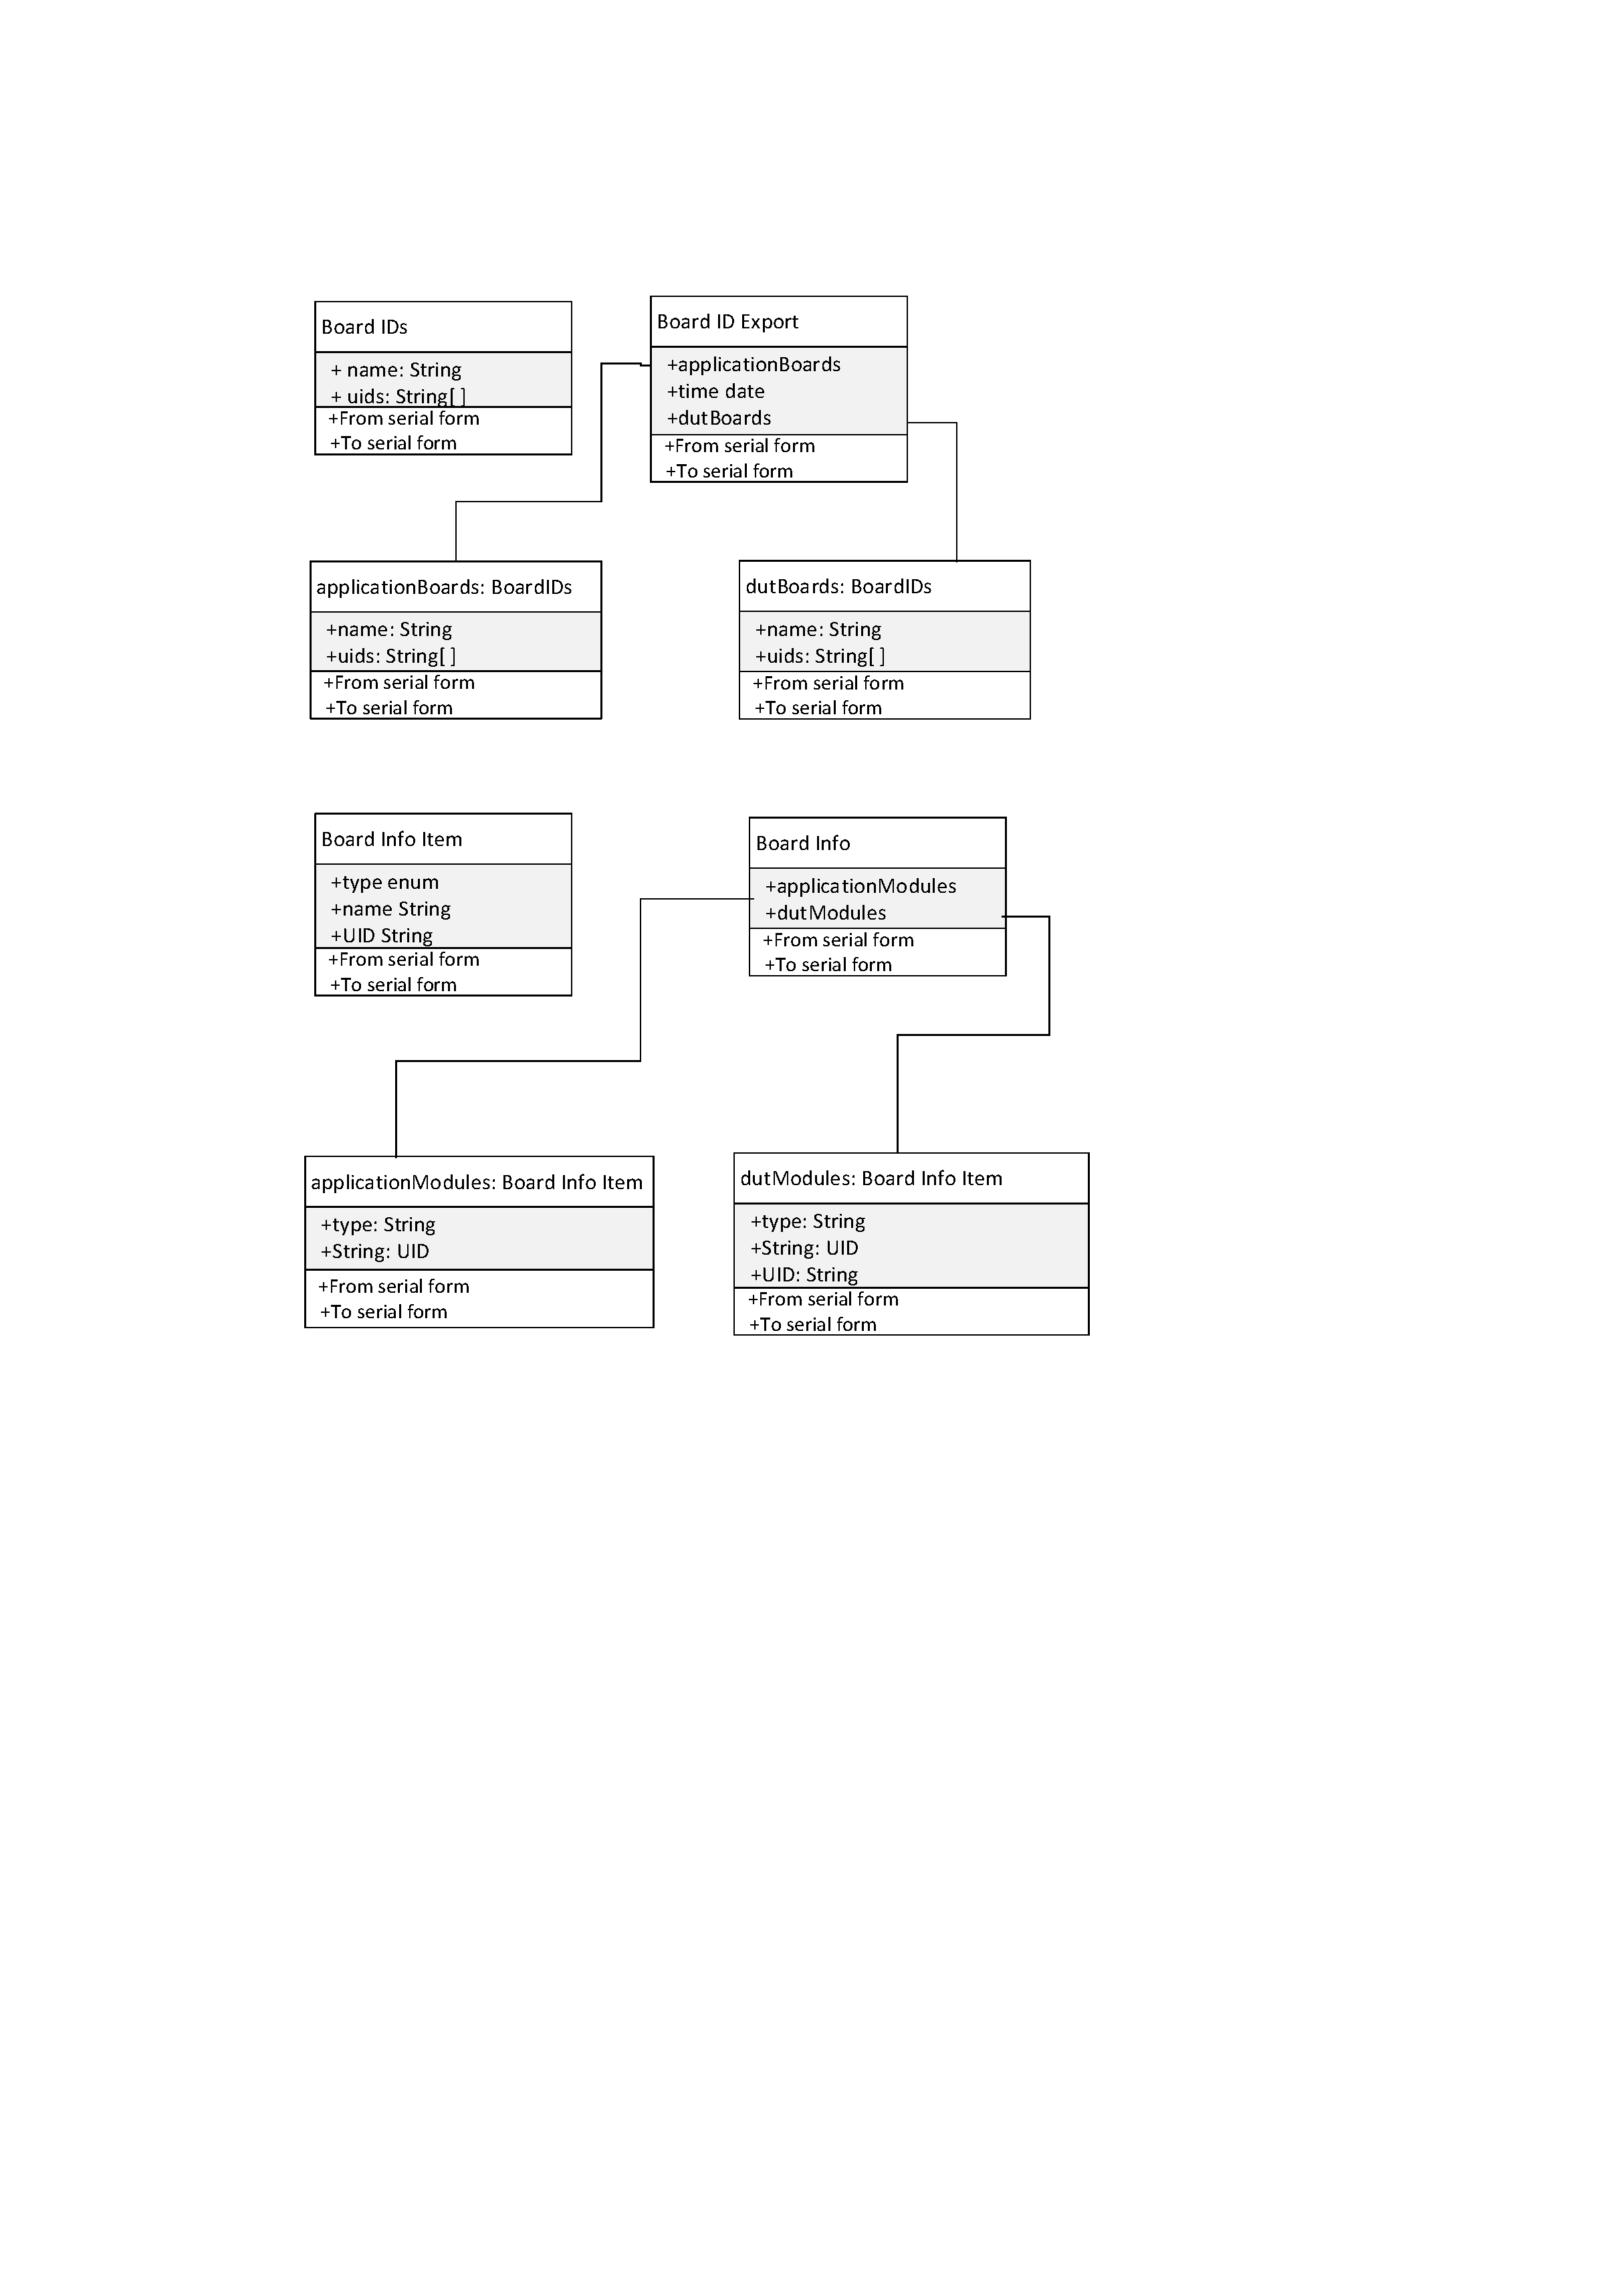
\includegraphics[trim=180 670 0 140, clip, width=210mm, scale=0.75]{images/board_objects.pdf}
		\caption{Serialization of JSON objects into LabVIEW data structures}
		\label{fig:Serialization}
\end{figure}
The basic step before the implementation of the algorithm which mainly resolves the board ids is the serialization of the application module's objects and dutBoard's objects into LabVIEW data structures as shown in the \cref{fig:Serialization}.
The application module's objects and the dutBoard's objects are present in the "boards.json".
The board UIDs are cached offline using I2C communication and communicated to SAM.
The derived scaling values and board UIDs are stored in a database of \acrshort{MoPS} web server.
As described in the \cref{sec:uidResolution}, the board database, and scaling database are downloaded by SAM from the MoPS web server. 
Intuitively, "boards.json" and "scaling.json" are downloaded by the main actor of SAM to facilitate the board UIDs resolution. 
The resolution of board UIDs is done in the Node actor (see \cref{sec:SAM}) of SAM. 
To achieve board UIDs resolution, variables such as "name" and "uids" are declared as string and array of string data members of class "Board IDs", respectively as shown in the \cref{fig:Serialization}. 
Similarly, variables such as applicationBoards and dutBoards are declared as data members of "Board ID export" class.
The data members of "Board ID export" i.e applicationBoards and dutBoards, are an instance of the class "Board IDs".
%The serialization of the JSON objects i.e application module and dutboard, is to unflatten the lists present in these JSON objects into LabVIEW variants.

The classes that are created by the name "Board IDs" and "Board ID export" are the LabVIEW classes.
The serialization methods that are present in the classes do the conversion of JSON objects present in "boards.json" into strings. 
These strings are nothing but the key-value pair of applicationModule and dutBoard as shown in the \cref{lst:boards}. 
Thus, by means of serialization, the board name and uid values of applicationModule JSON object and dutBoard JSON object are assigned to applicationBoards and dutBoards data members of "Board ID export", respectively.
In the same way, the board UIDs along with their directional pin that are received by SAM from MicroMoPS, are assigned to data members of "Board Info item".
Based on the directional pin value, the received board UIDs are classified into appropriate board type and accordingly, the board UIDs are assigned to UID data member of "Board Info item".
After a successful serialization, the UIDs of data members (applicationBoards and dutBoards) of "Board Info item" are compared with the UID of data members (applicationModules and dutModules) of "Board ID export".

\begin{figure}[hbt]
		\centering
		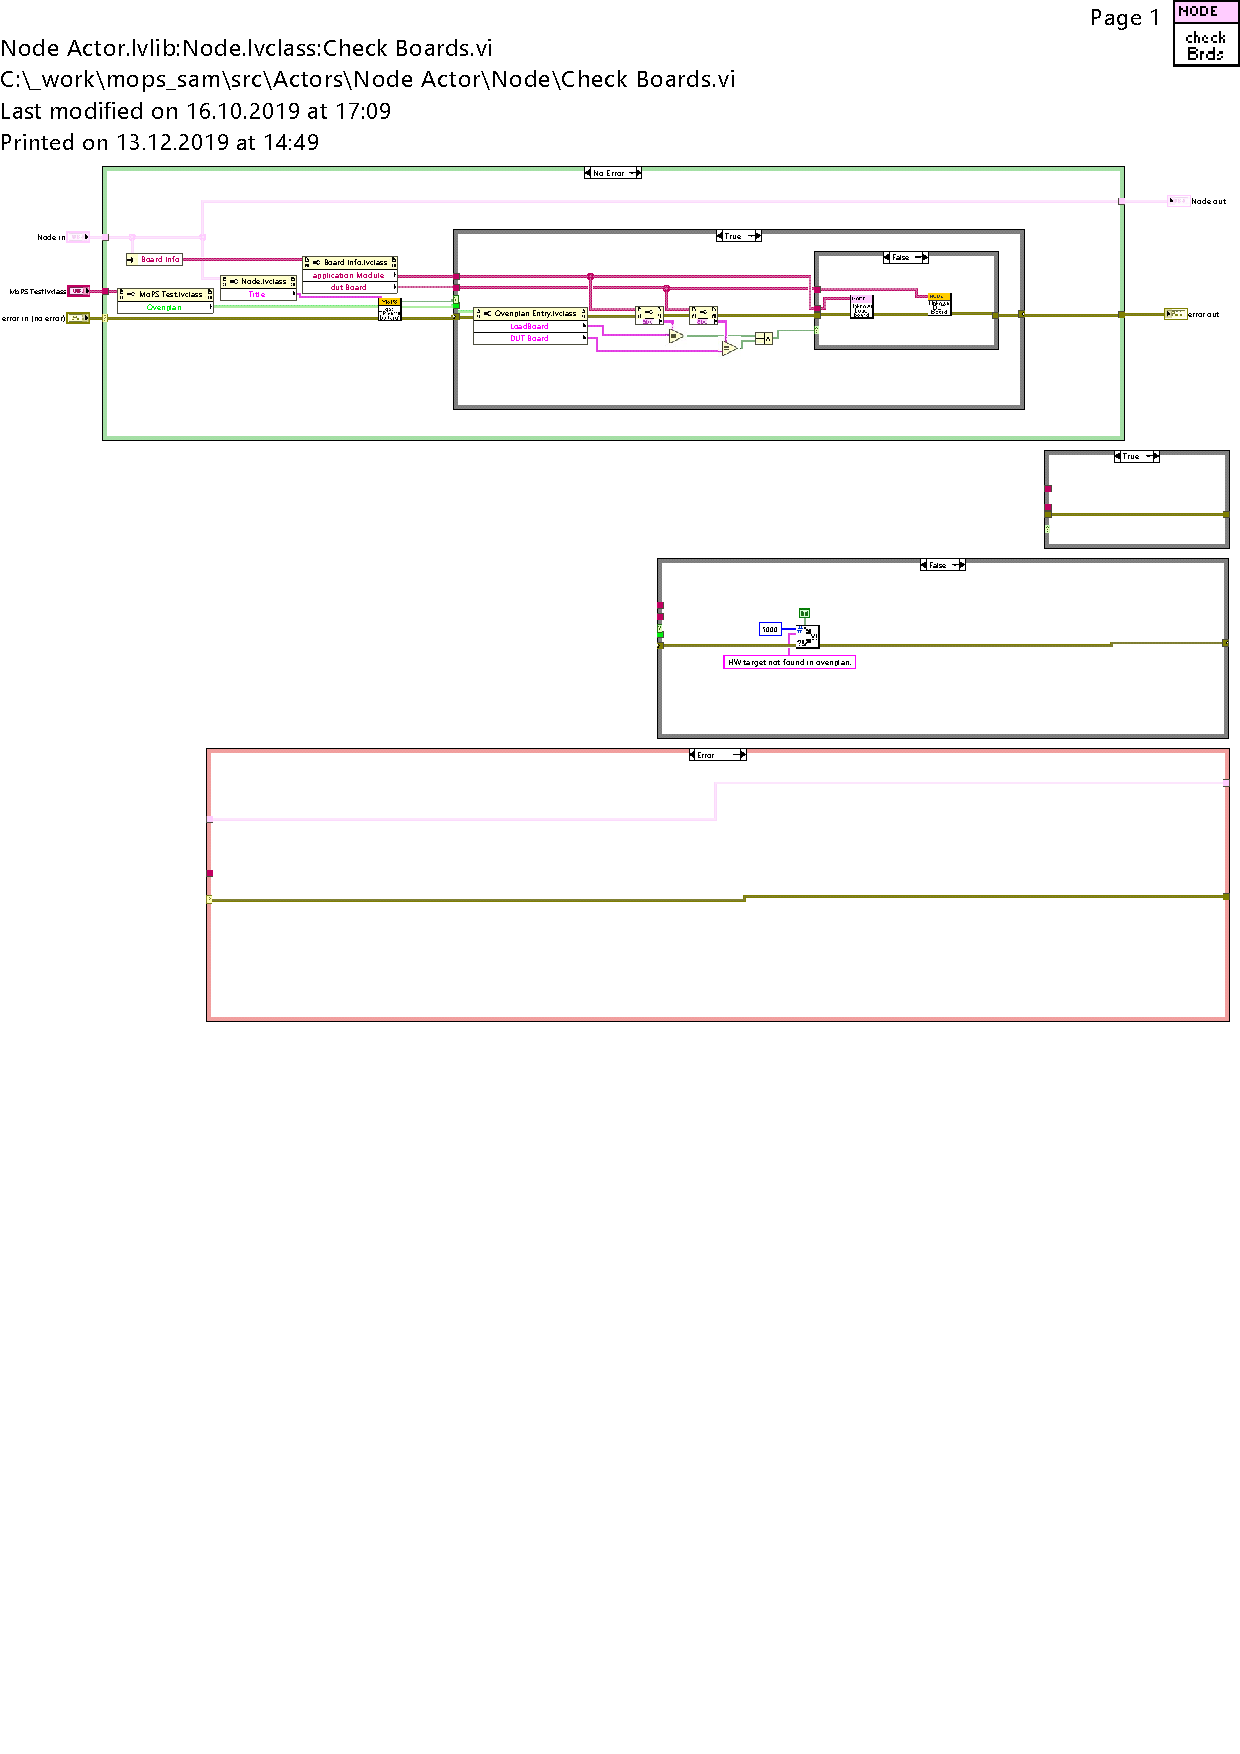
\includegraphics[trim=0 628 0 80, clip, width=155mm, height=70mm, scale=3]{images/verify.pdf}
		\caption{Verification of boards with oven plan entry.}
		\label{fig:Verify}
\end{figure}

This, comparison if found matched, the respective board names such as BuckMoPS and LGA771 are updated to application module and dutModule objects which are instances of "Board Info". 
Earlier to this update, only a UID information and the type was known to application module and dutModule objects, through the MicroMoPS communication. 
Successful comparison leads to the resolution of board UIDs. The updated board names along with their respective types in "Board Info" are logged on to the log GUI display of SAM.
Logging of board names with their type helps the test engineers or SAM developers to know the status of detection of boards by SAM.
%Explain algorithm in steps

\begin{figure}[hbt]
		\centering
		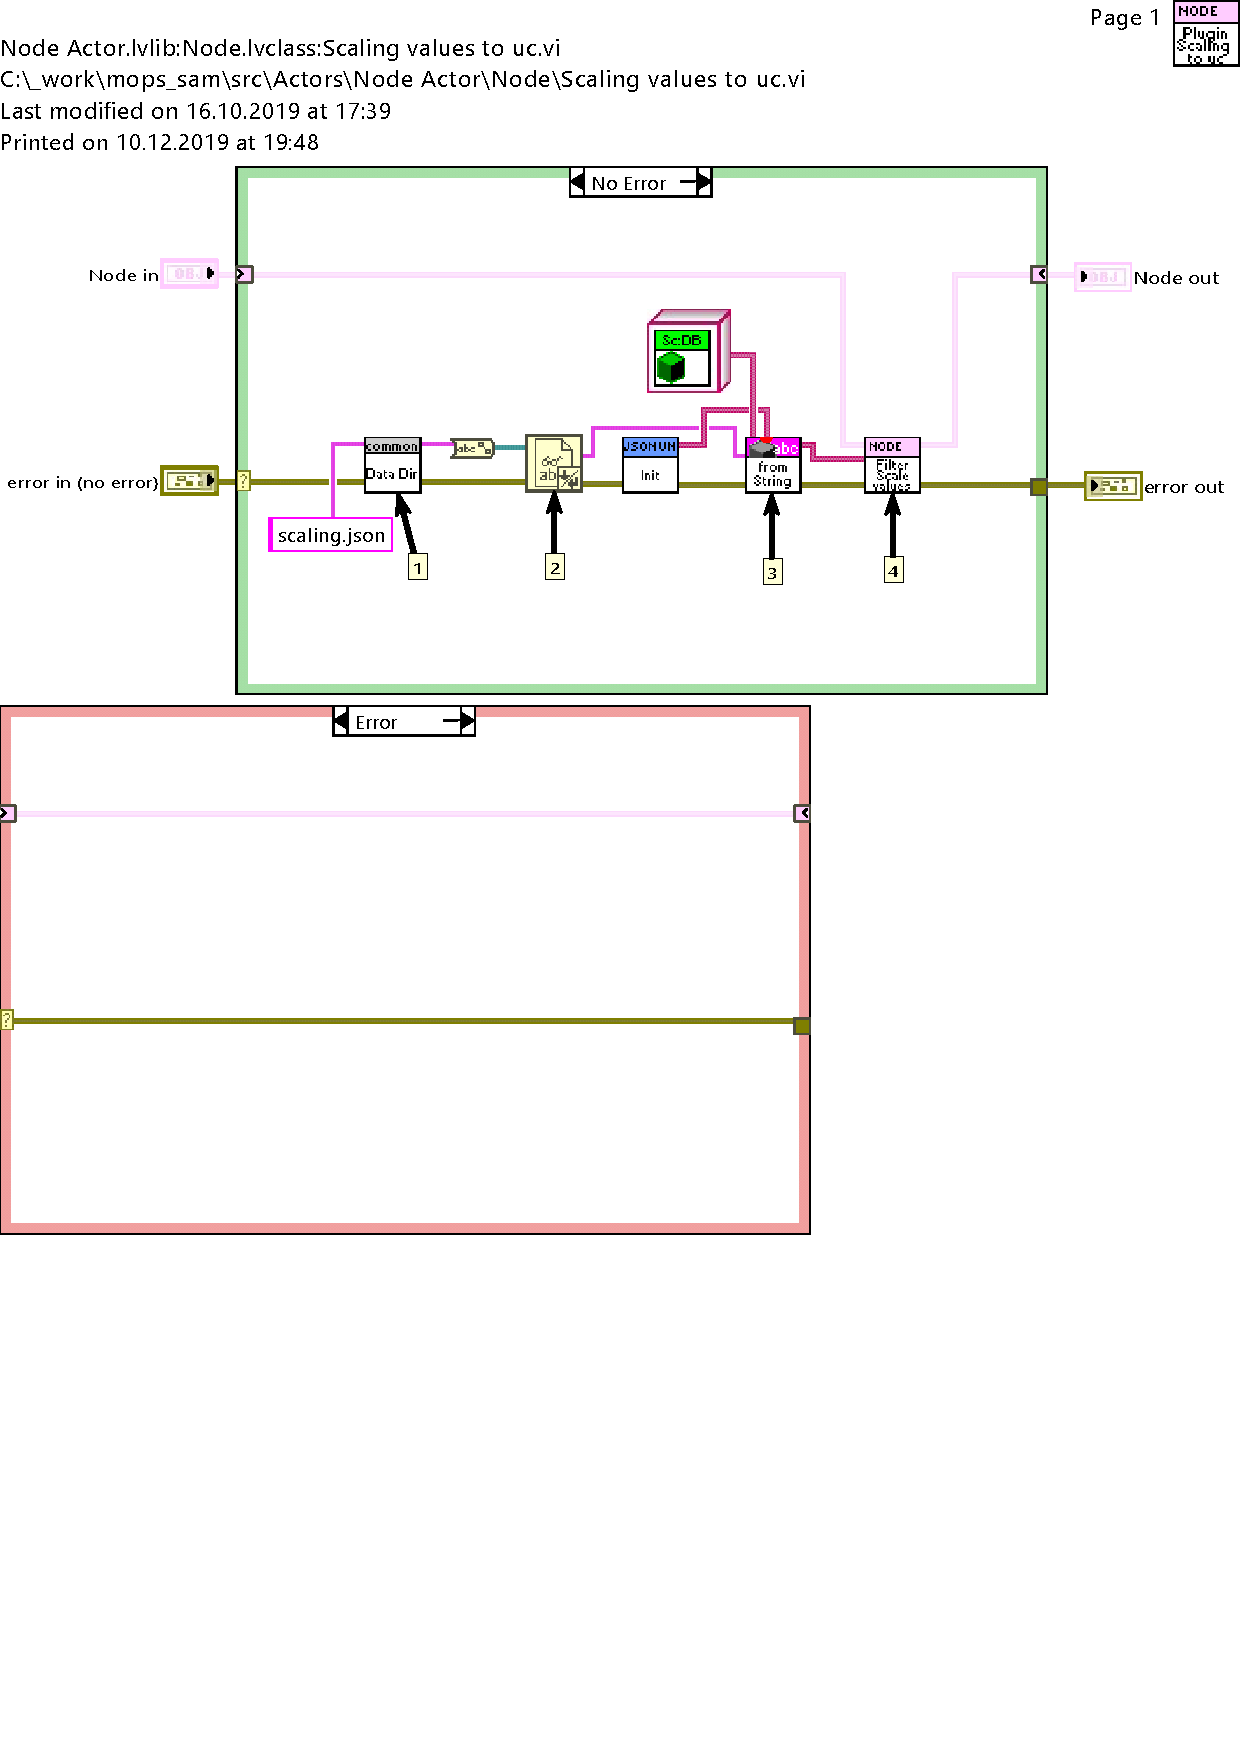
\includegraphics[trim=0 505 0 75, clip, width=150mm, scale=2]{images/Filterscalingvalues.pdf}
		\caption{Communication of channel name and associated scaling values to MicroMoPS.}
		\label{fig:Communication}
\end{figure}

Further, the board names that are present in the application module and dutModule objects are verified with the Hardware information present in the oven plan as shown in the \cref{fig:Verify}. 
The Serialization procedure as described earlier is undergone by test plan (JSON) to un-flatten the oven plan JSON objects into LabVIEW data structures. 
The Hardware information which is present in the oven plan entry class (due to serialization) is verified with the board names that are present in the application modules and dutModules.
If the verification is unsuccessful, the conflicting board information is reported to the MoPS web server. 

\begin{figure}[hbt]
		\centering
		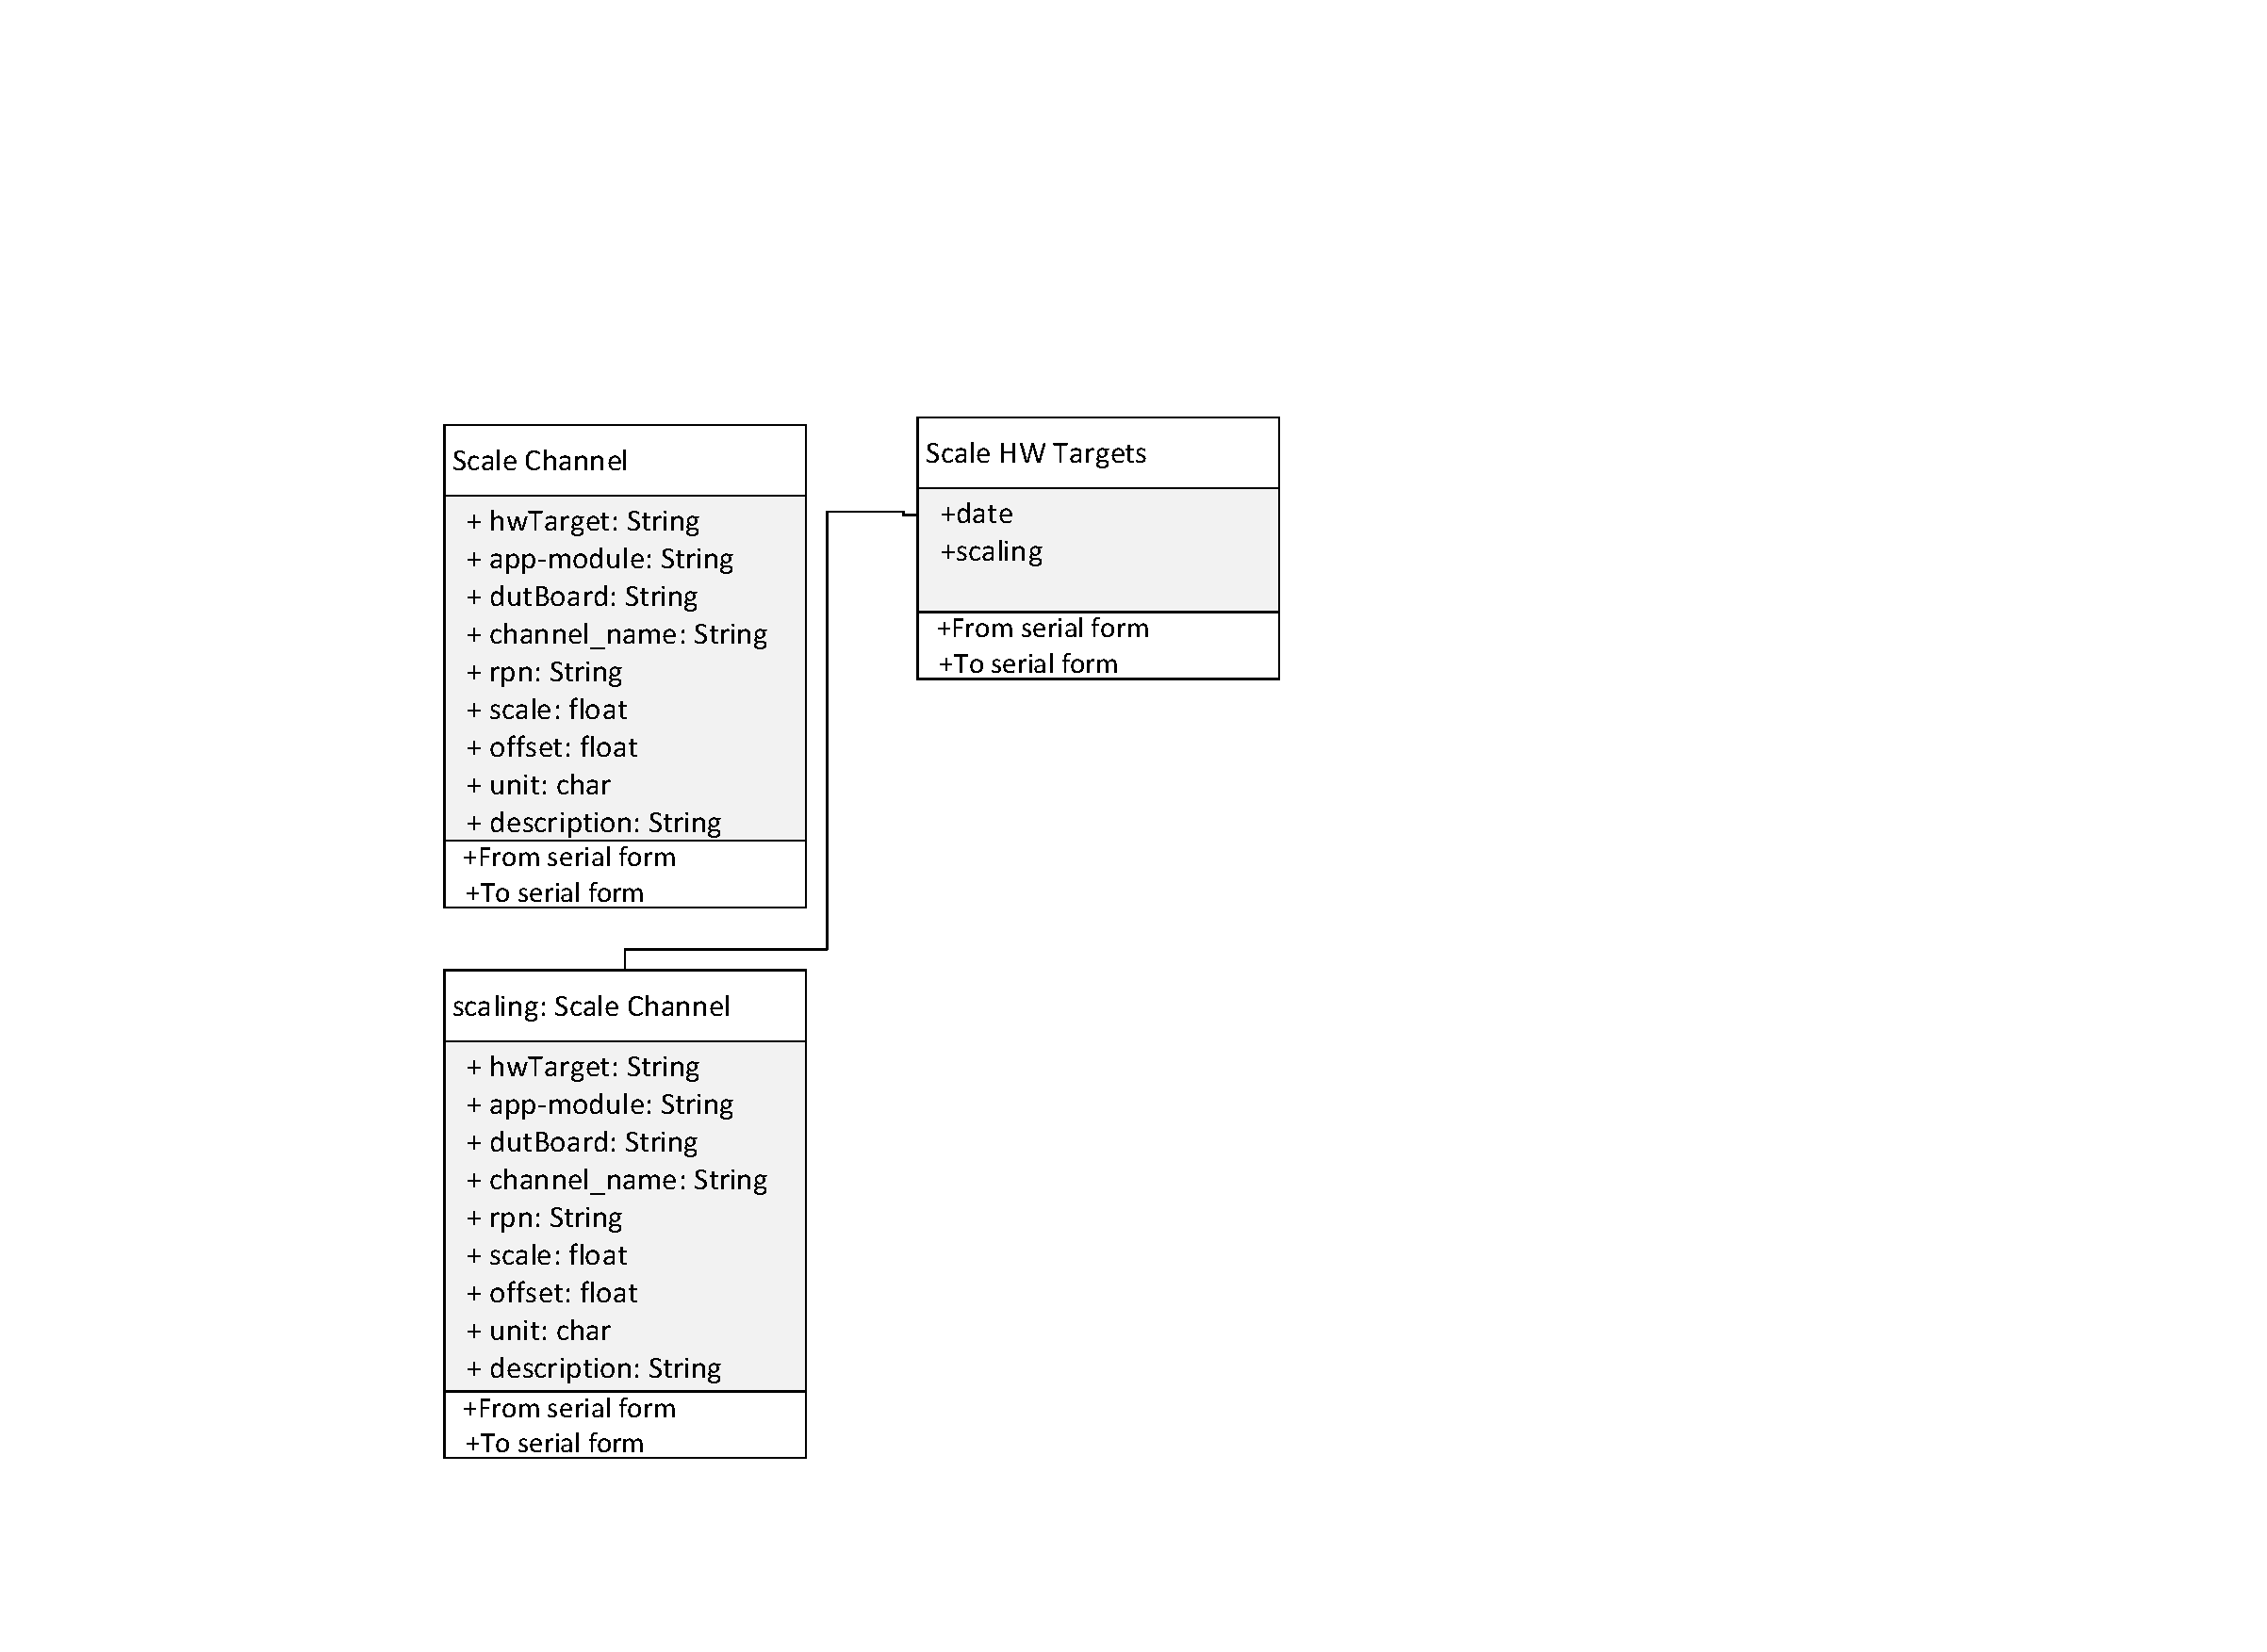
\includegraphics[trim=0 55 0 210, clip, width=210mm, scale=0.75]{images/Scaling_channel.pdf}
		\caption{Serialization of "scaling.json" objects into LabVIEW data structures}
		\label{fig:scSerialization}
\end{figure}

After successful verification, the board names correspondent combination is searched from the "Scale HW Targets" LabVIEW object. 
"Scaling" object is a result of serialization of "scaling.json" (\cref{fig:Communication}) into LabVIEW objects.
Serialization of "scaling.json" (\cref{fig:Communication}) into LabVIEW objects enables the conversion of JSON objects (\cref{lst:scaling}) present in the "scaling.json" into strings. 
After Serialization, filtering of channel names, scaling values and offset parameters, and communication of the same are done at a particular sequence as shown in the \cref{fig:Communication}. 
Below are the operations that are done at the mentioned sequence:       

\begin{enumerate}
\item Read the configuration path.
\item The text present in the text file is read.
\item De-serialization of JSON objects into LabVIEW objects is performed.
\item The data members of the "Scaling" object i.e Hardware Target, application module and \acrshort{DUT} board combination are compared with the applicationModule and dutModule objects. 
In the case of successful match, the board combination specific scaling value, offset and channel name are filtered from the "Scaling" object. 
The filtered parameters are further communicated to the board ID receiver handler~\cite{Steinwender2016} of MicroMoPS. 
\end{enumerate}

\begin{figure}[hbt]
		\centering
		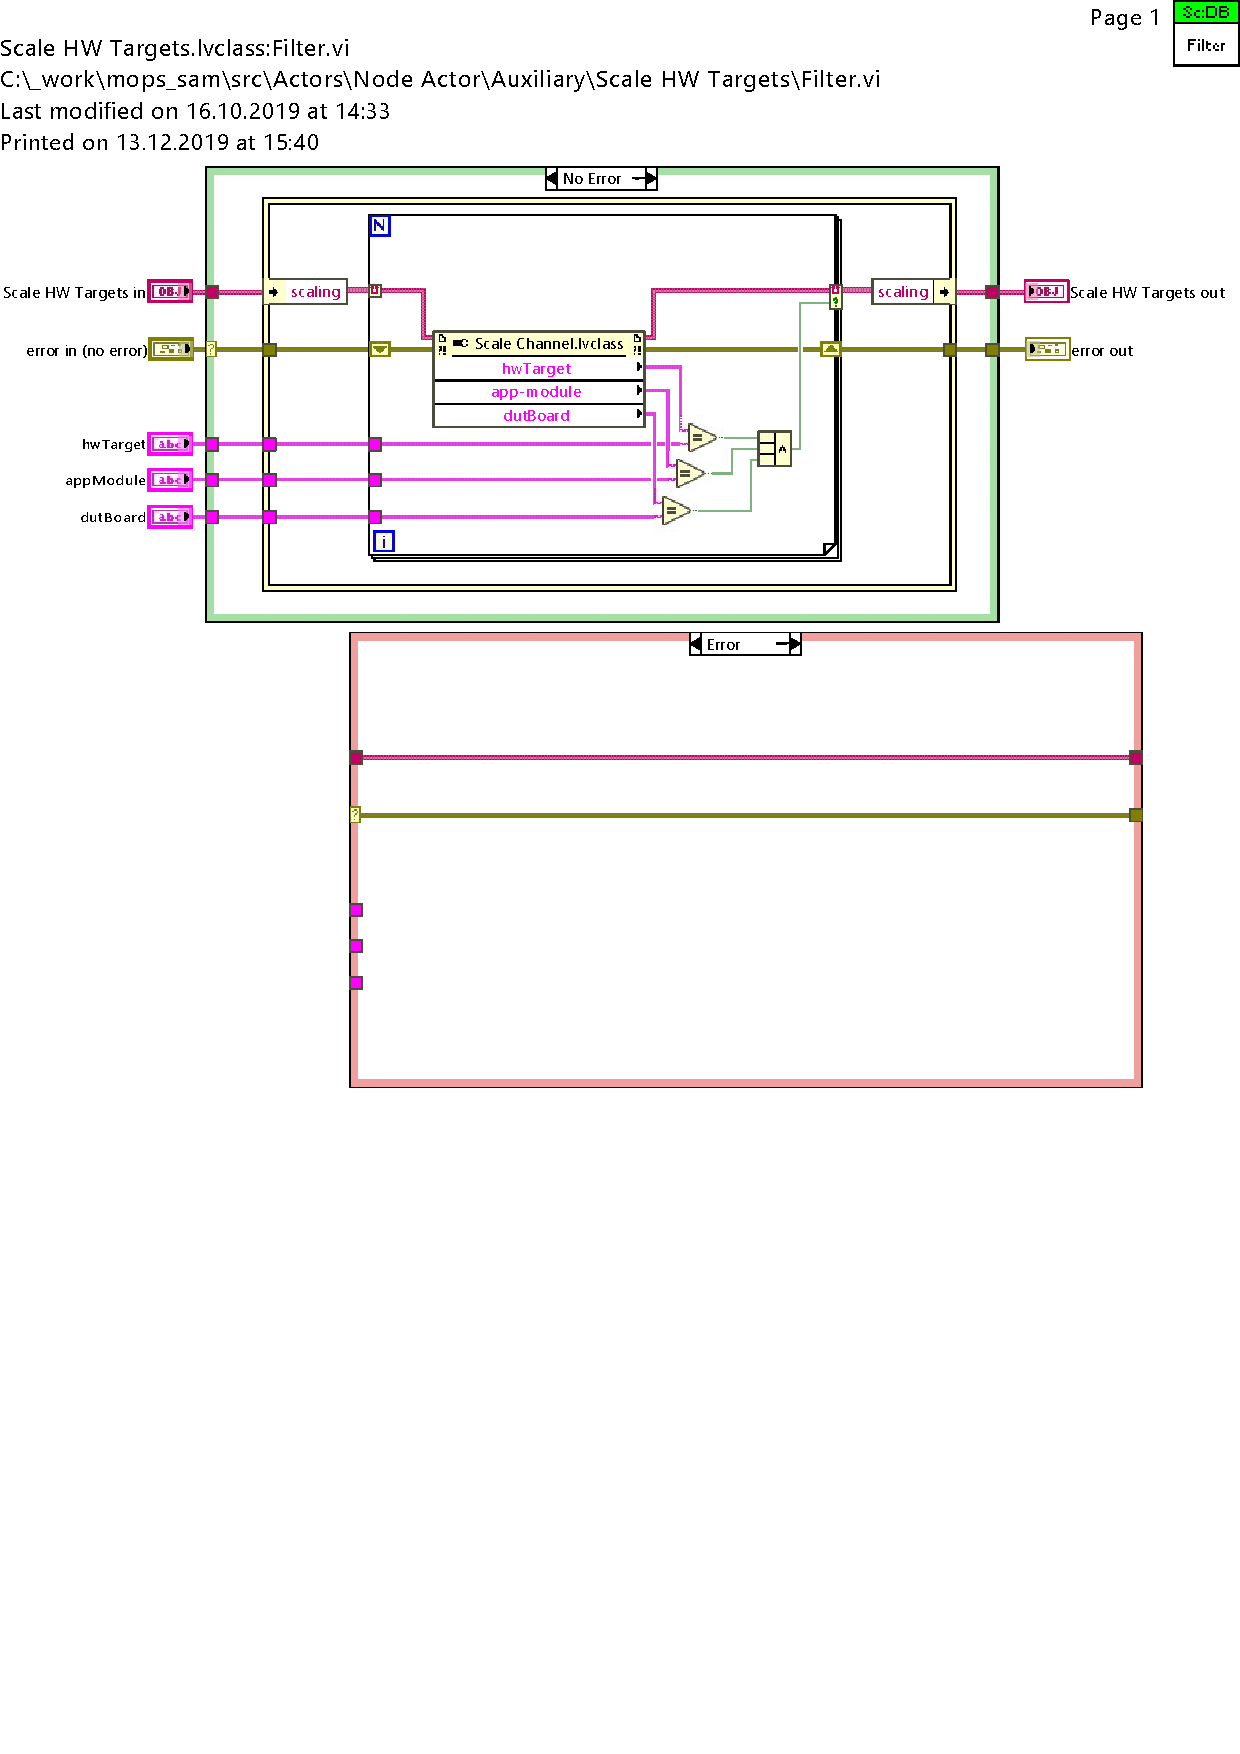
\includegraphics[trim=0 540 0 75, clip, width=130mm, scale=0.75]{images/filterVI.pdf}
		\caption{Filtering of scaling values}
		\label{fig:FOS}
\end{figure}

The filtering of the scaling values are implemented as shown in the \cref{fig:FOS}. 
The "Scaling" object is an instance of "Scale Channel" class which contains the hwTarget, app-module, 
dutBoard, channel\_name, rpn, scale, offset, unit and description data members. 
Data members such as scale, offset and channel\_name are filtered by performing a comparison between the board names that are obtained after resolution and the hwTarget, app-module and dutBoard data members, respectively. 
The control module's board name is obtained from the hardware information present in \acrshort{EDS}.   

\begin{figure}[hbt]
		\centering
		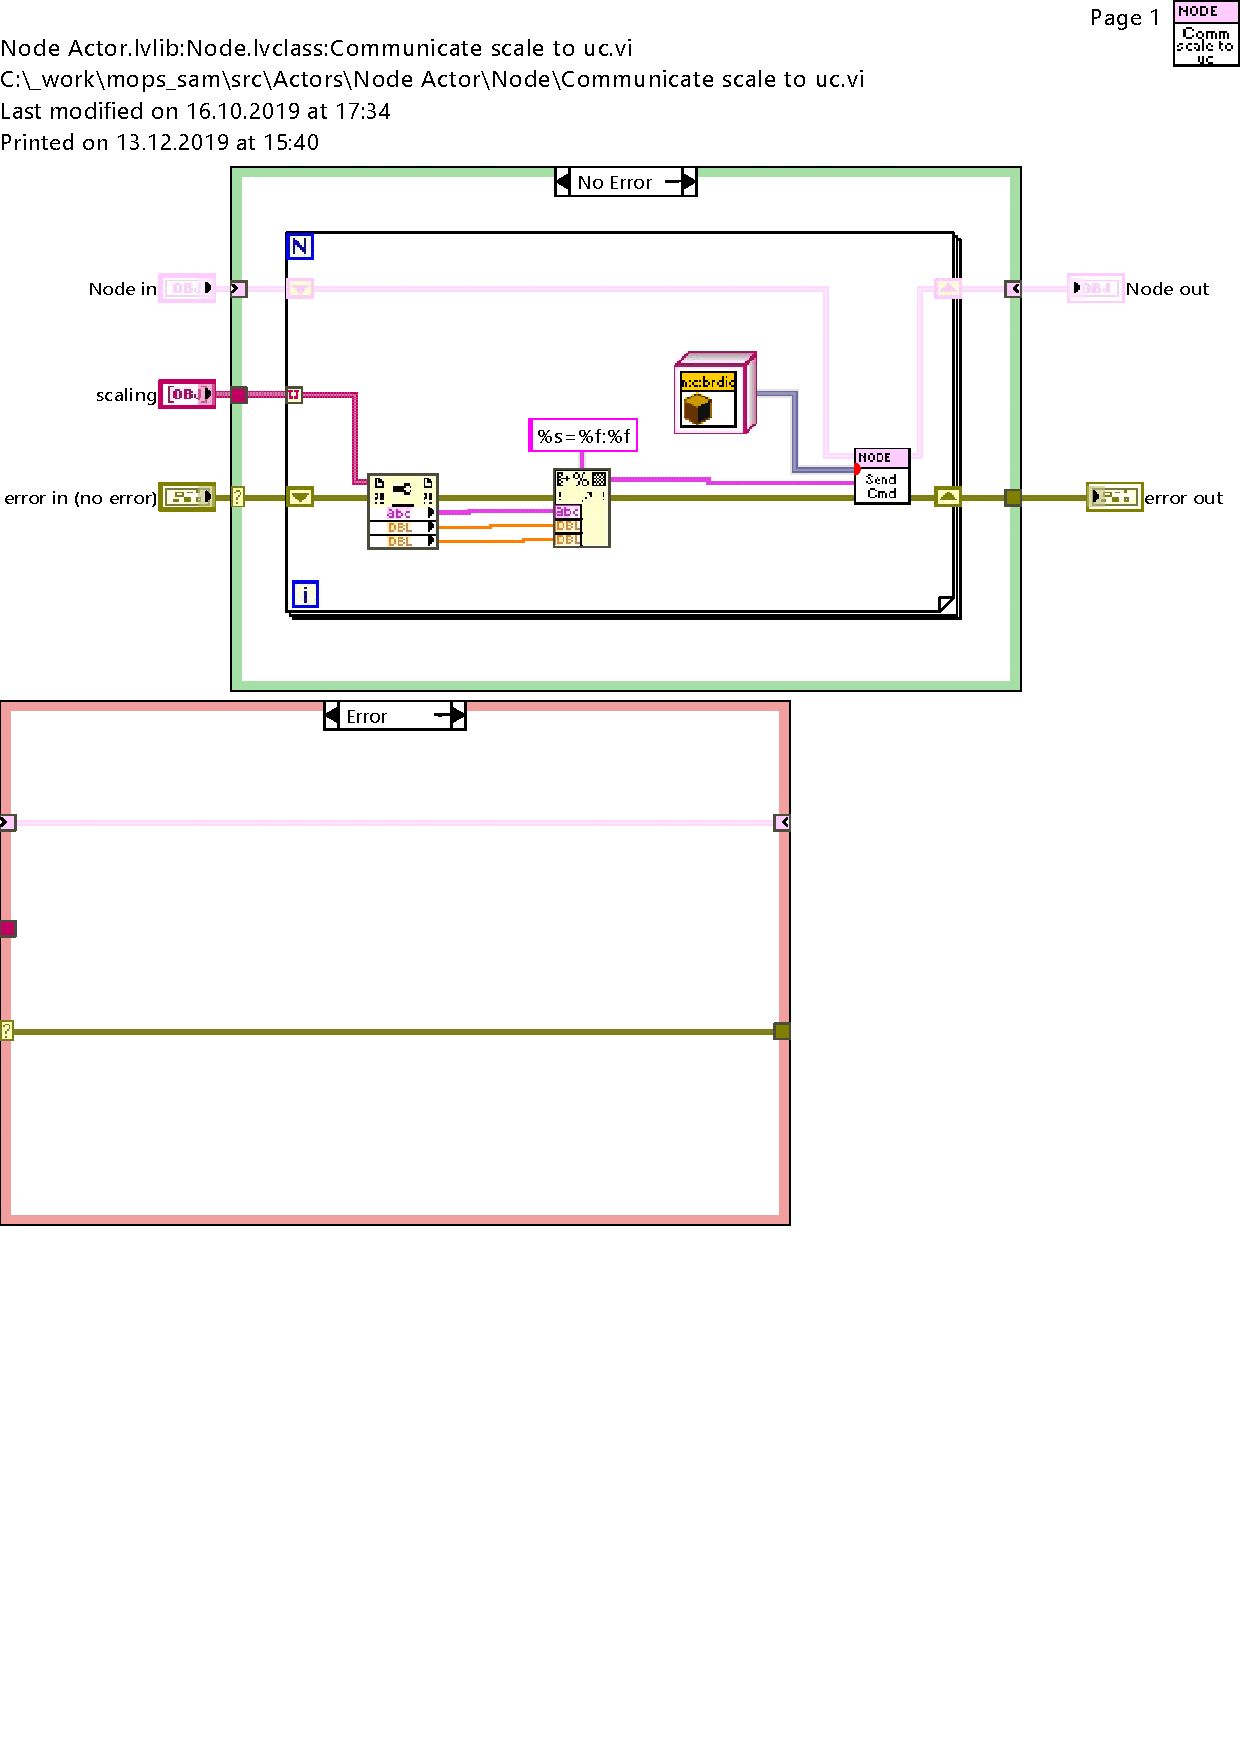
\includegraphics[trim=0 510 0 75, clip, width=130mm, scale=1]{images/commscaling.pdf}
		\caption{Communication of scaling values}
		\label{fig:COS}
\end{figure}


Finally, the filtered parameters are communicated to the board ID receiver handler of MicroMoPS. 
The filtered parameters are specific to every individual channel. 
The parameters are channel-wise communicated in a queue to MicroMoPS.
The \acrshort{VI} implementation of communication of scaling values is as shown in the \cref{fig:COS}.   

\section{Parse the scaling parameters dynamically in MicroMoPS}\label{sec:parse}
	Sequentially, the board combination specific communication channels and their respective scaling parameters are received as a payload (string data) from \gls{SAM} to board ID receiver handler (MoPS\_cmd\_handler\_BOARDID()) of MicroMoPS (see \cref{fig:DP}). 
	The string data that is obtained at board ID receiver handler of MicroMoPS is delimited by ':' between channel name and scaling parameters. It as shown in the example: "sync0:0B:0.0007326007326:0". 
	Where, sync0:0B is a channel name and module (see \cref{sec:Channels}), 0.0007326007326 is a value of the scaling factor denoted by 'k' and 0 is a value of offset denoted by 'd'. 
	This string is dynamically parsed and assigned to channel-specific scale (.scale) and offset (.offset) variables (see \cref{fig:DP}) present in the "MoPSscaling" module.
	Other parameters such as .func and .name are presesnt in order to define the RPN function and the communication channel module, respectively. These parameters are globally used in MoPS firmware, which are defined in the configuration file of MoPS firmware.   
	At present, the RPN string corresponding to the communication channels is not communicated from SAM.	  

\begin{figure}[hbt]
		\centering
		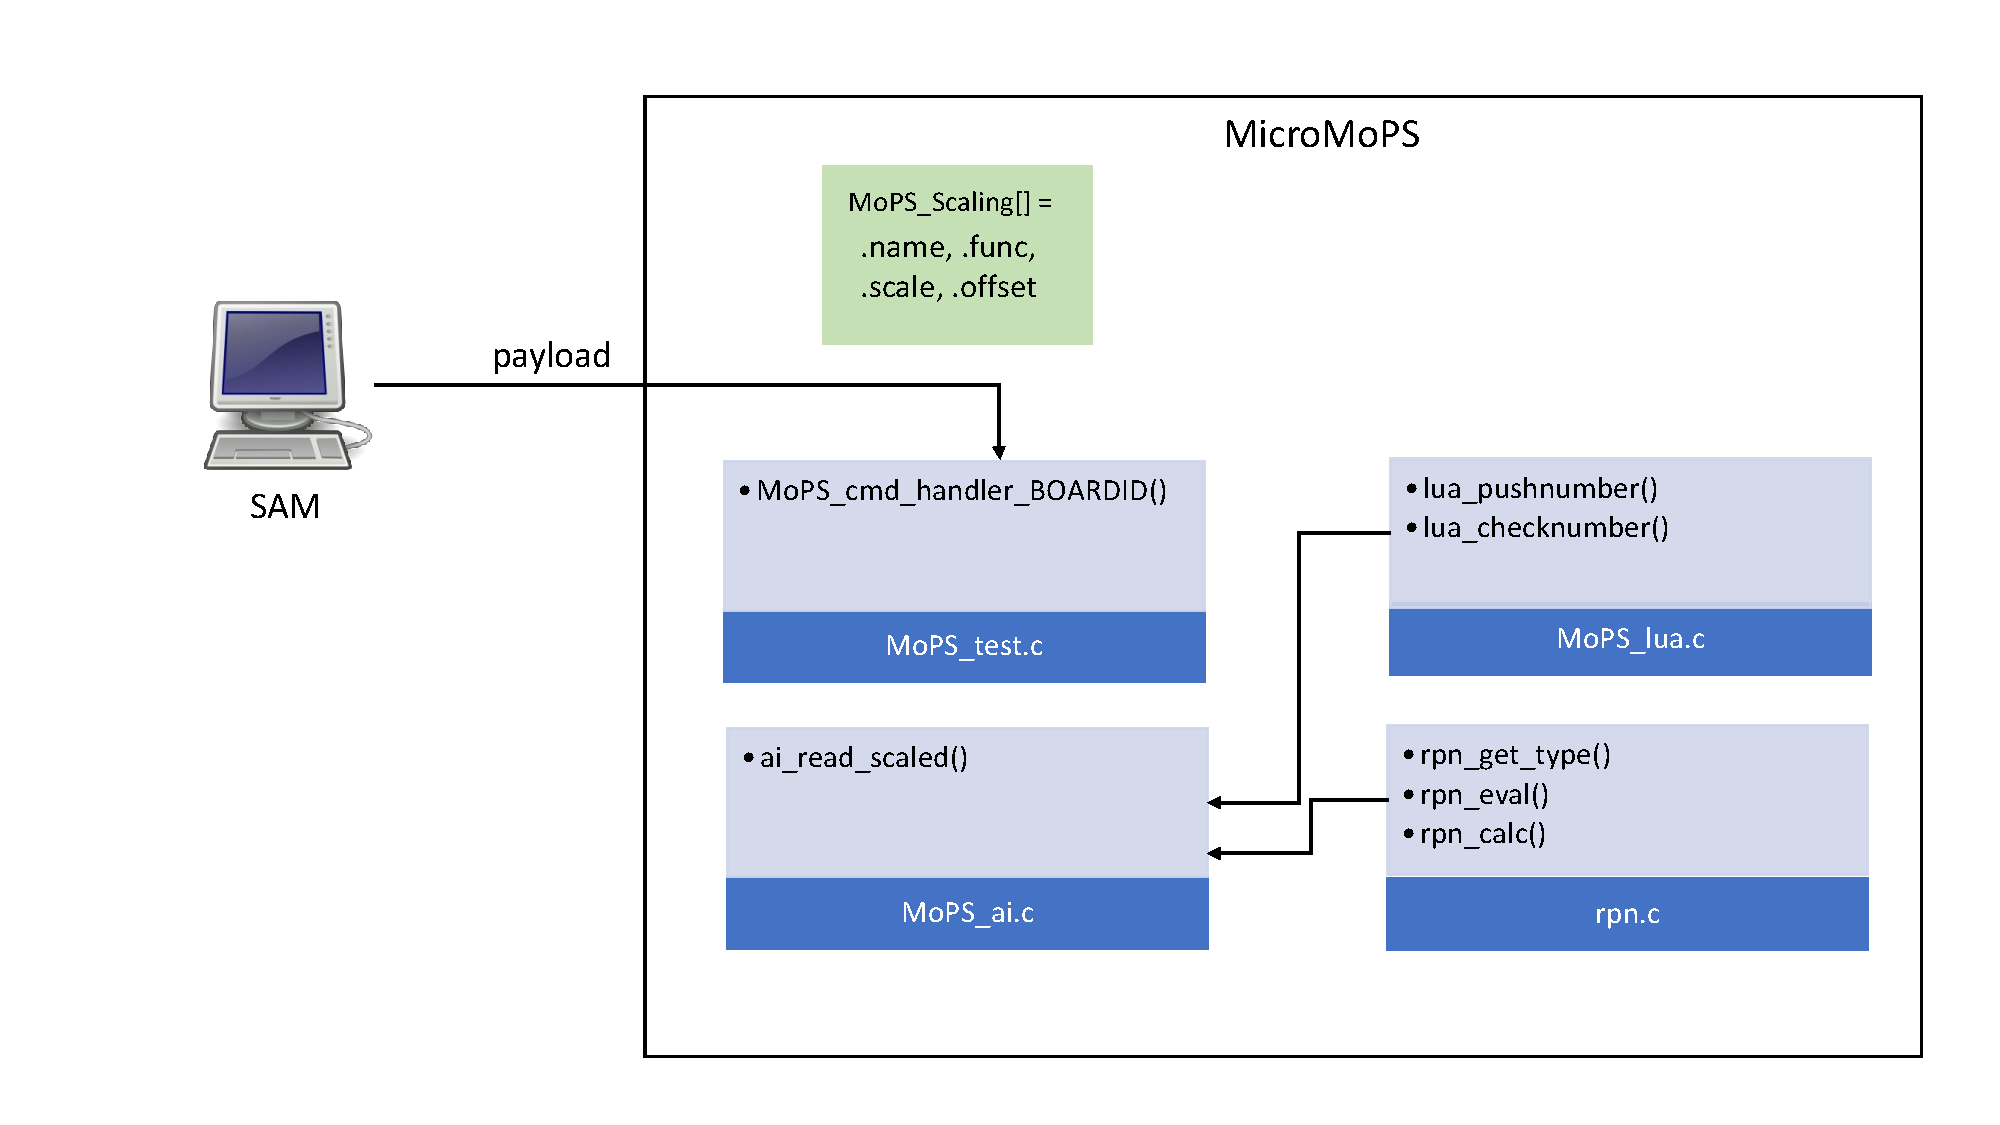
\includegraphics[trim=50 30 0 0, clip, width=152mm, scale=1]{images/Scaling_implementation.pdf}
		\caption{Implementation of data processing module}
		\label{fig:DP}
\end{figure}

\section{Compute scaling mechanisms in MicroMoPS}\label{sec:scaling}
	 In this work, linear scaling formula (see \cref{sec:linear function}) and Reverse Polish notation (see \cref{sec:RPN}) are implemented within the Lua handler of analog input module of MicroMoPS. 
	 The linear scaling formula uses the updated scaling parameters to process the analog measurements. 
	 RPN computation is achieved by making use of three fundamental handlers, such as `rpn\_get\_type()',
	 `rpn\_eval()' and `rpn\_calc()'. These handlers are defined in the `rpn.c' file (see \cref{fig:DP}). 
	 The `rpn\_get\_type()' handler is meant for decoding the respective operations or tokens based on the string data that is received from the SAM. The allowed operations in the RPN module are float variables, addition, subtraction, multiplication, division, square root, minimum function, and maximum function.
	 From the decoded type the respective operation is performed through the `rpn\_eval()' handler. The `rpn\_calc()' handler makes use of `rpn\_get\_type()' and `rpn\_eval()' handlers to perform the RPN computation. Along with the mentioned handlers the `rpn\_calc()' handler makes use of some of the functions that are part of Lua interpreter to memory efficiently (see \cref{sec:RPN}) perform the RPN computation. Finally, the MoPS\_scaling module (ai\_read\_scaled()) makes use of either `rpn\_calc()' or linear scaling formula to process the data using dynamically parsed scaling parameters (see \cref{sec:parse}).  
The operation of the RPN scaling mechanism is tested by hard coding the RPN string (see \cref{sec:RPN}) to channel-specific .func variable (updated in the config file).
Hard coding of RPN string is achieved by communicating the RPN string from TinyHost to MicroMoPS.
\afterpage{\null\newpage}
\afterpage{\null\newpage}
%\cleardoubleplainpage
%cleardoubleplainpage
\chapter{Evaluation and Analysis}
The enhancement in the existing software architecture to improve the processing speed of DUT electrical measurements are evaluated and analysed in this chapter. 
The processing capabilities of Reverse Polish Notation and linear scaling function are evaluated by measuring their time and memory consumption in performing the scaling computation. 
In order to compute Reverse Polish Notation or linear scaling function, a piece of code is written in the digital processing module of MicroMoPS. 
Scaling operation is performed as many times as the number of communication channels that are present in the MicroMoPS (see \cref{sec:parse}). The scaling operation comes as a part of the execution of test plans, and the Lua modules or classes that are specific to scaling are used in the test plan script to invoke the corresponding Lua C-API of MoPS-CORE microcontroller firmware. The Lua class that is meant for invoking the scaling function corresponding C-API i.e., `ai\_read\_scaled()' (see \cref{sec:scaling}) is `ai' ~\cite{Steinwender2016}. The real-time performance of the scaling operations is tested by invoking the scaling function multiple times from the TinyHost (see \cref{sec:TinyHost}), while the test plan is not running. Before invoking scaling functions setting some of the configurations (see \cref{fig:tinyhost}) that are specific to the communication channel is necessary. These test runs of a scaling operation are done at a very indeterministic interval to determine the stable values of the time that is consumed by the scaling operation. The time measurements that are recorded during the test runs are approximated to the closest simpler representation.        
The real-time performance of Reverse Polish Notation and linear scaling function is discussed in the following sections. 
%The calculation of time and memory consumption of the "Reverse polish notation" are as follows:

\section*{Real-Time performance of RPN function}

As described in the \cref{sec:scaling}, the `ai\_read\_scaled()' handler makes use of `rpn\_calc()` handler to perform RPN computation. The Memory consumption of the RPN is calculated by investigating the code that is associated in performing the RPN. The code snippet which performs the data processing (RPN) computation is built by using several local variables that are specific to `rpn\_calc()` (see \cref{fig:DP}) handler. The memory consumption of each of the local variables that are part of `rpn\_calc()' is as follows:  
\begin{enumerate}
\item rpn\_string = 32 bytes (max)
\item *temp(char) = 1 byte
\item *delim(char) = 1 byte
\item is valid(bool) = 1 byte
\item *save(char) = 1 byte
\item *snippet(char) = 1 byte
\item lua\_number -- res, a, b (float) = 4bytes*3 = 12 bytes
\end{enumerate}
The sum of the memory consumption of the local variables that are part of `rpn\_calc()' is \textbf{49 bytes}.
\\
\\
Consumption of time in performing RPN function is calculated by making use of the `time\_it()' handler from the `MoPS\_time.c' module. The calculation of the consumption of time is done for around 50 test runs. After around 50 test runs, the range of consumption of time to perform RPN is calculated. The time consumed by the RPN function approximately ranges from \textbf{\SIrange{45}{66}{\micro\second}}.

\section*{Real-Time performance of Linear scaling mechanism}

Similarly, the real-time performance of "Linear scaling mechanism" is measured by calculating the time and memory consumption of the code that performs the computation. 
The Memory consumption of the linear scaling mechanism is calculated by investigating the code that is associated in performing the linear scaling function.
Mere linear scaling equation is implemented within a `ai\_read\_scaled()' handler to perform the processing (linear scaling function) of data. 
The Memory consumption of each of the local variables that are part of linear scaling mechanism is as follows:

\begin{enumerate}
\item scale (float) = 4 bytes
\item digital\_result (float) = 4 bytes
\item offset (float) = 4 bytes 
\end{enumerate}                         
The sum of the memory consumption of the local variables that are part of linear scaling function is \textbf{12 bytes}.

The method of calculation of time consumption remains the same as how it is done for RPN function. Also, for the calculation of consumption of time to compute linear scaling function, around 50 samples of measurements are taken. The time consumed by linear scaling mechanism approximately ranges from \textbf{\SIrange{29}{134}{\nano\second}}.

\begin{figure}[hbt]
		\centering
		%\makebox[\textwidth]{%
		%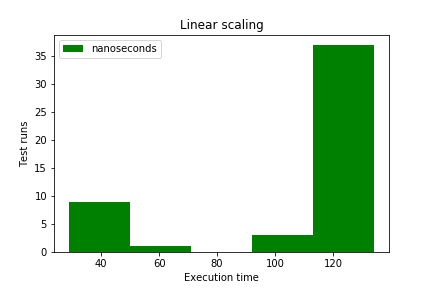
\includegraphics[trim=0 55 0 210, clip, width=210mm, scale=0.75]{images/linear_scaling.png}
		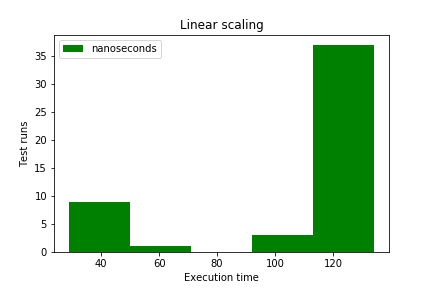
\includegraphics[width=0.6\textwidth]{images/linear_scaling.png}
		%\hfill
		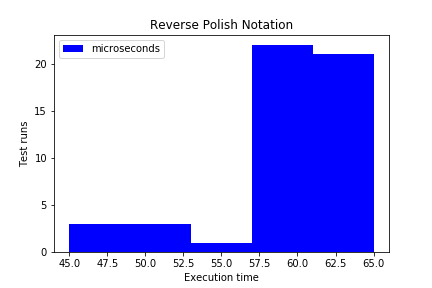
\includegraphics[width=0.6\textwidth]{images/rpn.png}
		\caption{Distribution of execution time of the scaling functions}
		\label{fig:Histogram}
\end{figure}

The distribution of the execution time of the linear scaling and Reverse Polish Notation function is as shown in the \cref{fig:Histogram}. The test runs of scaling computation are performed in this sophisticated stress test environment to record the time that is consumed by the scaling operation. At rare times the execution time of the scaling computation lies closer towards the \gls{BCET} of the given scaling computation because of the less interrupt load during the scaling operation. However, most of the other times the execution time of the scaling computation varies around the \gls{WCET} of the given scaling computation because of the substantial interrupt load during the scaling operation. In the case of a linear scaling mechanism, out of 50 disordered test runs, 8 to 10 test runs that records the execution time lies between 29 and 70 nanoseconds, and the rest of the test runs that records the execution time lies between 95 and 134 nanoseconds. Similarly, in the case of Reverse Polish Notation, out of 50 disordered test runs, 2 to 4 test runs that records the execution time lies between 45 and 57.5 microseconds, and the rest of the test runs that records the execution time lies between 57.5 and 65 microseconds. From the obtained execution time distribution, it can be inferred that there exists the stable region around the \acrshort{WCET}, which means almost all the times regardless of the increase or decrease of test runs from 50, the execution time of scaling operation only keeps moving within the stable region and at rare times towards the \acrshort{BCET}. 
The stable region for Reverse Polish Notation and linear scaling function lies between 95 and 134 nanoseconds, and 57.5 and 65 microseconds, respectively.            

The real-time performance comparison of Reverse Polish Notation and linear scaling mechanism is as shown in the Table 6.1.

\begin{table}[hpt]
	\centering
	\label{Table:scaling}
	\caption{Real-time performance comparision}
	\begin{tabular}{|p{4cm}||p{2.5cm}|p{2.7cm}||p{2.7cm}| } 
 	\hline
 	\textbf{Scaling mechanism}   &\textbf{Time}    &\textbf{Memory}    &\textbf{Test runs}\\
 							&\textbf{consumption}    &\textbf{consumption}  &\textbf{}\\
 	\hline
	RPN   &{45 $\mu$s - 66 $\mu$s}   &49 bytes &{$\approx$50}\\
 	\hline
	Linear scaling   &{29 ns - 134 ns}   &12 bytes &{$\approx$50}\\
 	\hline
	\end{tabular}
\end{table}

%\begin{figure}[hbt]
%		\centering
	%	%\makebox[\textwidth]{%
		%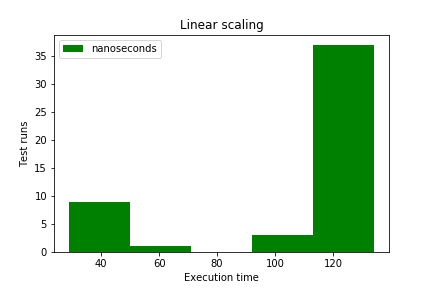
\includegraphics[trim=0 55 0 210, clip, width=210mm, scale=0.75]{images/linear_scaling.png}
		%\begin{minipage}[b]{0.9\textwidth}
		%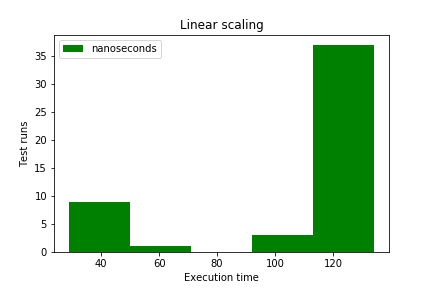
\includegraphics[width=0.4\textwidth]{images/linear_scaling.png}
		%\hfill
		%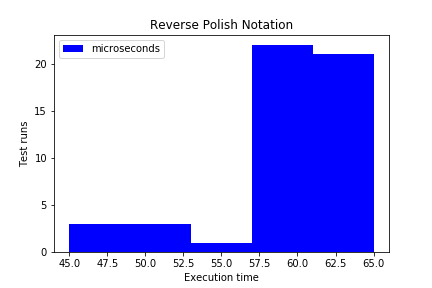
\includegraphics[width=0.5\textwidth]{images/rpn.png}
		%\caption{Distribution}
		%\label{fig:Histogram}
		%\end{minipage}
		%\hfill
		%\begin{minipage}[b]{0.9\textwidth}
		%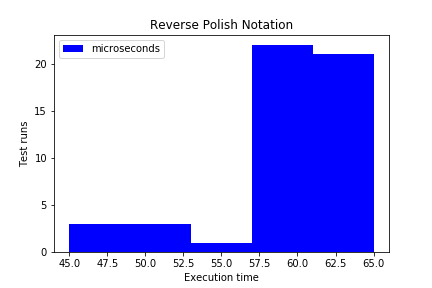
\includegraphics[width=0.4\textwidth]{images/rpn.png}
		%\hfill
		%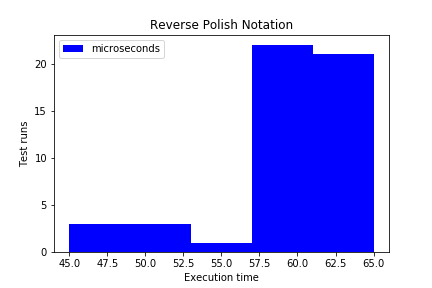
\includegraphics[width=0.5\textwidth]{images/rpn.png}
		%\caption{Distribution}
		%\label{fig:Histogram2}
		%\end{minipage}
%\end{figure}


%\begin{figure}[hbt]
	%	\centering
		%\makebox[\textwidth]{%
		%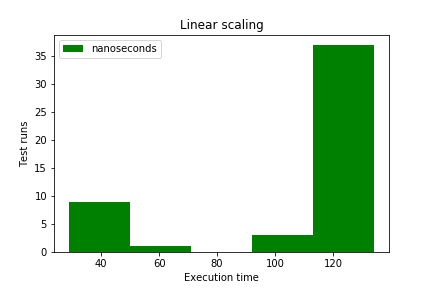
\includegraphics[trim=0 55 0 210, clip, width=210mm, scale=0.75]{images/linear_scaling.png}
		%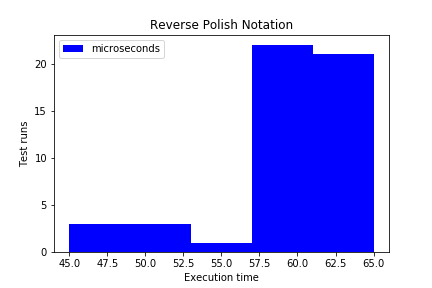
\includegraphics[width=0.5\textwidth]{images/rpn.png}
		%%\hfill
		%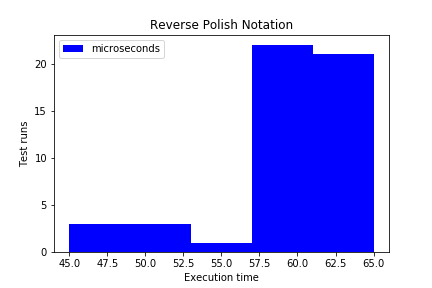
\includegraphics[width=0.5\textwidth]{images/rpn.png}
		%\caption{Distribution of execution time of the scaling functions}
		%\label{fig:Histogram2}
%\end{figure}

From Table 6.1, it can be concluded that the linear scaling mechanism consumes less time and memory in comparison with the Reverse Polish Notation function. 
This, further implies that the linear scaling mechanism is more real-time efficient scaling mechanism compared to Reverse Polish Notation. 

On the other hand, the entire procedure of resolution of board UIDs from multiple different sources such as the test plan, board and scaling database in web server, board UIDs communication from MicroMoPS, and subsequent communication of scaling parameters to the data processing system of MicroMoPS supports to an automation of processing of analog measurements in the stress test environment regardless of any plausible combination of hardware target, application module and DUT.
Every plausible combination of boards correspond to an individual type of stress test application. The main benefit of the automation of the processing of data is the avoidance in the maintenance of the scaling database of every application-specific stress test system in the control module. This results in a conservation of quite an amount of memory of the MicroMoPS. Also, by automating the processing of data, the method of manual feed of scaling values is avoided, which helps in minimizing human error.  
%As a result, the scaling operation is automatically performed irrespective of the stress test applications that are performed. 

\section{Answers to the Research questions}
The above analysis and evaluation of the results bring a conclusion to the raised research questions (see \cref{sec:RQs}).

\begin{itemize}
	\item By analysis of the various existing application boards, a linear model solution could be found.
		The performance of the linear model over the Reverse Polish Notation model is greatly enhanced. 
	\item The derivation of a linear scaling mechanism and their precise conversion of analog measurements into control module-specific voltages, proves the possibility of a linear scaling mechanism in this stress test environment. 
	\item The resolution of board UIDs and the filtering of scaling values establishes the automation of data processing.
		This exhibits the possibility of automated processing of analog measurements in this stress test environment.  
\end{itemize}
%\begin{tabular}{ |p{3cm}|p{5cm}|p{2cm}| }
 %\hline
 %\multicolumn{3}{|c|}{Real-time performance comparision } \\
 %\hline
 %\textbf{Scaling mechanism}   & \textbf{Time consumption}    &\textbf{Memory consumption} \\
%RPN   &45 us - &66 us   &49 bytes \\
%Linear scaling   &29 ns - 134ns   &12 bytes \\
 %\hline
%\end{tabular}
%\label{Table5}

\afterpage{\null\newpage}
\afterpage{\null\newpage}
\afterpage{\null\newpage}
%\cleardoubleplainpage
\chapter{Summary and Outlook}

\section{Summary}

In this sophisticated stress test environment to improve the data processing mechanism, the electrical circuits that are associated with measuring the physical quantities that generate in a semiconductor, are analyzed.
A classical linear scaling mechanism is introduced to the data processing system of a control module by analyzing the measurement circuits.
Also, the Reverse Polish Notation scaling computation function is incorporated into the data processing system of the control module which opens up the possibility of performing a complex level of scaling functions.

The boards that are present in the stress test environment are identified by the extraction of the respective board ids.
The extraction of board ids and their correspondence in the resolution of board information coming from different sources such as test plan and MoPS web server, led to the automation of processing of analog measurements that generate in the semiconductor, irrespective of the stress test application. 

The automation in the processing of analog measurements has simplified the writing procedure of test plans and manual scaling is no more involved within the test plans. 
Human error is minimized because of the automated method of scaling.   
The improved data processing mechanism is implemented and tested in the KAI lab. 

\section{Outlook}

Real-time efficient scaling mechanism and automation of processing of analog measurements provide gateway for conducting advanced application stress testing in the stress test environment.
The newly introduced scaling mechanism known as Reverse Polish Notation can be used for further improvement of a scaling function. The gain function introduced by a 
differential operational amplifier itself could be a non-linear function. The differential input/output impedance of an operational amplifier can be of a significant effect 
in calculation of discrete voltage values specfic to control module. The internal circuits of the differential operational amplifier can be analysed and the
contribution from its gain function in performing the scaling can be described using Reverse Polish Notation. The implementation of the Lua interpreter influences in the real-time performance of the Reverse Polish Notation because the RPN uses Lua stack to perform the scaling operation. Lua interpreter even though it utilizes a minimum of RAM because of its implementation in Lua, there is a scope to optimize the implementation of the Lua interpreter. Optimization of the implementation of the Lua interpreter results in the improved execution time performance of the Reverse Polish Notation. Similarly, the execution time performance of Reverse Polish Notation could significantly be improved by replacing the division operation that takes place during the scaling computation by right shifting 12 times the digital output along with some operation to handle the decimal result. 

%\include{Outlook.tex}
%	Bibliography, Acronyms, Symbols ...
\afterpage{\null\newpage}
\afterpage{\null\newpage}
\printbibliography
%\glsaddall
%\cleardoubleplainpage
\afterpage{\null\newpage}
\printnoidxglossaries
%\printglossary
\end{document}
